% !TEX options=--shell-escape
% Thesis template by Julian Lueken

% Optimized for literature management with JabRef + BibLaTeX

% Change user settings:
%	"keep_focus": true, --> false, to remove the annoying pop ups
%	"use_biblatex": false,
%	"builder": "traditional" --> "basic", to use biber on every compilation
\documentclass[a4paper, 11pt]{report}

% Packages
%% Input encoding
\usepackage[T1]{fontenc}
\usepackage{lmodern}
%%\usepackage[utf8]{inputenc}

%% Syntax
\usepackage{ifthen}

%% Languages and symbols
\usepackage[main=english]{babel}
\usepackage{extarrows}
\usepackage{marvosym}

%% AMS packages
\usepackage{amssymb}
\usepackage{amsmath}
\usepackage{amsthm}

%% Citations and references
\usepackage[style=alphabetic, backend=biber]{biblatex} 
\usepackage[hidelinks]{hyperref}
\usepackage{csquotes}
\usepackage{nameref}
\usepackage{cleveref}
\usepackage{listings}

%% Page geometry
\usepackage[onehalfspacing]{setspace}
\usepackage[top=30mm, left=25mm, right=25mm, bottom=20mm]{geometry}
\usepackage{titlesec}

%% Figures and graphics
\usepackage{graphicx}
\usepackage{xcolor}
\usepackage{colortbl}
\usepackage{subcaption}
\usepackage{tikz}
\usepackage{float}
\usepackage{svg}

%% Pseudo-code
\usepackage{algorithm}
\usepackage[noend]{algpseudocode}

%% Testing
\usepackage{lipsum}

%% Package settings
%%% BibLaTeX resource (JabRef output file)
\addbibresource{../bibtex/bibliography.bib}

%%% Hyperref options
\hypersetup{hypertexnames=false}

%%% Listings options (for writing code in LaTeX)
\lstset{numbers=left, numberstyle=\tiny, numbersep=5pt}
\lstset{language=Python}

%%% AMS environment definitions
\theoremstyle{definition}
\newtheorem{definition}{Definition}[section]
\newtheorem{example}[definition]{Example}
\newtheorem{theorem}[definition]{Theorem}
\newtheorem{corollary}[definition]{Corollary}
\newtheorem*{remark}{Remark}
\newenvironment{myAbstract}{\section*{Abstract}}{}

%%% Special formatting
\renewcommand{\emph}[1]{\textit{#1}}
\newcommand{\mytitle}[1]{\LARGE{#1}\normalsize\\[0.3em]}
\newcommand{\titlespace}{\vspace{2em}}
\newcommand{\smallspace}{\vspace{1em}}
\newcommand{\hugespace}{\vspace{17em}}
\newcommand{\logoheight}{4em}
\newcommand{\derivative}[2]{\frac{\textrm{d}{#1}}{\textrm{d}{#2}}}
\newcommand{\domrestr}{\big|}

\DeclareMathOperator{\arctantwo}{arctan2}

%% Special formatting for pesudocode
\algblock{Input}{EndInput}
\algnotext{EndInput}
\algblock{Output}{EndOutput}
\algnotext{EndOutput}
\newcommand{\Desc}[2]{\State \makebox[12em][l]{#1}#2}


\begin{document}

% Chapter format
\titleformat{\chapter}[hang]{\normalfont\huge\bfseries}{\thechapter}{0.75em}{\huge\bfseries}
\titlespacing*{\chapter}{0em}{0em}{1em}

% Title page
\pagenumbering{gobble}
\newgeometry{top=35mm, left=20mm, right=20mm, bottom=10mm}
\begin{titlepage}
	\begin{center}
		\begin{minipage}{.49\textwidth}
			\flushleft
			
\includegraphics[height=\logoheight]{../assets/formal/logo_gau.png}
		\end{minipage}
		\begin{minipage}{.49\textwidth}
			\flushright
			
\includegraphics[height=\logoheight]{../assets/formal/logo_dlr.png}	
		\end{minipage}
		\begin{minipage}{.49\textwidth}

			\begin{center}
				\vspace{2cm}
				Master's thesis in\\
				Applied Computer Science\\
				\titlespace
				\mytitle{CoolingGen}
				A parametric 3D-modeling software for turbine blade cooling geometries using NURBS\\
				\titlespace
				\today\\
				\hugespace
				Institute for Numerical and Applied Mathematics at the Georg-August-University Göttingen\\
				\titlespace
				Institute for Propulsion Technology at the German Aerospace Center in Göttingen\\
				\titlespace
				Bachelor's and master's theses at the Center for Computational Sciences at the Georg-August-University Göttingen\\
				\titlespace
				Julian Lüken\\
				\texttt{julian.lueken@dlr.de}\\
			\end{center}
		\end{minipage}
	\end{center}
\end{titlepage}
\pagebreak

% Address page
\pagestyle{empty}
\restoregeometry
\newgeometry{top=210mm, left=45mm, right=45mm}
\noindent
\begin{tabular}{l}
Georg-August-University Göttingen\\
Institute of Computer Science\\
\end{tabular}\\[1em]
\begin{tabular}{ll}
	\Telefon 	&+49 (551) 39-172000\\
	\FAX 		&+49 (551) 39-14403\\
	\Letter 	&\texttt{office@cs.uni-goettingen.de}\\
\end{tabular}\\[1em]
\begin{tabular}{l}
\texttt{www.informatik.uni-goettingen.de}\\
\end{tabular}\\[1em]
\pagebreak

% Done-it-myself page
\noindent I hereby declare that this thesis has been written by myself and no other resources than those mentioned have been used.\\[0.7em]
\phantom{H}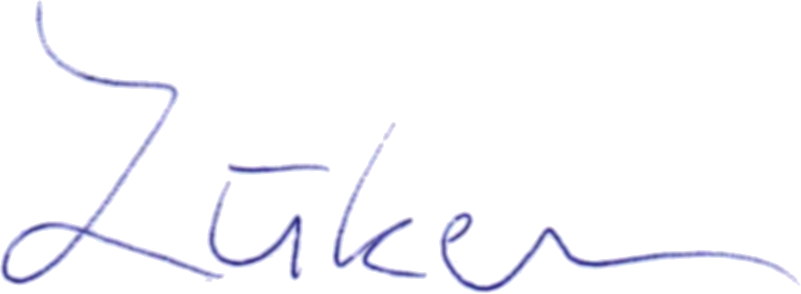
\includegraphics[height=3em]{../assets/formal/sign.png}\\[0.5em]
Göttingen, \today \hspace{2em}
\pagebreak

% Abstract and Zusammenfassung
\restoregeometry
\begin{abstract}
	\thispagestyle{plain}
	\pagenumbering{roman}
	\setcounter{page}{3}
	\lipsum[1-3]
\end{abstract}
\renewcommand{\abstractname}{Zusammenfassung}
\begin{abstract}
	\thispagestyle{plain}
	\pagenumbering{roman}
	\setcounter{page}{4}
	\lipsum[4-6]
\end{abstract}
\pagebreak

% Table of contents
\setcounter{page}{5}
\restoregeometry
\tableofcontents
\pagebreak

% Actual document starts here
\restoregeometry
\pagenumbering{arabic}
\setcounter{page}{1}
\pagestyle{plain}

\chapter{Introduction}
\section{Motivation}
\section{State of the Art}
\section{Problem Statement}

\chapter{Geometric Methods}\label{chap:methods}
	As stated before, Non-Uniform Rational B-splines (NURBS) curves and surfaces are used to model geometries in CoolingGen. In this chapter we will first introduce Bézier curves. We will then generalize Bézier curves to obtain B-spline curves and surfaces. Applying an embedding map and a projection map to B-spline curves and surfaces, we acquire NURBS curves and surfaces, which are a generalization of B-spline curves and surfaces. Furthermore, CoolingGen uses special geometric algorithms such as point projection, ray marching, curve intersection, offset curve creation and fillet creation, which we will also present.

\section{Bézier Curves}
	Bézier curves are named after the French engineer Pierre Bézier, who famously utilized them in the 1960s to design car bodies for the automobile manufacturer Renault \cite{Bezier1968}. Today, they are used in a wide variety of vector graphics applications (i.e. in font representation on computers). At first glance, the definition of the Bézier curve might seem cumbersome, but given the mathematical foundation and a few graphical representations, it becomes apparent why they are such a powerful tool in computer-aided design.

	\begin{figure}[H]
		\centering
		\begin{subfigure}{0.25\textwidth}
			\includesvg[width=\textwidth]{../python/bezierDifferentDegrees1}
			\caption{Degree $1$.}
		\end{subfigure}
		\begin{subfigure}{0.25\textwidth}
			\includesvg[width=\textwidth]{../python/bezierDifferentDegrees2}
			\caption{Degree $2$.}
		\end{subfigure}
		\begin{subfigure}{0.25\textwidth}
			\includesvg[width=\textwidth]{../python/bezierDifferentDegrees3}
			\caption{Degree $3$.}
		\end{subfigure}
		\caption{Bézier curves of different degrees (orange) and their control points (blue).}
		\label{fig:bezierdifferentdegrees}
	\end{figure}

\subsection{Definition}
	\begin{definition}
		The \emph{Bernstein basis polynomials} of degree $n$ on the interval $[t_0,t_1]$ are defined as
		\begin{equation}\label{eq:bernsteinbasisdef}
			b_{n,k,[t_0, t_1]}(t) := \frac{\binom{n}{k} (t_1-t)^{n-k}(t-t_0)^k}{(t_1-t_0)^n},
		\end{equation}
		for $k \in \{0,\dots, n\}$.
	\end{definition}

	\begin{definition}
		A \emph{Bézier curve} of degree $n$ is a parametric curve $B_{P,[t_0, t_1]}: [t_0, t_1] \rightarrow \mathbb{R}^d$ that has a representation
		\begin{equation}\label{eq:bezierdef}
			B_{P, [t_0, t_1]}(t) = \sum_{k=0}^n b_{n,k,[t_0, t_1]}(t) P_k = \sum_{k=0}^n \frac{\binom{n}{k} (t_1-t)^{n-k}(t-t_0)^k}{(t_1-t_0)^n} P_k.
		\end{equation}
		We call the elements of the set $P = \{P_0, P_1, \dots, P_n\} \subset \mathbb{R}^d$ the \emph{control points} of $B_P$.
	\end{definition}

	\begin{remark}
		Let $t_0 = 0$ and $t_1 = 1$. Then Equation (\ref{eq:bezierdef}) simplifies to
		\begin{equation*}
			b_{n,k}(t) := b_{n,k,[0,1]}(t) = \binom{n}{k} (1-t)^{n-k}t^k
		\end{equation*}
		and Equation (\ref{eq:bernsteinbasisdef}) simplifies to
		\begin{equation}\label{eq:bezierdefshort}
			B_P(t) := B_{P,[0,1]}(t)= \sum_{k=0}^n \binom{n}{k} (1-t)^{n-k}t^k P_k.
		\end{equation}
		This case is the only case considered in this thesis.
	\end{remark}

	In a Bézier curve of a given degree, the control points completely determine the shape of the curve. This behavior can be observed in Figure \ref{fig:bezierdifferentdegrees}. However, changing one control point affects the whole curve, since for $n$ control points the degree of the Bézier curve is always $n-1$. This behavior also becomes apparent using de Casteljau's algorithm for the computation of points on the Bézier curve.

\subsection{De Casteljau's Algorithm}
	The computation of Equation (\ref{eq:bezierdefshort}) is usually performed using de Casteljau's algorithm. This is because the algorithm yields a simple implementation and lower complexity than straightforwardly computing Equation (\ref{eq:bezierdefshort}). The algorithm was proposed by Paul de Faget de Casteljau for the automobile manufacturer Citroën in the 1960s.

	\begin{algorithm}[H]
		\begin{algorithmic}[1]
			\Input
				\Desc{$P = \{P_0, P_1, ..., P_n\}$}{set of control points}
				\Desc{$t$}{real number}
			\EndInput
			\Output
				\Desc{$P^{(n)}_0 = B_P(t)$}{the point on the Bézier curve w.r.t. to $t$}
			\EndOutput

			\caption{de Casteljau's algorithm}\label{alg:decasteljaualgo}
			\Procedure{deCasteljau}{$P, t$}
				\State $P^{(0)} \gets P$
				\For {$j = 1, 2, ..., n$}
					\For {$k = 0, 1, ..., n-j$}
						\State $P^{(j)}_k \gets (1-t) \cdot P^{(j-1)}_k + t \cdot P^{(j-1)}_{k+1}$
					\EndFor
				\EndFor
				\State \Return $P^{(n)}_0$
			\EndProcedure
		\end{algorithmic}
	\end{algorithm}

	\begin{theorem}
		Algorithm \ref{alg:decasteljaualgo} computes $B_P(t)$.
	\end{theorem}
	\begin{proof}
		By induction. Let $n = 1$ and $t \in [0,1]$ be fixed. Then
			$$ P_0^{(1)} = (1-t) \cdot P_0 + t \cdot P_1.$$
		By employing the induction hypothesis
			$$ P_j^{(n)} = \sum_{k=j}^{n+j} \binom{n}{k} (1-t)^{n-k}t^k P_{j+k}$$
		for some $n \in \mathbb{N}$, we can infer that
		\begin{align*}
			P_0^{(n+1)}	&= (1-t) \cdot P_0^{(n)} + t \cdot P_1^{(n)} \\
						&= (1-t) \cdot \sum_{k=0}^{n} \binom{n}{k} (1-t)^{n-k}t^k P_{k} + t \cdot \sum_{k=1}^{n+1} \binom{n}{k} (1-t)^{n-k}t^k P_{k+1} \\
						&= \sum_{k=0}^{n+1} \binom{n+1}{k} (1-t)^{n+1-k}t^k P_{k},
		\end{align*}
		which is equal to $B_P(t)$ for degree $n+1$.
	\end{proof}

	A visual representation of Algorithm \ref{alg:decasteljaualgo} yields a triangular scheme. To compute one point on a Bézier curve $B_P$ with degree $n$, one has to perform $\frac{n^2-n}{2}$ vector additions and $n^2-n$ scalar multiplications.

	\begin{figure}[H]
		\centering
		\begin{subfigure}{0.49\textwidth}
			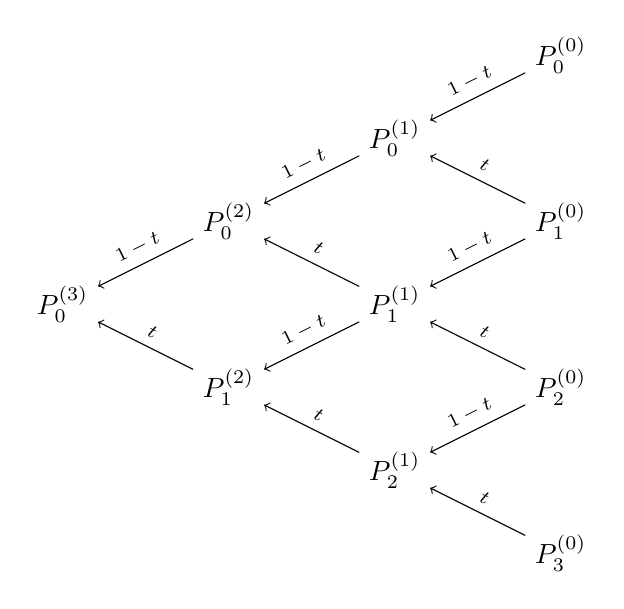
\begin{tikzpicture}
				\def\dx{60pt}
				\def\dy{30pt}

				\pgfmathsetmacro{\degree}{3}

				% Make nodes
				\newcounter{i}
				\newcounter{j}

				\node (\arabic{i}) at (0,0) {$P^{(\degree)}_0$};
				\stepcounter{i}

				\foreach \x in {1, ..., \degree} {
					\pgfmathsetmacro{\xstep}{\x-2}

					\setcounter{j}{0}
					\foreach \y in {\x, \xstep, ..., -\x} {
						\node (\arabic{i}) at (\x*\dx, \y*\dy) {$P^{(\pgfmathint{\degree-\x}\pgfmathresult)}_{\arabic{j}}$};
						\stepcounter{i}
						\stepcounter{j}
					}
				}
				
				% Make arrows
				\newcounter{z}
				\newcounter{a}
				\newcounter{b}
				\pgfmathsetmacro{\maxx}{\degree}
				\foreach \x in {1,...,\degree}{
					\foreach \y in {1,...,\x}{
						
						\setcounter{a}{\arabic{z}}
						\addtocounter{a}{\x}

						\setcounter{b}{\arabic{z}}
						\addtocounter{b}{\x}
						\stepcounter{b}
						
						\draw [<-] (\arabic{z}) -- (\arabic{a}) node[above, midway, sloped] {\scriptsize $1-t$};
						\draw [<-] (\arabic{z}) -- (\arabic{b}) node[above, midway, sloped] {\scriptsize $t$};
						
						\stepcounter{z}
					}
				}
			\end{tikzpicture}
			\caption{Algorithmic visualization.}
		\end{subfigure}
		\hfill
		\begin{subfigure}{0.49\textwidth}
			\includesvg[width=\textwidth]{../python/deCasteljauVisual}
			\caption{Geometric visualization of $B_P(\frac{3}{5})$.}
		\end{subfigure}
		\caption{Visual representations of de Casteljau's algorithm.}
		\label{fig:decasteljautriangle}
	\end{figure}

	Interestingly, the representation of the algorithm in Figure \ref{fig:decasteljautriangle} also gives rise to an intuitive visualization of the geometric shape of the Bézier curve $B_P$. For all $i \in \{0, ..., n\}$ and all $j \in \{0, ..., n-i\}$, the point $P^{(i+1)}_j$ is the convex combination (always w.r.t. $t$) of $P^{(i)}_j$ and $P^{(i)}_{j+1}$. Thus $P^{(i+1)}_j$ always lies on the line segment between $P^{(i)}_j$ and $P^{(i)}_{j+1}$, as can be observed in the example in Figure \ref{fig:decasteljautriangle}.

\subsection{Properties}
	Other than being remarkably intuitive, Bézier curves have a lot of covenient properties. In computer-aided design software, most graphical user interfaces rely on the principle of letting the user interactively drag and drop the control points with a mouse, granting them control over the shape of the whole Bézier curve. The following theorems further illustrate why this is a good concept.

	\begin{theorem}\label{thm:bezierendpoints}
		We have $B_P(0) = P_0$ and $B_P(1) = P_n$.
	\end{theorem}
	\begin{proof}
		Explicit computation for $t=0$ and $t=1$ yields
			$$B_P(0) = \sum_{k=0}^n \binom{n}{k} t^k P_k = \binom{n}{0} P_0 = P_0$$
		and
			$$B_P(1) = \sum_{k=0}^n \binom{n}{k} (1-t)^{n-k} P_k = \binom{n}{n} P_n = P_n.$$
	\end{proof}

	\begin{theorem}\label{thm:bezieraffinetransform}
		Let $T \in \mathbb{R}^{3 \times 3}$. Then $B_{TP}(t) = TB_P(t)$ where $TP := \{TP_0, TP_1, ..., TP_n\}$.
	\end{theorem}
	\begin{proof}
		For all $t \in [0, 1]$ we can directly compute
			$$TB_P(t) = \sum_{k=0}^n \binom{n}{k} (1-t)^{n-k}t^k TP_k = B_{TP}(t).$$
		This property is called invariance with respect to linear transforms.
	\end{proof}

	\begin{theorem}\label{thm:bezierconvexhull}
		The Bézier curve $B_P(t)$ lies in the convex hull of $P$ for all $t \in [0,1]$.
	\end{theorem}
	\begin{proof}
		By the algorithm of de Casteljau (\ref{alg:decasteljaualgo}), we know that $P^{(i)}_j = (1-t) \cdot P^{(i-1)}_j + t \cdot P^{(i-1)}_{j+1}$ for all $t \in [0, 1]$. Therefore, $P^{(i)}$ lie in the convex hull of $P^{(i-1)}$. But then $B_P(t) = P^{(n)}_0$ always lies in the convex hull of $P^{(0)} = P$ by induction.
	\end{proof}

	Theorem \ref{thm:bezierendpoints} guarantees the control over the end points of the the curve, whereas Theorem \ref{thm:bezierconvexhull} ensures that the Bézier curve lies close to the control points. Theorem \ref{thm:bezieraffinetransform} shows that transformations such as rotations and projections can be applied directly to the control points instead of the points on the curve.

	Simple as their appearance may be, Bézier curves fall short of representing some of the most common geometric shapes. Given a finite number of control points, we can never make $B_P(t)$ a circular arc, although a circle has a very simple parametric form. One of their greatest perks, the ability to describe a shape with a low number of of control points, is simultaneously one of their greatest shortcoming. This is most likely the reason why Bézier curves are not the state of the art in technical engineering applications. However, Bézier curves certainly do provide an intuition for Non-Uniform Rational B-Splines or NURBS, which is their prevailing counterpart.

\section{Non-Uniform Rational B-splines (NURBS)}
	NURBS are a state of the art tool for curve and surface modelling. There is a somewhat common joke that describes the acronym NURBS as \emph{"Nobody Understands Rational B-Splines"} (source?). In this section, we invalidate this punch line. First of all, we discuss B-splines, then we construct B-spline curves and surfaces and then we apply simple transformations to the B-spline curves and surfaces to acquire NURBS curves and surfaces.

\subsection{Definition}
	Similarly to how Bézier curves are defined on the Bernstein polynomial basis, NURBS are defined on basis functions called basis splines or, more commonly, B-splines.

	\begin{definition}
		A \emph{knot sequence} $(t_m)_{m=-\infty}^{\infty} \subset \mathbb{R}$ is a sequence with $t_{m} \leq t_{m+1}$ for all $m \in \mathbb{Z}$.
	\end{definition}

	\begin{definition}
		The \emph{B-splines of degree $0$} on a knot sequence $(t_m)$ are defined as
		\begin{equation}
			N^{(t_m)}_{1,k}(t) :=
			\begin{cases}
				1 & \text{if } t \in [t_k, t_{k+1}),\\
				0 & \text{else.}
			\end{cases}
		\end{equation}
		The \emph{B-splines of degree $p-1$} with $p > 1$ are given by the \emph{Cox-de-Boor recursion formula}
		\begin{equation}\label{eq:coxdeboorrec}
			N_{p,k}^{(t_m)}(t) := \omega^{(t_m)}_{p-1, k}(t) \, N^{(t_m)}_{p-1, k}(t) + (1-\omega^{(t_m)}_{p-1, k+1}(t)) \, N^{(t_m)}_{p-1, k+1}(t),
		\end{equation}
		where
		\begin{equation}
			\omega^{(t_m)}_{p,k}(t) := 
			\begin{cases}
				\frac{t-t_k}{t_{k+p} - t_k} &\text{if } t_{k+p} \neq t,\\
				0 							&\text{else.}
			\end{cases}
		\end{equation}
	\end{definition}

	\begin{remark}
		Instead of $N_{p,k}^{(t_m)}$ we write $N_{p,k}$ and explicitly refer to $(t_m)$ when necessary. We restrict the domain of definition of $N_{p,k}$ to $[0, 1]$ by setting $\lim_{m \to -\infty} t_m = 0$ and $\lim_{m \to \infty} t_m = 1$.
	\end{remark}

	\begin{definition}
		A \emph{B-spline curve} of degree $p-1$ over a set of control points
			$$P = \{P_0, P_1, ... P_n\} \subset \mathbb{R}^d$$
		and a knot sequence $(t_m)$ is defined as
			$$ S_P(t) = \sum_{k=0}^{n} N_{p,k}(t) P_k.$$
	\end{definition}

	\begin{definition}\label{def:nurbs}
		A \emph{NURBS curve} $C_P(t)$ of degree $p-1$ with the control points 
			$$P = \{P_0, P_1, ..., P_n\} \subset \mathbb{R}^d,$$ 
		the control weights $w = (w_0, w_1, ... w_n) \subset \mathbb{R}$ and a knot sequence $(t_m)$ is defined as
		\begin{equation}
			C_P(t) = \frac{\sum_{k=0}^n N_{p,k}(t) w_k P_k}{\sum_{k=0}^n N_{p,k}(t) w_k}.
		\end{equation}
	\end{definition}

	\begin{remark}
		Let $P \subset \mathbb{R}^d$. A NURBS curve can alternatively be understood as a projection of a B-spline curve on a transformed set of control points. For this purpose we define the embedding into the weighted vector space
			$$\Phi_w: \mathbb{R}^d \rightarrow \mathbb{R}^{d+1}$$
		that maps each control point $P_k = (p_1, ..., p_d) \in \mathbb{R}^d$ onto $(w_k p_1, ..., w_k p_d, w_k) \in \mathbb{R}^{d+1}$.
		We also have to define the projection map
			$$\Phi^\dagger: \mathbb{R}^{d+1} \rightarrow \mathbb{R}^d$$ 
		that maps each point on the B-spline curve $S_{\Phi(P)}(t) = (s_1, ..., s_d, s_{d+1})$ onto $(\frac{s_1}{s_{d+1}}, ..., \frac{s_d}{s_{d+1}})$.
		We can then define the NURBS curve as
				$$ C_P(t) = \Phi^\dagger(S_{\Phi_w(P)}(t)).$$ 
	\end{remark}

	Utilizing the notation with the embedding map $\Phi_w$ and the projection map $\Phi^\dagger$, we will calculate points on an arbitrary NURBS curve by calculating points on a corresponding B-spline curve. To do this, we employ the following steps on a set of control points $P$ and the weights $w$:
	\begin{enumerate}
		\item Calculate $P_w = \Phi_w(P)$.
		\item Calculate points on $S_{P_w}$.
		\item Project points onto $\mathbb{R}^d$ by applying $\Phi^\dagger$ to $S_{P_w}$ to find $C_P$.
	\end{enumerate}
	The calculation of points on a B-spline curve can be done similarly to the calculation of a point on a Bézier curve. The exact method is presented in the next section.

	\begin{theorem}
		Let $w \equiv 1$. Then $S_P \equiv \Phi^\dagger(S_{\Phi_w(P)})$. In other words, NURBS curves are a generalization of B-spline curves.
	\end{theorem}
	\begin{proof}
		Since in this case $\Phi_w((p_1, ..., p_d)) = (p_1, ..., p_d, 1)$, we have
			$$\Phi^\dagger(S_{\Phi_w(P)}(t)) = \Phi^\dagger(\Phi_w(S_P(t))) = S_P(t).$$
	\end{proof}

	\begin{figure}[H]
		\centering
		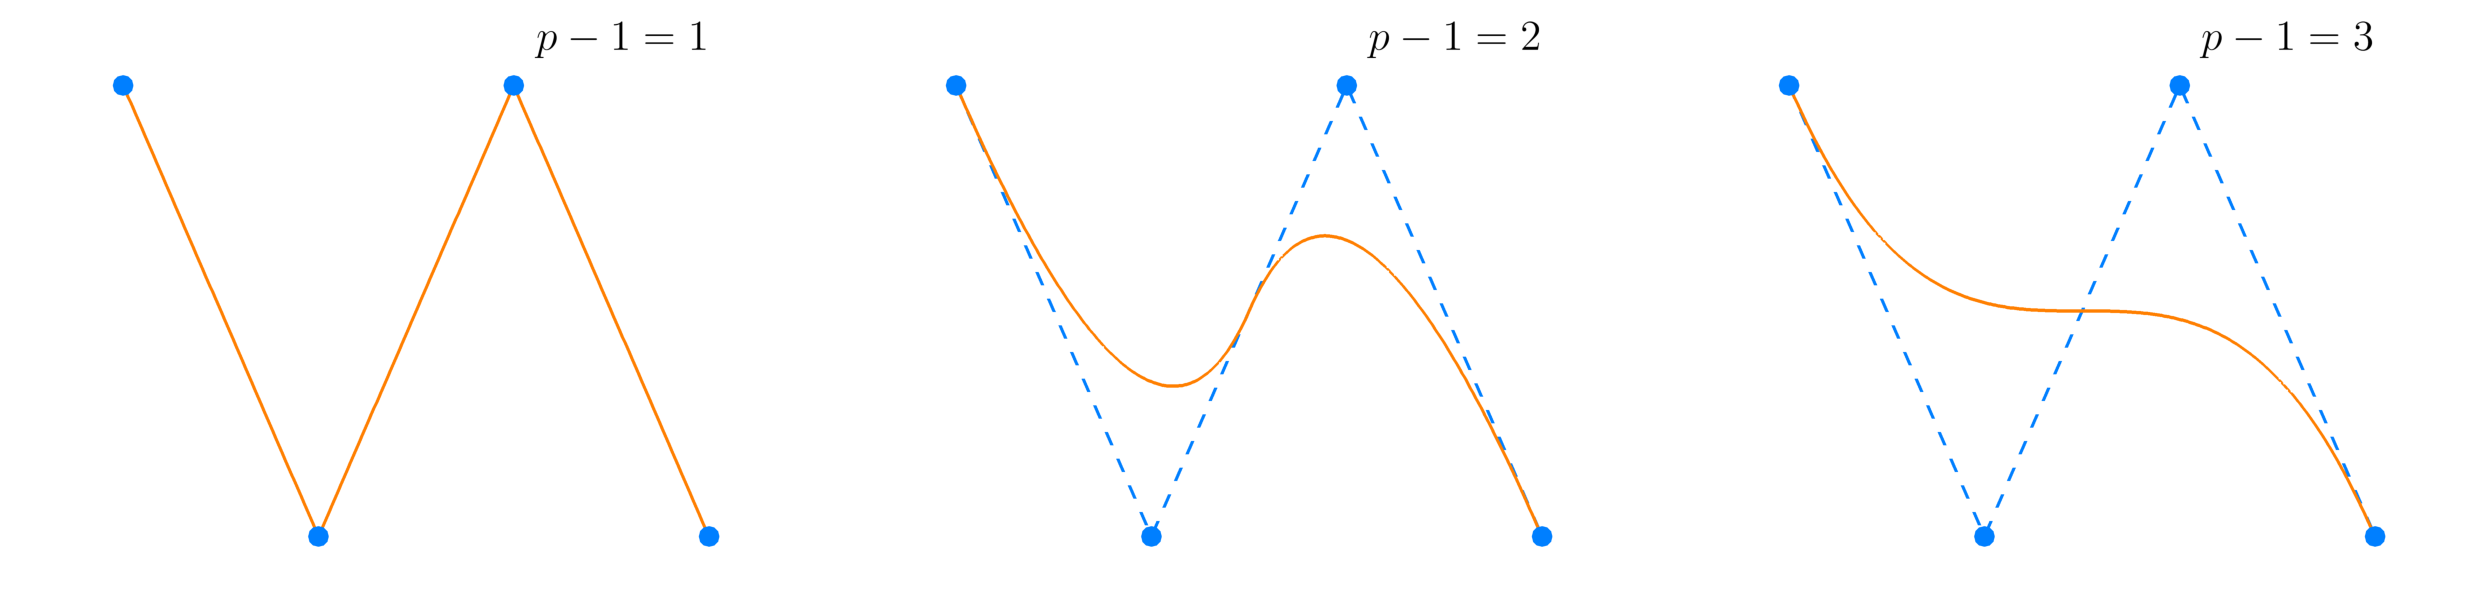
\includegraphics[width=\textwidth]{../tec/nurbsCurve/nurbsCurve.png}
		\caption{A set of control points and three NURBS curves of different degrees.}
	\end{figure}

	Now that we have defined B-spline curves and NURBS curves, we can define B-spline surfaces and NURBS surfaces in a similar manner. To do this, we require a grid of knots represented by two knot sequences $(u_m)_{m=-\infty}^{\infty}$ and $(v_m)_{m=-\infty}^{\infty}$ which satisfy the same conditions as $(t_m)$ did before. Instead of a one-dimensional set of control points, the surface definition relies on a two-dimensional set of control points.

	\begin{definition}
		A \emph{B-spline surface} $S_P(u,v)$ of degree $(p-1, q-1)$ over a set of control points $P = \{P_{i,j} : (i,j) \in \{0,1,...,n_u\} \times \{0,1,...,n_v\}\} \subset \mathbb{R}^d$ on the knot grid $(u_m), (v_m)$ is defined as
			$$ S_P(u,v) = \sum_{k_u=0}^{n_u} \sum_{k_v=0}^{n_v} N_{p,k_u}(u) N_{q,k_v}(v) P_{k_u,k_v},$$
		where $N_{p,k_u}(u) := N_{p,k_u}^{(u_m)}(u)$ and $N_{q,k_v}(v) := N_{q,k_v}^{(v_m)}(v)$.
	\end{definition}

	\begin{definition}
		A \emph{NURBS surface} $C_P(u,v)$ of degree $(p-1, q-1)$ over a set of control points $P = \{P_{i,j} : (i,j) \in \{0,1,...,n_u\} \times \{0,1,...,n_v\}\} \subset \mathbb{R}^d$, the control weights $w = \{w_{i,j} : (i,j) \in \{0,1,...,n_u\} \times \{0,1,...,n_v\}\} \subset \mathbb{R}$ and the knot grid $(u_m), (v_m)$ is defined as
			$$ C_P(u,v) = \frac {\sum_{k_u=0}^{n_u} \sum_{k_v=0}^{n_v} N_{p,k_u}(u) N_{q,k_v}(v) w_{k_u, k_v} P_{k_u,k_v}}{\sum_{k_u=0}^{n_u} \sum_{k_v=0}^{n_v} N_{p,k_u}(u) N_{q,k_v}(v) w_{k_u, k_v}},$$
		where $N_{p,k_u}(u) := N_{p,k_u}^{(u_m)}(u)$ and $N_{q,k_v}(v) := N_{q,k_v}^{(v_m)}(v)$.
	\end{definition}

	\begin{remark}
		As with NURBS curve, we have the analogous result
			$$ C_P(u,v) = \Phi^\dagger ({S_{\Phi_w(P)}(u,v)}) $$
		for NURBS surfaces, which also yields the same calculation strategy.
	\end{remark}

	\begin{figure}[H]
		\centering
		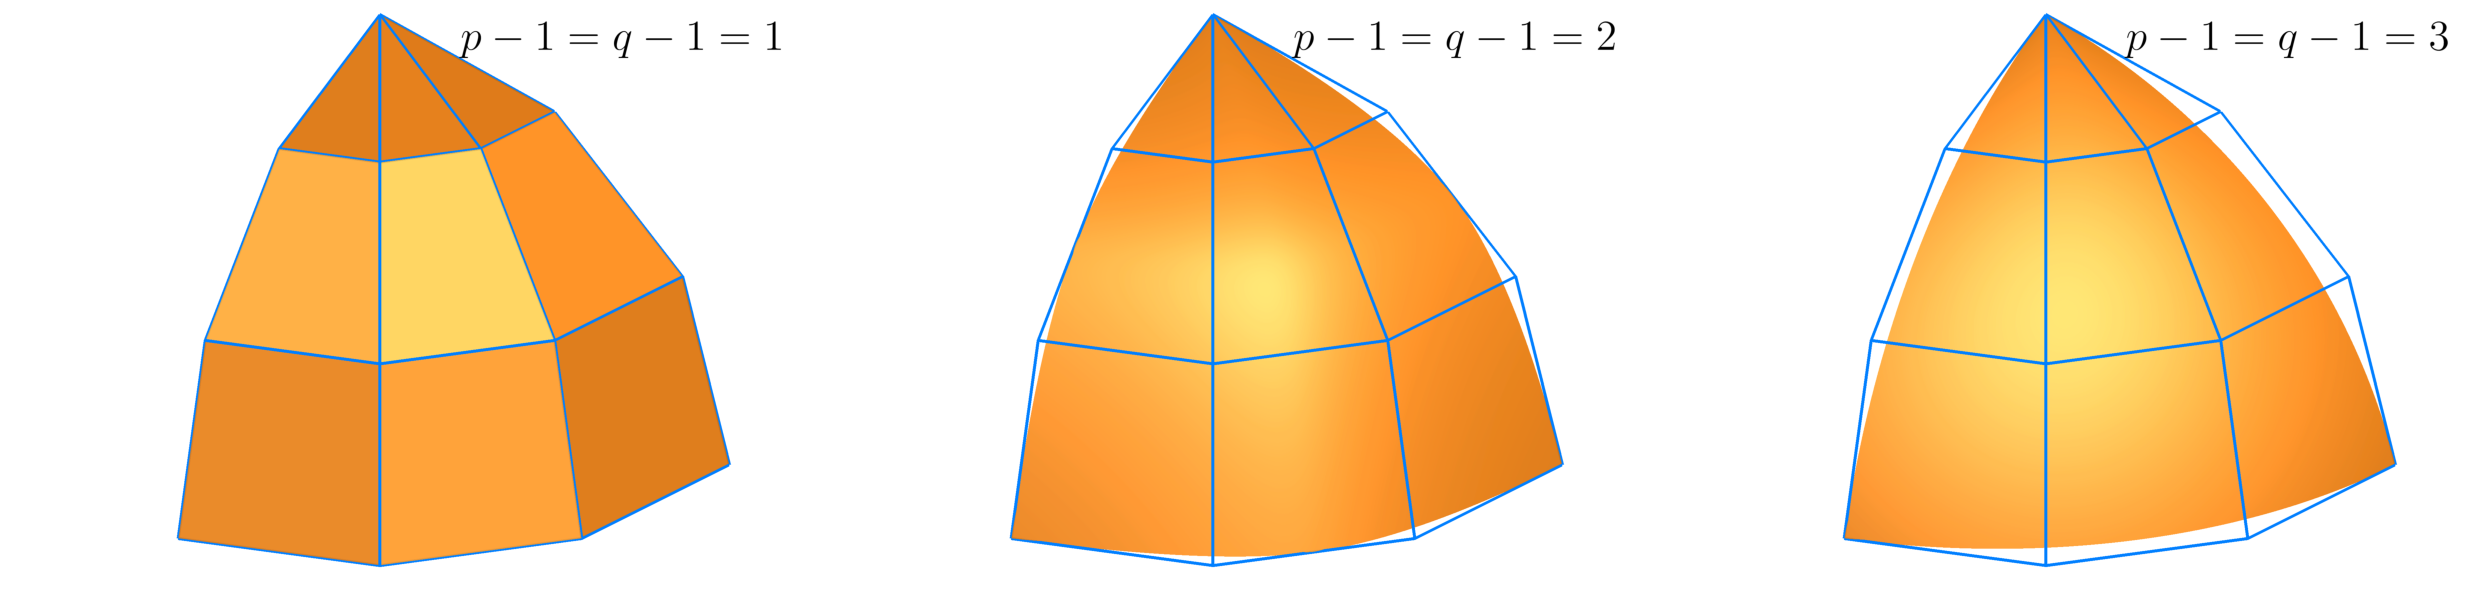
\includegraphics[width=\textwidth]{../tec/nurbsSurface/nurbsSurface.png}
		\caption{A set of control points and three NURBS surfaces of different degrees.}
	\end{figure}

	The notion of the knot sequence $(t_m)$ is commonly computationally simplified to that of a knot vector $\tau$, since $\tau$ only contains a finite number of elements. For our purposes, we let
		$$\tau = (\underbrace {t_0, ..., t_{p-1}}_{= 0}, t_p, ..., t_n, \underbrace{t_{n+1}, ..., t_{n+p}}_{= 1}),$$
	where $t_k = 0$ for $k \in \{0,...,p-1\}$ and $t_k = 1$ for $k \in \{n+1, ..., n+p\}$. We still require the monotonicity property $t_k \leq t_{k+1}$ for all $k \in \{0, ..., n+p\}$.

\subsection{De Boor's Algorithm}
	To efficiently calculate points on a B-spline object, Carl-Wilhelm Reinhold de Boor devised an efficient algorithm, the construction of which demonstrates its correctness. Together with the embedding $\Phi_w$ and the projection $\Phi^\dagger$ from the Remark for Definition \ref{def:nurbs}, this algorithm can also be used to calculate points on a NURBS object.

	Let $P = \{P_0, P_1, ..., P_n\}$ be a set of control points, $(t_m)$ a knot sequence and $p-1$ the degree of the B-spline curve $S(t)$. Then by the Cox-de-Boor recursion formula, we find
	\begin{align*}
		S(t) 	&= \sum_{k=0}^n N_{p,k}(t) \, P_k \\
				&= \sum_{k=1}^n \omega_{p-1,k}(t) \, N_{p-1, k}(t) \, P_k  \; + \; \sum_{k=0}^n \left( 1-\omega_{p-1,k+1}(t) \right) \, N_{p-1, k+1}(t) \, P_k.
	\end{align*}
	Shifting the summation index in the second sum, we can summarize the two sums0 as
	\begin{align*} 
		S(t) 	&= \sum_{k=1}^n N_{p-1, k}(t) \, \underbrace{\Big[ \omega_{p-1,k}(t) \, P_k  \, + \, \left( 1-\omega_{p-1,k}(t) \right) \, P_{k-1} \Big]}_{=: P_k^{(1)}(t)} \\
				&= \sum_{k=1}^n N_{p-1, k}(t) \, P_k^{(1)}(t).
	\end{align*}
	Recursively defining
	\begin{equation}\label{eq:debooriteration}
		P^{(j)}_k(t) := \begin{cases}
			\omega_{p-j, k} \, P^{(j-1)}_k(t) \, + \, (1-\omega_{p-j, k}) \, P^{(j-1)}_{k-1}(t) 	&\text{if } j > 0,\\
			P_k 																					&\text{else},
		\end{cases}
	\end{equation}
	we can repeat this process up to $p-2$ more times, finding
	$$ S(t) = \sum_{k=p-1}^n N_{1, k}(t) \, P^{(p-1)}_k(t) = P^{(p-1)}_l(t)$$
	for $t \in [t_l, t_{l+1})$. We can thus use the recursive definition in Equation (\ref{eq:debooriteration}) as the key step of our algorithm to compute $S(t)$. It becomes apparent that the points calculated on a B-spline curve are in fact also a cumultated convex combination of control points, just as it is the case with Bézier curves. As zero-values for $\omega_{i,j}$ (or $1-\omega_{i,j}$) can be completely omitted by counting how often the $t$ occurs in the knot vector, we arrive at the following algorithm:

	\begin{algorithm}[H]
		\begin{algorithmic}[1]
			\Input
				\Desc{$P = \{P_0, P_1, ..., P_n\}$}{set of control points of the B-spline curve}
				\Desc{$\tau = (t_0, t_1, ..., t_{n+p})$}{knot vector of the B-spline curve}
				\Desc{$p-1$}{degree of the B-spline curve}
				\Desc{$t \in [t_0, t_{n+p})$}{real number}
			\EndInput
			\Output
				\Desc{$S_P(t)$}{the point on the B-spline curve w.r.t. to $t$}
			\EndOutput

			\caption{de Boor's algorithm for curves}\label{alg:debooralgo}
			\Procedure{deBoorCurve}{$P, p, \tau, t$}
				\State Find $l$ such that $t \in [t_l, t_{l+1})$
				\State Let $m$ be the multiplicity of $t$ in the knot vector $\tau$
				\State $P^{(0)} \gets P$

				\For {$j = 1, 2, ..., p-m-1$}
					\For {$k = l-p+j+1, ..., l-m$}
						\State $\omega_{p-j,k} \gets \frac{t-t_k}{t_{k+p-j} - t_k}$
						\State $P^{(j)}_k \gets (1-\omega_{p-j,k}) \cdot P^{(j-1)}_{k-1} + \omega_{p-j,k} \cdot P^{(j-1)}_k$
					\EndFor
				\EndFor

				\State \Return $P^{(p-m-1)}_{l-m} = S_P(t)$
			\EndProcedure
		\end{algorithmic}
	\end{algorithm}

	\begin{figure}[H]
		\centering
		\begin{subfigure}{0.49\textwidth}
			\begin{tikzpicture}
				\def\dx{65pt}
				\def\dy{30pt}

				\pgfmathsetmacro{\degree}{3}

				% Make nodes
				\setcounter{i}{0}
				\setcounter{j}{0}

				\node (\arabic{i}) at (0,0) {$P^{(\degree)}_l$};
				\stepcounter{i}

				\foreach \x in {1, ..., \degree} {
					\pgfmathsetmacro{\xstep}{\x-2}

					\setcounter{j}{0}
					\foreach \y in {\x, \xstep, ..., -\x} {

						\ifthenelse{\value{j}>0} {
							\node (\arabic{i}) at (\x*\dx, \y*\dy) {$P^{(\pgfmathint{\degree-\x}\pgfmathresult)}_{l-\arabic{j}}$};
						}
						{
							\node (\arabic{i}) at (\x*\dx, \y*\dy) {$P^{(\pgfmathint{\degree-\x}\pgfmathresult)}_l$};
						}
						\stepcounter{i}
						\stepcounter{j}
					}
				}
				
				% Make arrows
				\setcounter{z}{0}
				\setcounter{a}{0}
				\setcounter{b}{0}
				\pgfmathsetmacro{\maxx}{\degree}
				\foreach \x in {1,...,\degree}{
					\foreach \y in {1,...,\x}{
						
						\setcounter{a}{\arabic{z}}
						\addtocounter{a}{\x}

						\setcounter{b}{\arabic{z}}
						\addtocounter{b}{\x}
						\stepcounter{b}
						
						\ifthenelse{\y > 1} {
							\draw [<-] (\arabic{z}) -- (\arabic{b}) node[above, midway, sloped] {\scriptsize $1-\omega_{\pgfmathint{\x}\pgfmathresult, l-\pgfmathint{\y-1}\pgfmathresult}$};
							\draw [<-] (\arabic{z}) -- (\arabic{a}) node[above, midway, sloped] {\scriptsize $\omega_{\pgfmathint{\x}\pgfmathresult, l-\pgfmathint{\y-1}\pgfmathresult}$};
						}
						{
							\draw [<-] (\arabic{z}) -- (\arabic{b}) node[above, midway, sloped] {\scriptsize $1-\omega_{\pgfmathint{\x}\pgfmathresult, l}$};
							\draw [<-] (\arabic{z}) -- (\arabic{a}) node[above, midway, sloped] {\scriptsize $\omega_{\pgfmathint{\x}\pgfmathresult, l}$};
						}

						\stepcounter{z}
					}
				}
			\end{tikzpicture}
			\caption{Visualization of de Boor's algorithm on a curve $S_P(t)$ with degree $3$, where $t$ does not appear in the knot vector $\tau$ (in other words, $m=0$.}
		\end{subfigure}
		\hfill
		\begin{subfigure}{0.49\textwidth}
			\centering
			\includesvg[width=0.99\textwidth]{../python/nurbsCurveExample}
			\caption{Degree $3$ NURBS curve $\Phi^\dagger(S_{\Phi_w(P)}(t))$  for different values of a single entry of the control weight vector $w$.}
		\end{subfigure}
		\caption{Calculating points on a NURBS curve.}
		\label{fig:debooralgo}
	\end{figure}

	To calculate one point on the B-spline curve $S_P$ of degree $p$, we require at most $\frac{p^2-p}{2}$ vector additions and $p^2-p$ scalar multiplications, which is quite similar to what we found for Bézier curves. However, we also need to calculate $\omega_{j,k}$ at every step, which in total sums up to $p^2-p$ real additions and $\frac{p^2-p}{2}$ real multiplications.

	By writing the definition of the B-spline surface as
		$$ S_P(u,v) = \sum_{k_u=0}^{n_u} \sum_{k_v=0}^{n_v} N_{p,k_u}(u) N_{q,k_v}(v) P_{k_u,k_v} = \sum_{k_u=0}^{n_u} N_{p,k_u}(u) \underbrace{\left( \sum_{k_v=0}^{n_v} N_{q,k_v}(v) P_{k_u,k_v} \right)}_{:= \, q_{k_u}(v)},$$
	we can observe that Algorithm \ref{alg:debooralgo} can be utilized to calculate points on B-splines surfaces. To do this, we run the de Boor's algorithm to calculate $q_{k_u}(v)$.

	\begin{algorithm}[H]
		\begin{algorithmic}[1]
			\Input
				\Desc{$P = \{P_{i,j}\}$}{set of control points with $n_1 \cdot n_2$ elements}
				\Desc{$\tau_u = (u_0, u_1, ..., u_{n_u+p})$}{first knot vector of the B-spline curve}
				\Desc{$\tau_v = (v_0, v_1, ..., v_{n_v+q})$}{second knot vector of the B-spline curve}
				\Desc{$p-1$}{first degree of the B-spline curve}
				\Desc{$q-1$}{second degree of the B-spline curve}
				\Desc{$u \in [u_0, u_{n_u+p})$}{first real number}
				\Desc{$v \in [v_0, v_{n_v+q})$}{second real number}
			\EndInput
			\Output
				\Desc{$S_P(u,v)$}{the point on the B-spline curve w.r.t. to $u, v$}
			\EndOutput

			\caption{de Boor's algorithm for surfaces}\label{alg:debooralgosurf}
			\Procedure{deBoorSurface}{$P, p, q, \tau_u, \tau_v, u, v$}
				\State Find $l$ such that $u \in [u_{l}, u_{l+1})$
				\State Let $m$ be the multiplicity of $u$ in the knot vector $\tau_u$

				\For {$k = l-p+1, , ..., l-m-1$}
					\State $Q_k \gets \text{deBoorCurve}(P_{k,\cdot}, q, \tau_v, v)$	
				\EndFor
				
				\State \Return $\text{deBoorCurve}(Q, p, \tau_u, u)$
			\EndProcedure
		\end{algorithmic}
	\end{algorithm}

	Similarly to the Remark under Definition \ref{def:nurbs}, we can use Algorithm \ref{alg:debooralgosurf} to calculate points on NURBS surfaces by employing the projection map $\Phi_w$ and the projection map $\Phi^\dagger$.

\subsection{Properties}
	In this section, we will see that B-spline curves and NURBS curves share some (although not all) useful properties with Bézier curves.

	\begin{theorem}
		Let $S_P$ be a B-spline curve and let $C_P$ be a NURBS curve. Then $S_P(0) = P_0$ and $S_P(1) = P_n$ and therefore $C_P(0) = P_0$ and $C_P(1) = P_n$.
	\end{theorem}
	\begin{proof}
		By using Algorithm \ref{alg:debooralgo}, we have $m = p$ and return $P_l$ without calculation, which is $P_0$ in the case of $t = 0$ and $P_n$ in the case of $t = 1$. Then by $C_P(t) = \Phi^\dagger(S_{\Phi_w(P)}(t))$, we have $C_P(0) = \Phi^\dagger\Phi_w(P_0) = P_0$ and $C_P(1) = \Phi^\dagger\Phi_w(P_n) = P_n$.
	\end{proof}

	\begin{theorem}
		Let $T \in \mathbb{R}^{d \times d}$. Let $S_P$ be a B-spline curve or surface and $C_P$ a NURBS curve or surface. Then $S_{TP} = TS_P$ and $C_{TP} = TC_P$.
	\end{theorem}
	\begin{proof}
		By linearity of $T$ we can compute
			$$S_{TP}(t) = \sum_{k=0}^{n} N_{p,k}(t) TP_k = T \left( \sum_{k=0}^{n} N_{p,k}(t) P_k \right) = TS_P(t)$$
		for B-spline curves and
			$$C_{TP}(t) = \frac{\sum_{k=0}^n N_{p,k}(t) w_k TP_k}{\sum_{k=0}^n N_{p,k}(t) w_k} = T \left( \frac{\sum_{k=0}^n N_{p,k}(t) w_k P_k}{\sum_{k=0}^n N_{p,k}(t) w_k} \right) = TC_P(t)$$
		for NURBS curves.
		Similarly, we can compute
			$$ S_{TP}(u,v) = \sum_{k_u=0}^{n_u} \sum_{k_v=0}^{n_v} N_{p,k_u}(u) N_{q,k_v}(v) TP_{k_u,k_v} = TS_P(u,v)$$
		for B-spline surfaces and
			$$ C_{TP}(u,v) = \frac {\sum_{k_u=0}^{n_u} \sum_{k_v=0}^{n_v} N_{p,k_u}(u) N_{q,k_v}(v) w_{k_u, k_v} TP_{k_u,k_v}}{\sum_{k_u=0}^{n_u} \sum_{k_v=0}^{n_v} N_{p,k_u}(u) N_{q,k_v}(v) w_{k_u, k_v}} = TC_P(u,v) $$
		for NURBS surfaces.
	\end{proof}

	\begin{theorem}
		A B-spline curve or surface $S_P$ lies in the convex hull of its control points $P$.
	\end{theorem}
	\begin{proof}
		Using Equation (\ref{eq:debooriteration}), we can see that every iteration of Algorithm \ref{alg:debooralgo} produces a set of points which all lie in the convex hull of the last iteration. Therefore, $S_P(t) = P^{(p-1)}_l$ lies in the convex hull of $P^{(0)}$ for all $l$.
	\end{proof}
	\begin{remark}
		This theorem does not hold for NURBS curves and surfaces $C_P$.
	\end{remark}

	For a given degree $p$, B-spline and NURBS curves can have any number $n > p+1$ of control points. This makes them a much more flexible tool than their Bézier counterpart. Yet Bézier, B-splines and NURBS curves still share a lot of nice properties, which makes them, once implemented, easy to use.

\section{Common Methods on Curves and Surfaces}
	In this section, the most important tools of CoolingGen are presented. The modification of NURBS objects through their control points may be simple, but common and useful operations that are imperative for CAD are, unfortunately, not as simple. Such operations include the calculation of intersection points of NURBS objects, the projection of an arbitrary point in space onto a NURBS object and the construction of so called offset curves and fillets.

	This comes down to the fact that many of the problem statements are (generally) non-convex minimization problems. However, these problems can often be greatly simplified by asserting properties of underlying geometric patterns that arise in specific procedures.

\subsection{Point Projection}\label{subsec:pointproj}
	Let $\gamma(t) \subset \mathbb{R}^d$ a parametric curve, $t \in [0,1]$, and let $Q \in \mathbb{R}^d$ a point.
	We want to find an element in the set
		$$T^* := \underset{t\in[0,1]}{\arg\min} \; D(\gamma(t), Q), $$
	where $D(\cdot, \cdot)$ is the Euclidean distance between two points. Notice that 
		$$\underset{t\in[0,1]}{\min} \; D(\gamma(t), Q) = D(\gamma(t^*), Q), $$
	is the distance between the curve $\gamma$ and the point $Q$, and is constant for all $t^* \in T^*$.
	We call $T^*$ the set of projection parameters for the point $Q$ onto the curve $\gamma$.

	\begin{figure}[H]
		\centering
		\includesvg[width=0.7\textwidth]{../python/pointInversionFigure}
		\caption{Point projection. Each blue point on the orange curve is the projection of the point connected to it with a dotted line.}
		\label{fig:pointinversion}
	\end{figure}

	\begin{definition}
		The distance between a parametric curve $\gamma(t) \subset \mathbb{R}^d$ with $t \in [0,1]$ and a point $Q \in \mathbb{R}^d$ is given by
			$$D(Q, \gamma) := D(\gamma, Q) := \underset{t \in [0,1]}{\min} \; D(\gamma(t), Q).$$
	\end{definition}

	\begin{remark}
		If $D(Q, \gamma) = 0$, then by the point-separating property of the Euclidean norm, $Q$ lies on the curve $\gamma$. This special case, in which the point $Q$ lies on the curve $\gamma(t)$, will be handled later. In general, the projection of a point is not necessarily unique. If we consider, for example, the curve $\gamma(t) = (\sin 2\pi t, \cos 2\pi t)$ with $t \in [0,1]$ and $Q = (0,0)$, the set of projection parameters $T^*$ is equal to the whole domain of definition $[0,1]$.
	\end{remark}

	Minimizing distance functions for general curves is a problem that is hard to solve. We therefore make some assumptions about the point-curve distance function $\phi(t) := D(\gamma(t), Q)$ that we are going to minimize in order to find one target parameter $t^* \in T^*$. If $\phi$ is convex and two times differentiable, then this problem can be solved iteratively by Newton's method. For an initial guess $t^{(0)}$ close to a target parameter $t^* \in T^*$ we use the iteration
		$$ t^{(n+1)} = t^{(n)} - \frac {\phi'(t^{(n)})}{\phi''(t^{(n)})}. $$
	Here, $\phi'(t)$ is the derivative of $\phi(t)$ with respect to $t$, which for a small value of $\epsilon > 0$ can be approximated by the central difference quotient
		\begin{equation}
			\phi'(t) \approx \frac{\phi(t+\epsilon) - \phi(t-\epsilon)}{2\epsilon}
		\end{equation}
	for $t \in [\epsilon, 1-\epsilon]$. The expression $\phi''(t)$ is the second derivative of $\phi(t)$ with respect to $t$, which can be approximated by the difference quotient
		\begin{equation}
			\phi''(t) \approx \frac{\phi(t+\epsilon) - 2\phi(t) + \phi(t-\epsilon)}{\epsilon^2}
		\end{equation}
	for $t \in [\epsilon, 1-\epsilon]$. For $t_0 \in [0,\epsilon]$, we assign $\phi'(t_0) \approx \phi'(\epsilon)$ and $\phi''(t_0) \approx \phi''(\epsilon)$ and for $t_1 [1-\epsilon,1]$ we assign $\phi'(t_1) \approx \phi'(1-\epsilon)$ and $\phi''(t_1) \approx \phi''(1-\epsilon)$.

	However, in CoolingGen we often cannot make the assumption of differentiability or convexity of $\phi$. We therefore employ a pragmatic scheme and assume piecewise two time differentiability and piecewise convexity of $\phi$ and run Newton's method only on a small subinterval $[l,u] \subset [0,1]$.

	To find $[l,u]$, we sample the curve $\gamma(t)$ at a set of points $\{t_0, t_1, ..., t_n\}$ with $t_i = \frac{i}{n}$ and seek
		$$ m = \underset{t\in\{t_0, t_1, ..., t_n\}}{\arg\min} \phi(t). $$
	We let $l = m - \frac{1}{n}$ and $u = m + \frac{1}{n}$. Next, we can use Newton's method with the start value $m$ to find
		$$ t^* = \underset{t\in[l,u]}{\arg\min}\;\phi(t). $$
	This scheme will only converge to the global minimum of $\phi$ for large enough $n \in \mathbb{N}$.

	We describe the procedure in pseudo-code. The start and boundary value search is described by the following algorithm.
	\begin{algorithm}[H]
		\begin{algorithmic}[1]
			\Input
				\Desc{$N$}{number of samples for initial value search}
			\EndInput
			
			\caption{Start value search}

			\Procedure{findPointProjectionInitValues}{$\gamma, Q$}
				\State $m \gets 0$
				\For {$k = 1,...,N$}
					\State $t \gets \frac{k}{N}$
					\If {$D(Q, \gamma(m)) > D(Q, \gamma(t))$}
						$m \gets t$
					\EndIf
				\EndFor

				\State \Return $m-\frac{1}{N}, m+\frac{1}{N}, m$
			\EndProcedure
		\end{algorithmic}
	\end{algorithm}
	Using the start and boundary values, we apply Newton's method for $M$ iterations to find our target value, which is returned upon completion.
	\begin{algorithm}[H]
		\begin{algorithmic}[1]
			\Input
				\Desc{$M$}{number of iterations}
				\Desc{$\epsilon > 0$}{differentiation step (small)}
			\EndInput

			\caption{Point Projection}\label{alg:pointinversion}
			\Procedure{pointProjection}{$\gamma, Q$}
				\State $l, u, m \gets \text{findPointProjectionInitValues}(\gamma, Q)$
				\State $t \gets m$

				\For {$k = 1, 2,..., M$}
					\State $t_+ \gets t + \epsilon$ and $t_- \gets t - \epsilon$
					\State $\phi \gets D(\gamma(t), Q)$
					\State $\phi_+ \gets D(\gamma(t_+), Q)$ and $\phi_- \gets D(\gamma(t_-), Q)$

					\State $\phi' \gets \frac{\phi_+ - \phi_-}{2\epsilon}$
					\State $\phi'' \gets \frac{\phi_+ - 2\phi + \phi_-}{\epsilon^2}$
					
					\State $t \gets t - \frac{\phi'}{\phi''}$
					\If {$t < l$} $t \gets l$ \EndIf
					\If {$t > u$} $t \gets u$ \EndIf

				\EndFor

				\State \Return $t$
			\EndProcedure
		\end{algorithmic}
	\end{algorithm}

	If the curve $\gamma(t)$ does not satisfy the aforementioned assumptions, then we might still be able to find $t^*$ by applying the start value search scheme iteratively on the domain of $\gamma(t)$ to find smaller intervals $[l,u]$ if $\gamma(t)$ is at least continuous. Continuity of curves can safely be assumed all throughout CoolingGen.

	We now treat the special case that the minimum target distance is equal to zero, in which case $Q$ lies on the curve $\gamma(t)$.
	\begin{theorem}
		Let $\gamma(t) \subset \mathbb{R}^d$ be a curve, $t \in [0,1]$ and let $Q \in \mathbb{R}^d$. If $\gamma$ has no self-intersections and
			$$\underset{t\in[0,1]}{\min} \; D(\gamma(t), Q) = 0$$
		then $T^*$ is a single element set.
	\end{theorem}
	\begin{proof}
		If $\gamma$ has no self-intersections, then no two parameters of $\gamma$ will map onto the same point. Therefore, $\gamma$ is injective. We know $t^*$ exists such that $D(\gamma(t^*), Q) = 0$, which by the point-separating property of the Euclidean norm is equivalent to $Q = \gamma(t^*)$. By injectivity, this $t^*$ is unique.
	\end{proof}

	If the target distance is zero and $\gamma$ is a NURBS curve, we can observe that the devised scheme is the inversion of de Boor's algorithm (Algorithm \ref{alg:debooralgo}), that will return the input parameter that fits the point $Q$. This justifies the name \emph{point inversion} for this special case.

	Using these principles, we can also project (or invert) a point $Q \in \mathbb{R}^d$ on a parametric surface $\beta(u,v)$ with $u,v \in [0,1]$ by generalizing the presented methods.
	In this case, the distance function we want to minimize is 
		$$ \phi(u,v) := D(\beta(u,v), Q)$$
	We once again use the start value search. We let $u_i = \frac{i}{n_u}, v_j = \frac{j}{n_v}$ for $i \in \{0, ..., n_u\}, j \in \{0,..., n_v\}$ and $n_u, n_v \in \mathbb{N}$. Then we seek
		$$ m_u, m_v = \underset{(u,v)\in\{u_0, ..., u_n\} \times \{v_0, ..., v_n\}}{\arg\min} \phi(u,v), $$
	where $\phi(u,v) := D(\beta(u,v), Q)$. We use Newton's method only on the subset
		$$  M = [m_u - \frac{1}{n_u}, m_u + \frac{1}{n_u}] \times [m_v - \frac{1}{n_v}, m_v + \frac{1}{n_v}] \subset [0,1]^2, $$
	which in this case for each iteration yields a linear system of equations
		$$ 	
			H_\phi
			\left(
					u^{(k)},
					v^{(k)}
			\right)
			\cdot
			\begin{pmatrix}
				u^{(k+1)} - u^{(k)} \\
				v^{(k+1)} - v^{(k)} 
			\end{pmatrix} 
			=
			-\nabla \phi
			\left(
					u^{(k)},
					v^{(k)}
			\right),
		$$
	where $H_\phi(u,v)$ is the Hessian of $\phi$ and $\nabla \phi(u,v)$ is the gradient of $\phi$. These differentials can once again be approximated by finite differences. If $H_\phi(u,v)$ and $\nabla \phi(u,v)$ do not exist for some $(u,v)$ in the set $M$, then we can once again iteratively apply the start value search to find smaller subsets of $M$ to calculate some $(u^*, v^*)$ in the set of projection parameters for the point $Q$.

\subsection{Intersection of a Ray and a Curve in 2D}\label{subsec:raymarching}
	\begin{definition}
		A \emph{ray} with support vector $A \in \mathbb{R}^d$ and direction vector $B \in \mathbb{R}^d$ is given by the set of points
			\begin{equation*}
				\hat R_{A,B} = \{A + tB \;:\; t \in \mathbb{R},\; t \geq 0\}.
			\end{equation*}
		The dependence of a point on the ray on the real parameter $t$ motivates the description of this set as a map
			$$R_{A,B}: \mathbb{R} \rightarrow \mathbb{R}^d,\;\; t \mapsto A+tB.$$
		which yields the equation $\hat R_{A,B} = R_{A,B}([0,\infty))$.
	\end{definition}

	In this section, we want to find an algorithm that intersects a curve $\gamma(t)$ with $t \in [0, 1]$ with a ray $R_{A,B}(s)$ with $s \in [0, \infty)$. Generally, the intersection of these two sets can be written as
		$$I = \gamma([0,1]) \cap R_{A,B}([0,\infty)).$$
	The algorithm presented will return only up to one element in that set, specifically the one corresponding to the lowest value of the ray parameter $s$. If however $I = \emptyset$, then no element will be returned.

	\begin{definition}
		Let $R_{A,B}$ a ray and $\gamma(t)$ a curve. Then the ray-curve-distance w.r.t $R_{A,B}$ and $\gamma$ is defined as
			$$ D(R_{A,B}, \gamma) := D(\gamma, R_{A,B}) := \underset{s\in[0,\infty)}{\min} \; D(\gamma, R_{A,B}(s))$$
	\end{definition}
	
	\begin{definition}\label{def:raycollisionparameter}
		Let $R_{A,B}(s)$ a ray and $\gamma(t)$ a curve. If a solution to 
			$$\underset{s\in[0,\infty)}{\min} \; s \quad \text{subject to} \quad D(\gamma, R_{A,B}(s)) = 0$$
		exists, then it is called \emph{collision parameter} of $R_{A,B}$ w.r.t. $\gamma$.
	\end{definition}

	We define the return value of our algorithm as the one element set given by
		$$ I_{\min} := 
			\begin{cases}
				\{R_{A,B}(s^*)\} 	&\text{if } D(R_{A,B}(s^*), \gamma) \leq \epsilon, \\
				\emptyset			&\text{otherwise,}	
			\end{cases}
		$$
	where the absolute tolerance $\epsilon > 0$ is close to $0$ and $s^*$ is an approximation of the collision parameter of $R_{A,B}$ w.r.t. $\gamma$. If $I_{\min} \neq \emptyset$, then we refer to the element in $I_{\min}$ as \emph{collision point}.

	\begin{remark}
		Why is the notion of the collision point of interest? To exemplify the prospect of our algorithm, imagine the following scenario: Let there be a reflective interface represented by a curve $\gamma$ and a beam of light represented by a ray $R_{A,B}$. Then our model suggests the equivalence of the physical point of reflection and the collision point of the ray with respect to the curve.
	\end{remark}

	We can find the approximation $s^*$ of the collision parameter by using a common CAD scheme called \emph{ray marching}, in which we traverse the ray $R_{A,B}$ by a small distance increments $s$ until we achieve collision with the curve $\gamma$. How do we choose the optimal value for $s$? The idea is the following: Using the point projection algorithm, we can calculate the \emph{safe distance} $s$ of the point $A$ on the ray to the curve $\gamma$. Then we can easily construct a point $P$ that fulfills $D(A,P) = s$ and lies on the ray $R_{A,B}$ by 
		$$ P := A+s\frac{B}{||B||}.$$
	Now there are only two possibilities: Either $P$ lies within the $\epsilon$-ball of the collision point, or the line segment $\overline{AP} \subset R_{A,B}([0,\infty))$ has at least $\epsilon$ distance to $\gamma$. In the first case, we can return $\{P\}$. In the second case, we can repeat the procedure on the set 
		$$ R_{A,B}([0,\infty)) \setminus \overline{AP} = R_{A,B}([s,\infty)) = R_{P,B}([0,\infty)).$$
	If after a certain amount of iterations $N$ the algorithm does not converge to a point which lies within the $\epsilon$-ball of the collision point, we return $\emptyset$.

	\begin{figure}[H]
		\centering
		\includesvg[width=0.9\textwidth]{../python/rayMarching}
		\caption{Ray marching.}
		\label{fig:raymarchingvis}
	\end{figure}

	Figure \ref{fig:raymarchingvis} describes ray marching visually. At each iteration, a new safe distance $s$ (depicted as green circle radii) along the ray is calculated. The ray is traversed using $s$ as step size (to achieve the points depicted in green) until the safe distance falls below the absolute tolerance $\epsilon$. The resulting point, depicted in purple, is close to the collision point. The implementation of ray marching algorithm given a point projection algorithm proves to be relatively simple.

	\begin{algorithm}[H]
		\begin{algorithmic}[1]

			\caption{Ray Marching}\label{alg:raymarching}
			\Procedure{intersectCurveRay}{$\gamma, A, B$}
				\State $B \gets \frac{B}{||B||}, s \gets 0, P \gets A$
				\For {$k = 1, 2,..., N$}
					\State $s \gets D(\gamma(\text{pointProjection}(\gamma, P)), P)$
					\State $P \gets P + sB$
					\If {$s < \epsilon$}
						\State \Return $\{P\}$
					\EndIf
				\EndFor

				\State \Return $\emptyset$
			\EndProcedure
		\end{algorithmic}
	\end{algorithm}

	Using the point projection algorithm for surfaces (instead of the point projection algorithm for curves) to find the distance between a point and a surface, we can generalize this algorithm to find the intersection of a ray and a surface.

\subsection{Intersecting Two Curves in 2D}
	In order to trim curves at intersection points, we require the pair of parameters at which two curves intersect. Let $\gamma_1(s)$ and $\gamma_2(t)$ be two continuous curves in $\mathbb{R}^2$ with $s,t \in [0,1]$ which intersect at finitely many points at most. In this section, we seek for the set of parameters at which these curves intersect.

	\begin{definition}
		The distance between two curves $\gamma_1, \gamma_2$ is defined as
			$$ D(\gamma_1, \gamma_2) := \min_{(s,t) \in [0,1]^2} D(\gamma_1(s), \gamma_2(t)).$$
	\end{definition}

	Similarly to the prior sections, our goal is to minimize a distance function $D(\gamma_1(s), \gamma_2(t))$. In this case, we will employ a pragmatic scheme that uses a piecewise linear approximation of the curve, in which finding intersections is comparably simple and involves finding the intersection of a number of line segments.

	\begin{definition}
		The intersection parameter set of two continuous curves $\gamma_1$ and $\gamma_2$ is defined as
				$$ I(\gamma_1, \gamma_2) := \{(s,t) \in [0,1]^2 : \gamma_1(s) = \gamma_2(t)\}.$$
		Notice that $\gamma_1([0,1]) \cap \gamma_2([0,1]) = \emptyset$ if and only if $I(\gamma_1, \gamma_2) = \emptyset$.
	\end{definition}

	\begin{figure}[H]
		\centering
		\includesvg[width=\textwidth]{../python/curveIntersectionConnectedness}
		\caption{In (A) we have $|I(\gamma_1, \gamma_2)| < \infty$, whereas in (B) we have $|I(\gamma_1, \gamma_2)| = \infty$.}
		\label{fig:curveIntersectionConnectedness}
	\end{figure}

	For the use with CoolingGen, our goal is to find the set $I(\gamma_1, \gamma_2)$ in case of $|I(\gamma_1, \gamma_2)| < \infty$ (see Figure \ref{fig:curveIntersectionConnectedness}).

	\begin{definition}\label{def:linesegdef}
		The line segment between the points $A_s = (A_{s_x}, A_{s_y})^T$ and $A_e = (A_{e_x}, A_{e_y})^T$ is defined as the set
			$$ \overline{A_s A_e} := \{(1-t)A_s + tA_e : t \in [0,1]\}. $$
		The dependence of a point on the line segment on the real parameter $t$ motivates the description of this set as a map
			$$ L_A : \mathbb{R} \rightarrow \mathbb{R}^d, \quad t \mapsto (1-t)A_s + tA_e,$$
		which yields the equation $\overline{A_s A_e} = L_A([0,1])$. Notice that given the definition of the direction vector $A_d := A_e - A_s = (A_{d_x}, A_{d_y})$, we can write
			$$ L_A(t) = A_s + tA_d.$$
	\end{definition}
	
	We write the derivative of a curve $\gamma(t)$ as $\nabla \gamma(t) := \gamma'(t)$. The key idea of our algorithm is described by the following theorem.

	\begin{theorem}\label{thm:parallelintersection}
		Let $\gamma_1$ and $\gamma_2$ be two differentiable curves and let $(s^*, t^*) \in I(\gamma_1, \gamma_2) \cap (0,1)^2$. If the curve derivatives $\nabla\gamma_1(s^*)$ and $\nabla\gamma_2(t^*)$ are not parallel, then there exist neighborhoods 
			$$[s^*-\epsilon, s^*+\epsilon] \quad\text{and}\quad [t^*-\epsilon, t^*+\epsilon]$$
		around $s^*$ and $t^*$, respectively, where $\epsilon > 0$ such that the line segments
			$$\overline{\gamma_1(s^*-\epsilon) \, \gamma_1(s^*+\epsilon)} \quad\text{and}\quad \overline{\gamma_2(t^*-\epsilon) \, \gamma_2(t^*+\epsilon)}$$
		intersect. 
	\end{theorem}
	\begin{remark}
 		Suppose that the line segments $\overline{\gamma_1(s_1) \, \gamma_1(s_2)}$ and $\overline{\gamma_2(t_1) \, \gamma_2(t_2)}$ intersect. We cannot conclude that there is an intersection $(s,t) \in I(\gamma_1, \gamma_2)$ with $s \in [s_1, s_2]$ and $t \in [t_1, t_2]$. Using this theorem as core concept for our algorithm, we will need to ensure that the distance between the target curve segments is zero. In this numerical setting, it is sufficient to instead ensure
 			$$ D(\gamma_1 \domrestr_{[s_1, s_2]}, \gamma_2 \domrestr_{[t_1, t_2]}) \leq \alpha$$
 		for a sufficiently small absolute tolerance $\alpha > 0$. If this is not the case, then no intersection lies inside of $[s_1, s_2] \times [t_1, t_2]$ and every line segment intersection found within should be discarded. Here, the notation $\gamma \domrestr{M}$ for some parametric curve $\gamma$ and a subset $M \in [0,1]$ is the domain restriction of $\gamma$ onto $[a,b]$.
	\end{remark}
	
	\begin{figure}[H]
		\centering
		\includesvg[width=0.55\textwidth]{../python/linearApproxCircleIntersection}
		\caption{Two curves that intersect in a point tangentially and their linear approximations.}
		\label{fig:tangentialintersection}
	\end{figure}

	What Theorem \ref{thm:parallelintersection} and it's Remark tell us is that parallel intersection points (for example in two circular curves that intersect in exactly one point, see Figure \ref{fig:tangentialintersection}) are rarely detected by intersecting a piecewise linear approximation of the curve. In other words, if for any intersection parameter pair $(s^*, t^*) \in I(\gamma_1, \gamma_2)$ we have $\nabla \gamma_1(s^*) = \nabla \gamma_2(t^*)$, then it is likely that the intersection is not detected by the described line segment intersection scheme.
 	
	\begin{theorem}\label{thm:lineintersection}
		Let $L_A([0,1])$ and $L_B([0,1])$ be two line segments in $\mathbb{R}^2$. If the lines $L_A((-\infty,\infty))$ and $L_B((-\infty,\infty))$ are not parallel, their single intersection pointt is given by $L_A(t_A) = L_B(t_B)$, where
			\begin{equation*}\label{eq:lineintersection}
				t_A = 
				\frac {
					\det
					\begin{pmatrix}
						\Delta S_y 	& \Delta S_x		\\
						B_{d_y}	& B_{d_x}
					\end{pmatrix}
				}
				{
					\det
					\begin{pmatrix}
						B_{d_x} & B_{d_y} 	\\
						A_{d_x} & A_{d_y}
					\end{pmatrix}
				}
				\quad\text{and}\quad
				t_B =
				\frac {
					\det
					\begin{pmatrix}
						\Delta S_y 	& \Delta S_x		\\
						A_{d_y}	& A_{d_x}
					\end{pmatrix}
				}
				{
					\det
					\begin{pmatrix}
						B_{d_x} & B_{d_y} 	\\
						A_{d_x} & A_{d_y}
					\end{pmatrix}
				},
			\end{equation*}
		where $\Delta S = B_s - A_s$ and $t_A, t_B \in \mathbb{R}$. If $t_A \in [0,1] \wedge t_B \in [0,1]$, the line segments intersect in a single point.
	\end{theorem}
	
	In our algorithm we sample the curves $\gamma_1$ and $\gamma_2$ at $t_i = \frac{i}{N}$, where $i \in \{0,...,N\}$. In the next step we check for an intersection of 
		$$\overline{\gamma_1(t_i) \, \gamma(t_{i+1})} \quad\text{and}\quad \overline{\gamma_2(t_j) \, \gamma_2(t_{j+1})}$$
	for $i,j \in \{0,...,N-1\}$. For all intersection pairs $(i^*, j^*)$, we calculate the interval midpoint distance
		$$D \left( \gamma_1 \left( \frac{t_{i^*} + t_{i^*+1}}{2} \right), \gamma_2 \left( \frac{t_{j^*} + t_{j^*+1}}{2} \right) \right)$$
	and recursively repeat this procedure on the curves $\gamma_1([t_i, t_{i+1}])$ and $\gamma_2([t_j, t_{j+1}])$. If after a given recursion depth, the interval midpoint distance of some pair $(i^*, j^*)$ is greater than a given absolute tolerance $\alpha$, we discard $(i^*, j^*)$.
	
	The sampling into a piecewise linear interpolation of any curve will be handled by the following algorithm.
	\begin{algorithm}[H]
		\begin{algorithmic}[1]
			\Input
				\Desc{$\gamma$}{curve on $[0,1]$}
				\Desc{$l,u$}{lower and upper bound inside of $[0,1]$}
				\Desc{$N$}{number of line segments that approximate the curve}
			\EndInput

			\caption{Calculating the piecewise linear interpolation}\label{alg:samplecurve}
			\Procedure{piecewiseLinInterp}{$\gamma, l, u, N$}
				\State $P \gets \text{empty vector with } N+1 \text{ entries}$
				\For {$i = 0, ..., N$}
					\State $P_i \gets \gamma \left( (u-l) \frac{i}{N} + l \right)$
				\EndFor
				\State \Return $P$
			\EndProcedure
		\end{algorithmic}
	\end{algorithm}
	
	Calculating whether two line segments intersect is a constant time operation. For each recursion depth, this operation is executed $N^2$ times, granting the total performance of $O(N^2)$.

	\begin{figure}[H]
		\centering
		\includesvg[width=0.98\textwidth]{../python/piecewiseLinearIntersection}
		\caption{Demonstration of the curve intersection algorithm. Figure (A) shows the input curves, Figure (B) the different steps and Figure (C) the result. The dots on the curve represent the samples on the curve. The red lines represent the intersection of two line segments.}
		\label{fig:piecewiselinearintersection}
	\end{figure}
	
	The algorithm in Figure \ref{fig:piecewiselinearintersection} first calculates estimates of the intersection points and then refines those estimates until the target distance falls below $\alpha$, in which case it returns the point. If a maximum recursion depth $d_{\max}$ is reached before falling below target distance, no point is returned instead. Using Algorithm \ref{alg:samplecurve} and writing the procedure from Theorem \ref{thm:lineintersection} as function \texttt{lineSegmentsIntersect}, which returns \texttt{true} if and only if the input line segments intersect, we can write the curve intersection algorithm as follows.

	\begin{algorithm}[H]
		\begin{algorithmic}[1]
			\Input
				\Desc{$\gamma_1, \gamma_2$}{curves on $[0,1]$}
				\Desc{$d_{\max}$}{maximum recursion depth}
				\Desc{$\alpha$}{absolute tolerance value}
			\EndInput
			\Output
				\Desc{$I(\gamma_1, \gamma_2)$}{intersection parameter set}
			\EndOutput

			\caption{Curve Intersection}\label{alg:curveintersection}
			\Procedure{intersectCurvesRecursion}{$I, \gamma_1, l_1, u_1, \gamma_2, l_2, u_2, d$}
				\State $m_1 \gets \frac{l_1 + u_1}{2}$ and $m_2 \gets \frac{l_2 + u_2}{2}$
				
				\If {$D(\gamma_1(m_1), \gamma_2(m_2)) \leq \alpha$} append $(m_1, m_2)$ to $I$ and \Return
				\EndIf

				\If {$d \geq d_{\max}$} do nothing and \Return
				\EndIf

				\State $P^{(1)} \gets \text{piecewiseLinInterp}(\gamma_1, l_1, u_1, N)$ and $P^{(2)} \gets \text{piecewiseLinInterp}(\gamma_2, l_2, u_2, N)$
				

				\For {$i = 0,...,N-1$}
					\For {$j = 0,...,N-1$}
						\If {$\text{lineSegmentsIntersect}(P^{(1)}_i, P^{(1)}_{i+1}, P^{(2)}_j, P^{(2)}_{j+1})$}
							\State $s_1 \gets (l_1 - u_1) \frac{i}{N} + l_1$ and $s_2 \gets (l_1 - u_1) \frac{i+1}{N} + l_1$
							\State $t_1 \gets (l_2 - u_2) \frac{j}{N} + l_2$ and $t_2 \gets (l_2 - u_2) \frac{j+1}{N} + l_2$
							\State $\text{intersectCurvesRecursion}(I, \gamma_1, s_1, s_2, \gamma_2, t_1, t_2, d+1)$
						\EndIf
					\EndFor
				\EndFor

				\State \Return $I$
			\EndProcedure

			\Procedure{intersectCurves}{$\gamma_1, \gamma_2$}
				\State $I \gets \emptyset$
				\State $\text{intersectCurvesRecursion}(I, \gamma_1, 0, 1, \gamma_2, 0, 1, 0)$

				\State \Return $I$
			\EndProcedure
		\end{algorithmic}
	\end{algorithm}

	Using slight modifications, one can also make use of this algorithm in self-intersection detection. The details of self-intersection are worked out in the next section.

	As discussed before, this intersection algorithm might not identify an intersection parameter pair $(s,t)$ where $\nabla \gamma_1(s) = \nabla \gamma_2(t)$. It does however prove fast and robust in the case of CoolingGen, where such intersections are currently not of interest.

\subsection{Offset Curves and Self-Intersections in 2D}\label{sec:offsetcurves}
	Offset curves are an important CAD tool and can be used to model contours of a certain thickness, which is why they are often referred to as parallel curves. Offset curves are paramount in the creation of fillets, which we will elaborate later. Among the variety of methods in CoolingGen, the creation of offset curves proves to be the most useful one, which perhaps lies in the very nature of cooling geometries, most of which are comprised of offset surfaces inside a given turbine blade surface.

	\begin{definition}\label{def:offseteasy}
		Let $\gamma(t) = (x(t), y(t)) \in \mathbb{R}^2$ for $t\in[0,1]$ be a differentiable curve. Then $O^\gamma_d(t)$ is called the $d$-offset curve and is defined as
			$$ O^\gamma_d(t) := \gamma(t) + dN^\gamma(t),$$
		where $N^\gamma(t)$ is called the normal of $\gamma(t)$ and defined as
			$$N^\gamma(t) := \frac{\nabla\gamma(t)^\perp}{||\nabla\gamma(t)||}$$
		and
			$$\nabla\gamma(t)^\perp = \left(\derivative{x}{t}(t), \derivative{y}{t}(t)\right)^\perp := \left(-\derivative{y}{t}(t), \derivative{x}{t}(t)\right)$$
		is orthogonal to the gradient of $\gamma(t)$.
	\end{definition}

	\begin{remark}
		Notice that this definition makes the convention of an oriented normal vector, because it will be useful later. The unit vector $-N^\gamma(t)$ is also orthogonal to $\nabla \gamma(t)$.
	\end{remark}

	\begin{figure}[H]
		\centering
		\includesvg[width=0.7\textwidth]{../python/offsetCurveExample}
		\caption{Offset curves for a given curve $\gamma$ and for different values of $d$.}
		\label{fig:offsetcurveexample}
	\end{figure}

	As can be observed in Figure \ref{fig:offsetcurveexample}, some $O^\gamma_d$ tend to self-intersect even though $\gamma$ does not self-intersect. We previously established that the non-existence of any self-intersection of a curve is equivalent to its injectivity. In CoolingGen, we are often interested in modelling parallel contours. However, self-intersections do not represent meaningful objects in this context. Specifying the offset value $d$, a user of CoolingGen would expect to find a curve $\overline{O}^\gamma_d$ that at least satisfies the property
	\begin{equation}\label{eq:offsetproperty}
		\min_s \, D(\gamma(s), \overline{O}^\gamma_d) = d.
	\end{equation}
	Informally, if we imagine a ball of radius $d$ to roll along one side of the curve $\gamma$, then $O^\gamma_d(t)$ is injective as long as the ball only touches one point at a time.
	\begin{remark}
		Formally, we are able to define the \emph{curvature} $\kappa^\gamma(t)$ of a curve at any given point, which is equal to the reciprocal of the radius of the tangential sphere of the curve at that point. This notion allows us to make the following observation: If there exists some $t$ such that $\kappa^\gamma(t) > \frac{1}{d}$, then $O^\gamma_d(t)$ is not injective.
	\end{remark}

	If we force injectivity of $O^\gamma_d$ in a certain way, we will be able to guarantee the property in Equation (\ref{eq:offsetproperty}). To do this, we need to find the self-intersections of $O^\gamma_d$.

	\begin{definition}
		The parameter set of self-intersections of a curve $\gamma(t)$ is defined as
			$$ I(\gamma) := \{(s,t) \in [0,1]^2 : \gamma(s) = \gamma(t) \;\wedge\; s < t \}. $$
	\end{definition}

	To find these self-intersections, we can use a slightly modified version of Algorithm \ref{alg:curveintersection}. In the first recursion step of intersectCurvesRecursion, instead of iterating $j$ from $0$ to $N-1$, we are only interested in $j$ from $i+2$ to $N-1$, since for all $(s,t) \in I(O^\gamma_d)$, we have $s < t$. Because $s < t$ each such parameter pair naturally represents an interval subset $[s, t]$ of the parameter space $[0, 1]$.

	\begin{definition}
		For a self-intersection set $I(\gamma)$, we call the set
			$$T(\gamma) := \bigcup_{(s,t) \in I(\gamma)} [s,t]$$
		the trim range of $\gamma$.
	\end{definition}

	We can now choose to only further use and display the curve on $\overline{[0,1] \setminus T(O^\gamma_d)}$ or on $T(O^\gamma_d)$.

	\begin{figure}[H]
		\centering
		\begin{subfigure}{0.49\textwidth}
			\includesvg[width=0.98\textwidth]{../python/offsetCurveSelfIntersection0}
			\caption{Non-injective offset curves.}
		\end{subfigure}
		\begin{subfigure}{0.49\textwidth}
			\includesvg[width=0.98\textwidth]{../python/offsetCurveSelfIntersection1}
			\caption{Trimmed offset curves on $\overline{[0,1] \setminus T(O^\gamma_d)}$.}
		\end{subfigure}
		\caption{Trimming two offset curves at intervals of self intersections for a given curve $\gamma$ and for different values of $d$.}
	\end{figure}

	Now, the restriction $O^{\gamma}_d \domrestr_{T(O^\gamma_d)}$ of the curve $O^{\gamma}_d$ to the trim range $T(O^\gamma_d)$ is not necessarily defined for all $t \in [0,1]$. Similarly, the restriction $O^{\gamma}_d \domrestr_{\overline{[0,1] \setminus T(O^\gamma_d)}}$ of the curve $O^{\gamma}_d$ to the trim range complement $\overline{[0,1] \setminus T(O^\gamma_d)}$ is not necessarily defined for all $t \in [0,1]$. However, we can define a domain scaling map $\xi^M$, that maps a union $M \subset [0,1]$ of finite intervals onto $[0,1]$, where $M$ will be equal to the trim range or its complement. In other words, we want to define a map that allows us to write
		$$O^{\gamma}_d(\xi^M([0,1])) = O^{\gamma}_d (M)$$
	for any finite union $M$ of closed intervals.
	We write the connected components of $M$ as $[s_i, t_i]$ for $i \in \{1,...,m\}$. By setting
		$$ \tilde s_1 := 0 \quad\text{and}\quad \tilde t_m := 1 \quad\text{and}\quad \tilde s_{j+1} := \tilde t_j := \frac{s_{j+1} + t_j}{2} $$
	for $j \in \{1,...,m-1\}$, we can define the maps
		$$ \xi^M_i(t) = 
				\begin{cases}
					\frac{t_i - s_i}{\tilde t_i - \tilde s_i} \; t 	&\text{if } t \in [\tilde s_i, \tilde t_i], \\
					0 												&\text{else},
				\end{cases}
		$$
	that map $[\tilde s_i, \tilde t_i]$ onto $[s_i, t_i]$ and any other value onto $0$. Notice that
		$$ \bigcup_{i=1}^m \; [\tilde s_i, \tilde t_i] = [0,1].$$
	This way, the domain scaling map
		$$ \xi^M(t) = \sum_{i=1}^m \xi^M_i(t) $$
	maps $[0,1]$ onto $M$. Since both $\overline{[0,1] \setminus T(O^\gamma_d)}$ and $T(O^\gamma_d)$ are unions of closed intervals, we can use this procedure to define the trimmed offset curve as
		$$ \overline{O}^\gamma_d (t) = O^\gamma_d \circ \xi^{\overline{[0,1] \setminus T(O^\gamma_d)}}(t)$$
	or 
		$$ \overline{O}^\gamma_d (t) = O^\gamma_d \circ \xi^{T(O^\gamma_d)}(t)$$
	respectively. This curve now satisfies Equation (\ref{eq:offsetproperty}).

	As has been shown, the construction of meaningful offset curves is in no way trivial and requires a multitude of tools. The simple definition of an offset curve (Definition \ref{def:offseteasy}) is only seemingly adequate. Nonetheless, larger offsets, that would lead to self-intersection, are required by the industry. But since self-intersecting curves do no represent sensible objects, we sought for a far more convoluted process.

	In fact, the creation of fillets also plays a role in the creation of offset curves, since the procedure presented leaves behind non-differentiable places on the trimmed offset curves, which are undesirable for CoolingGen's purposes.

\subsection{The Creation of Fillets in 2D}\label{sec:filletcurves}
	Given two curves $\gamma_1$ and $\gamma_2 \in \mathbb{R}^2$ defined on $t \in [0,1]$ we can sometimes construct a circle of a given radius that shares one tangential intersection point with each curve. A circle like this is called a fillet circle. Segments of these circles can replace non-differentiable segments of a curve. More formally, we can make the following definition.

	\begin{definition}\label{def:filletcircle}
		Let $\gamma_1$ and $\gamma_2$ be two differentiable curves.
		If a curve $\phi^{\gamma_1, \gamma_2}_r$ satisfies the implicit definition
			$$\phi^{\gamma_1, \gamma_2}_r([0,1]) = \{(x,y) : (x-x_0)^2 + (y-y_0)^2 = r^2\}$$
		for a center point $(x_0, y_0)$ and a radius $r$, then it is a circle. If furthermore there exist intersection points
			$$ \gamma_1(s_1) = \phi^{\gamma_1, \gamma_2}_r(\sigma_1) \quad\text{ and }\quad \gamma_2(s_2) = \phi^{\gamma_1, \gamma_2}_r(\sigma_2) $$
		for some $s_1, s_2, \sigma_1, \sigma_2 \in [0,1]$ and these intersection points are tangential in the sense that
			$$
				\frac{\nabla \gamma_1(s_1)}{||\nabla \gamma_1(s_1)||} = 
				\pm\frac{\nabla \phi^{\gamma_1, \gamma_2}_r(\sigma_1)}{||\nabla \phi^{\gamma_1, \gamma_2}_r(\sigma_1)||} 
				\quad\text{ and }\quad 
				\frac{\nabla \gamma_2(s_2)}{||\nabla \gamma_2(s_2)||} =  
				\pm\frac{\nabla \phi^{\gamma_1, \gamma_2}_r(\sigma_2)}{||\nabla \phi^{\gamma_1, \gamma_2}_r(\sigma_2)||},
			$$
		then $\phi^{\gamma_1, \gamma_2}_r$ is a fillet circle of radius $r$ of $\gamma_1$ and $\gamma_2$.
	\end{definition}
	\begin{remark}
		A fillet circle $\phi^{\gamma_1, \gamma_2}_r$ does not necessarily exist for two given curves $\gamma_1$, $\gamma_2$. If a fillet 
		curve $\phi^{\gamma_1, \gamma_2}_{r^*}$ exists for some radius $r^*$, it does usually not exist for all radii $r \in \mathbb{R}$.
	\end{remark}

	\begin{figure}[H]
		\centering
		\includesvg[width=0.6\textwidth]{../python/verySimpleFillet}
		\caption{A fillet curve of radius $1$ and the respective curves $\gamma_1$ and $\gamma_2$.}
		\label{fig:verysimplefillet}
	\end{figure}

	We will find a procedure that yields a fillet circle for a given radius $r$ and a pair of curves $\gamma_1, \gamma_2$ if it exists and returns nothing otherwise. We only need to find the center point $(x_0, y_0)$. Then we can use the parametric definition of a circle and write
		$$ \phi^{\gamma_1, \gamma_2}_r(t) = (r \cos(2 \pi t) + x_0, r \sin(2 \pi t) + y_0).$$
	For example, as shown in Figure \ref{fig:verysimplefillet}, given the curves $\gamma_1(t) = (2t-1,1)$ and $\gamma_2 = (1,2t-1)$ and a radius $r = 1$, the center point $(x_0,y_0)$ of the fillet circle is equal to $(0,0)$. Therefore, in this case,
		$$ \phi^{\gamma_1, \gamma_2}_r(t) = (\cos(2\pi t), \sin(2\pi t)), $$
	which is the unit circle.

	\begin{theorem}\label{thm:fillettheorem}
		Let $\gamma_1, \gamma_2$ and $r$ such that a fillet circle $\phi^{\gamma_1, \gamma_2}_r$ exists. Then the midpoint $M = (x_0, y_0)$ of a fillet circle is given by
			$$ M = O^{\gamma_1}_{\pm r}(s_1) = O^{\gamma_2}_{\pm r}(s_2) $$
		for $(s_1,s_2) \in I(O^{\gamma_1}_{\pm r}, O^{\gamma_2}_{\pm r})$.
	\end{theorem}
	\begin{proof}
		Let $\tilde\phi(t) = r (\sin 2\pi t, \cos 2\pi t) + O^{\gamma_1}_r(s_1)$. Then we can calculate
		\begin{align*}
			\tilde\phi(t) 	&= r (\sin 2\pi t, \cos 2\pi t) + \gamma(s_1) \pm rN^\gamma(s_1) \\
							&= r (\sin 2\pi t, \cos 2\pi t) + \gamma(s_1) \pm r\frac{\nabla\gamma(s_1)^\perp}{||\nabla\gamma(s_1)||}.
		\end{align*}
		Notice that $(\sin 2\pi t, \cos 2\pi t)$ is equal to an arbitrary unit vector, so for some fixed $\sigma_1 \in [0,1]$ the equation
			$$(\sin 2\pi \sigma_1, \cos 2\pi \sigma_1) = \frac{\nabla\gamma(s_1)^\perp}{||\nabla\gamma(s_1)||}$$
		will be satisfied, since $\frac{\nabla\gamma(s_1)^\perp}{||\nabla\gamma(s_1)||}$ is a fixed unit vector.
		In the same manner, we can construct $\sigma_2$ for the equivalent curve definition $\tilde\phi(t) = r (\sin 2\pi t, \cos 2\pi t) + O^{\gamma_2}_r(s_2).$ Notice that $\sigma_1$ and $\sigma_2$ also satisfy
			$$ \tilde\phi(\sigma_1) = \gamma_1(s_1) \quad\text{and}\quad \tilde\phi(\sigma_2) = \gamma_2(s_2).$$
		By calculating $\nabla \tilde\phi(t)$, we find
			$$ \nabla \tilde\phi(t) = 2\pi (\cos 2\pi t, -\sin 2\pi t), $$
		which after normalization yields the equalities
			$$
				\frac{\nabla \gamma_1(s_1)}{||\nabla \gamma_1(s_1)||} = 
				\pm\frac{\nabla \tilde\phi^{\gamma_1, \gamma_2}_r(\sigma_1)}{||\nabla \tilde\phi^{\gamma_1, \gamma_2}_r(\sigma_1)||} 
				\quad\text{ and }\quad 
				\frac{\nabla \gamma_2(s_2)}{||\nabla \gamma_2(s_2)||} =  
				\pm\frac{\nabla \tilde\phi^{\gamma_1, \gamma_2}_r(\sigma_2)}{||\nabla \tilde\phi^{\gamma_1, \gamma_2}_r(\sigma_2)||}.
			$$
		Therefore, $\tilde \phi$ is in fact a fillet circle.
	\end{proof}

	Theorem \ref{thm:fillettheorem} tells us we can use offset curve and intersection methods to find the center point $(x_0, y_0)$ in the general case using the following steps given a radius $r$ and two curves $\gamma_1$ and $\gamma_2$.
	\begin{enumerate}
		\item Calculate the two offset curves $O^{\gamma_1}_r$ and $O^{\gamma_2}_r$.
		\item Find their intersection parameter set $I(O^{\gamma_1}_r, O^{\gamma_2}_r)$.
		\item For $(s,t) \in I(O^{\gamma_1}_r, O^{\gamma_2}_r)$, set $(x_0, y_0) := O^{\gamma_1}_r(s) = O^{\gamma_2}_r(t)$.
	\end{enumerate}

	\begin{figure}[H]
		\centering
		\includesvg[width=\textwidth]{../python/filletConstruction1}
		\caption{Construction of the fillet circle of different radii.}
		\label{fig:filletconstruction}
	\end{figure}

	As can be seen in Figure \ref{fig:filletconstruction}, the curve $\phi^{\gamma_1, \gamma_2}_r$ constructed this way fulfills the requirements of Definition \ref{def:filletcircle} and therefore is a fillet circle. Given the fillet circle, we now only need to trim the curves $\gamma_1$ and $\gamma_2$ and $\phi^{\gamma_1, \gamma_2}_r$.

	\begin{figure}[H]
		\centering
		\includesvg[width=\textwidth]{../python/filletConstruction2}
		\caption{Trimmed curves and fillets}
	\end{figure}

	In CoolingGen, the curves which we want to connect by a fillet are always connected at their boundary points. Without loss of generality, we let $\gamma_1(0) = \gamma_2(0)$. The trimmed input curves are then given by
		$$
			\overline{\gamma_1}(s) = \gamma_1 \domrestr_{[s^*,1]}\left(\frac{s-s^*}{1-s^*}\right) 
			\quad\text{and}\quad
			\overline{\gamma_2}(t) = \gamma_2 \domrestr_{[t^*,1]}\left(\frac{t-t^*}{1-t^*}\right) 
		$$
	for $(s^*,t^*) \in I(O^{\gamma_1}_r, O^{\gamma_2}_r)$. The parameters $s$ and $t$ are scaled such that the domains of the trimmed curves $\overline{\gamma_1}$ and $\overline{\gamma_2}$ remain equal to $[0,1]$.

	Now, instead of actually trimming $\phi^{\gamma_1, \gamma_2}_r$, we can construct a circular arc between the end points $D_i := \overline{\gamma_i}(0)$ of the trimmed curves for $i \in \{1,2\}$. Let $M = (x_0, y_0)$ the fillet circle center. By sweeping the line segment $\overline{M_1 D_1}$ by a certain angle $\Theta$, we can retrieve $\overline{\phi}^{\gamma_1, \gamma_2}_r$. This angle can be calculated by
		$$ \Theta = \arccos \frac{(D_1-M) \cdot (D_2-M)}{||D_1-M|| \; ||D_2-M||}, $$
	where $(\cdot)$ is the standard dot product. We can now write the trimmed fillet curve as
		$$ \overline{\phi}^{\gamma_1, \gamma_2}_r(t) = R_{+t\Theta}(D_1-M)+M = R_{-t\Theta}(D_2-M)+M,$$
	for $t \in [0,1]$, where $R_{\Theta}$ is the rotation matrix given by
		\begin{equation}
			R_{t\Theta} :=
			\begin{pmatrix}
				\cos t\Theta & -\sin t\Theta \\
				\sin t\Theta & \phantom{+}\cos t\Theta
			\end{pmatrix}.
			\label{eq:rotationmat}
		\end{equation}
	We are now left with the two trimmed input curves $\overline{\gamma_1}$ and $\overline{\gamma_2}$ and the fillet curve $\overline{\phi}^{\gamma_1, \gamma_2}_r(t)$.

\subsection{Intersecting a Surface and a Plane}
	In this section, we present an algorithm that intersects a plane and a surface in $\mathbb{R}^3$. The intersection generally takes the form of a surface, a curve, a point or any union of the aforementioned. In the case of CoolingGen, we only care about the case that the surface-plane intersection is a single curve. This assumption is implicitly made in many of the statements involving the intersection algorithm. First, we need to introduce some basic notions.

	\begin{definition}
		A plane $P$ with support vector $S \in \mathbb{R}^3$ and normal vector $N \in \mathbb{R}^3$ with $||N|| = 1$ is given by the set
			$$ P_{S,N} := \{S+V : \mathbb{R}^3 \ni V \perp N\}. $$
		It should be noted that for $\tilde S \in P_{\tilde S, N}$ we have the identity $P_{\tilde S, N} = P_{S, N}$. In other words, the choice of the support vector is arbitrary as long as it lies in the same plane.
	\end{definition}

	\begin{figure}[H]
		\centering
		\includesvg[width=\textwidth]{../python/argh}
		\caption{The intersection of a surface and a plane generally does not yield a curve. For our purposes, however, this type of intersection is the only case of interest.}
		\label{fig:planeintersectionexample}
	\end{figure}

	\begin{definition}
		The distance between a plane $P_{S,N}$ and a point $Q \in \mathbb{R}^3$ is defined as
			$$ D(P_{S,N}, Q) := \underset{V \in P_{S,N}}{\min} \; D(V, Q). $$
	\end{definition}

	\begin{theorem}\label{thm:planeprojection}
		The projection of a point $Q \in \mathbb{R}^3$ onto the plane $P_{S,N}$ is given by
			$$Q_\textrm{proj} := Q - \langle Q - S, N \rangle N,$$
		where $\langle \cdot,\cdot \rangle$ is the standard scalar product. This projection yields the unique solution
			$$ Q_\textrm{proj} = \underset{V \in P_{S,N}}{\arg\min} \; D(V, Q). $$
	\end{theorem}

	\begin{figure}[H]
		\centering
		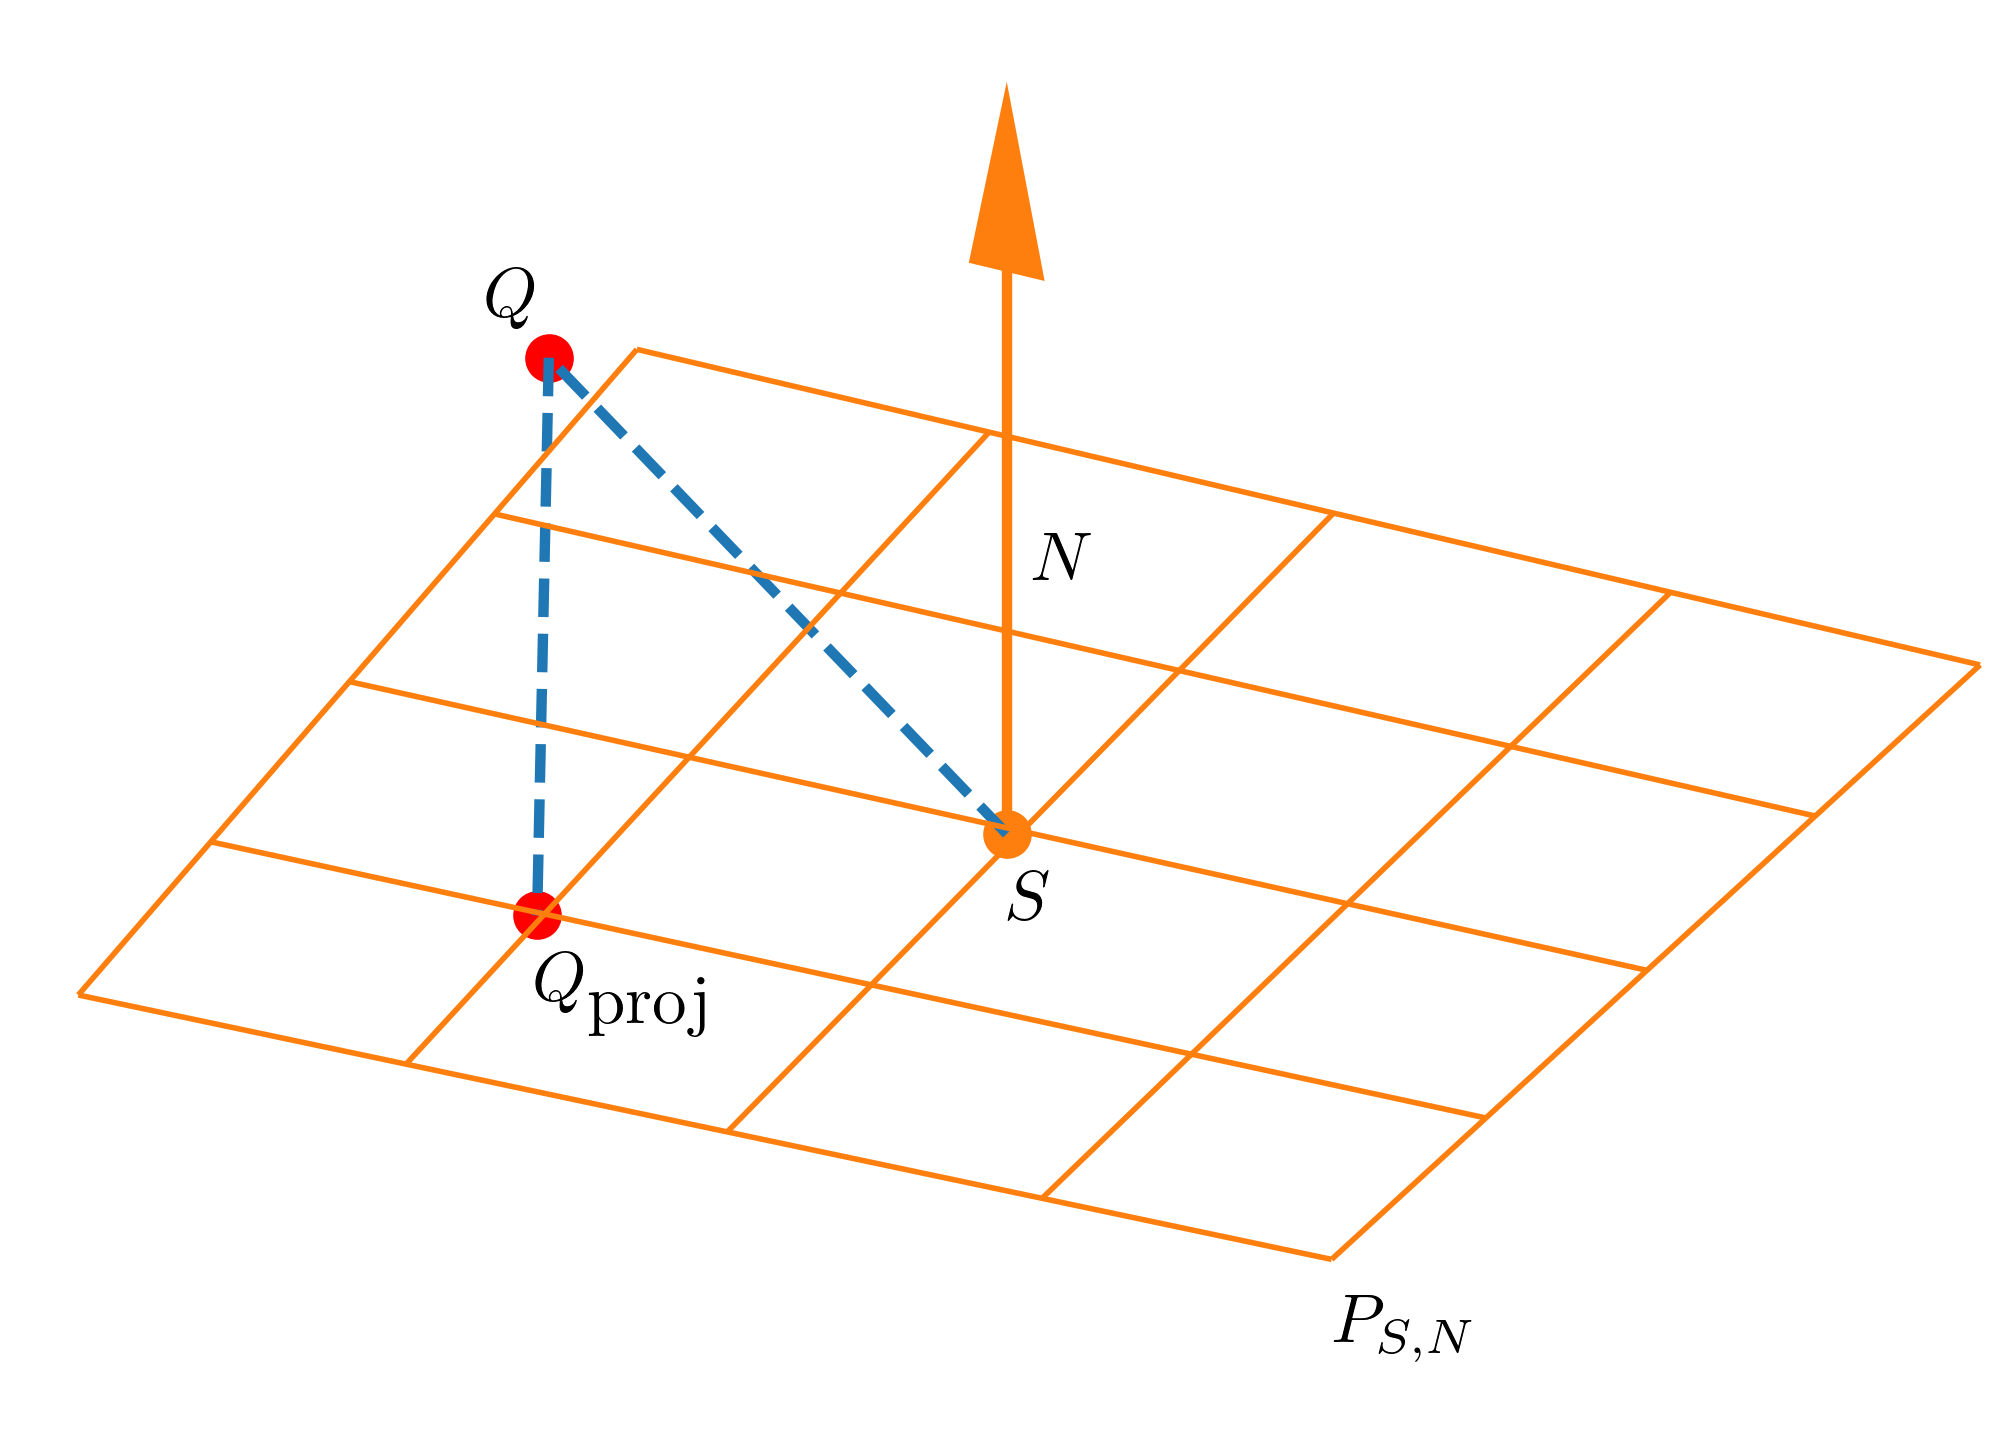
\includegraphics[width=0.4\textwidth]{../python/argh4.png}
		\caption{Projection of a point onto a plane as described by Theorem \ref{thm:planeprojection}.}
	\end{figure}

	In linear algebra, it is often the case that a plane is defined by a support vector and two direction vectors. In CAD it is instead commonplace to use the pair $(S,N)$ of support vector and normal vector. The normal vector is perpendicular to the two direction vectors of the plane. It should be noted that planes, which are two-dimensional affine subspace of $\mathbb{R}^d$, can only be described that way in the case $d = 3$. In our algorithm, the normal vector notation will prove helpful.

	\begin{definition}
		The cross product of two vectors $A, B \in \mathbb{R}^3$ is given by
			$$ A \times B := ||A|| \, ||B|| \, \sin(\theta) \, N,$$
		where $\theta$ is the angle between $A$ and $B$ and $A, B \perp N$ with $||N|| = 1$. Here, $||\cdot||$ is the Euclidean norm of a vector. If $A$ and $B$ are parallel, then $A \times B = 0$
	\end{definition}

	The cross product maps two vectors $A, B$ onto another vector $C$. If $A$ and $B$ are not parallel to each other, then the three vectors $A,B,C$ span $\mathbb{R}^3$. In other words, the cross product maps to a vector that is perpendicular to the two input vectors.

	\begin{theorem}\label{thm:planeequivalence}
		Let $S \in \mathbb{R}^3$ a support vector and $A, B \in \mathbb{R}^3$ two non-parallel direction vectors. Then the plane $\tilde P = \{S + tA + sB : t, s \in \mathbb{R}\}$ can be written as $P_{S,N}$ with 
			$$ N := \frac{A \times B}{||A \times B||}. $$
	\end{theorem}
	\begin{proof}
		Let $X \in \tilde P$. Then
			$$X - S \; \in \; \tilde P - S = \{tA+sB : t,s \in \mathbb{R}\}.$$
		But then because $A, B \perp N$ we have $X-S \in P_{0,N}$, where $0$ is the null vector. Now, 
			$$ X-S+S = X \in P_{0,N} + S = P_{S,N}.$$
	\end{proof}

	As Theorem \ref{thm:planeequivalence} shows, the notation using the pair $(S,N)$ is valid. Given a parametric surface $\beta(u,v)$ with $(u,v) \in [0,1]^2$, we can construct a plane that is tangent to $\beta(u, v)$ for all $(u,v) \in [0,1]^2$ by using the $u$ and $v$ gradients of $\beta$ and taking their cross product. This yields the normal vector of the tangent plane. The support vector of the plane is just equal to the point $\beta(u,v)$. We make the following definition.

	\begin{definition}
		Let $\beta(u,v)$ with $(u,v) \in [0,1]^2$ be a parametric surface that is differentiable in $u$ and $v$. Then the tangent plane of $\beta$ at $(u, v \in [0,1]^2$ is given by the plane
			$$T_{\beta}(u, v) := P_{\beta(u,v), N_{\beta}(u,v)},$$
		where 
			$$N_{\beta}(u,v) := \frac{\nabla_u \beta(u,v) \times \nabla_v \beta(u,v)}{||\nabla_u \beta(u,v) \times \nabla_v \beta(u,v)||}$$
		is the normal vector of the surface $\beta$ at $(u, v)$.
	\end{definition}

	In this section (and in CoolingGen), the surface $\beta(u,v)$ is always differentiable in $u$ and $v$. Suppose we want to intersect the plane $P_{S,N}$ with the parametric surface $\beta(u,v)$ for $(u,v) \in [0,1]^2$. If the surface and the plane do intersect in some point, there exists $(u^{(0)}, v^{(0)}) \in [0,1]^2$ such that $S = \beta(u^{(0)}, v^{(0)})$ is a valid representation for the support vector. If we know such a $(u^{(0)}, v^{(0)})$ a priori, we can find points in the neighborhood of $(u^{(0)}, v^{(0)})$ that also lie in the plane.

	To find a neighboring point, we find the line of intersection $L^{(0)}$ of the tangent plane $T_{\beta}(u^{(0)}, v^{(0)})$ and the target plane $P_{S,N} = P_{\beta(u^{(0)}, v^{(0)}), N}$. Using the normal notation of the planes and the intersection parameter pair $(u^{(0)}, v^{(0)})$, we can easily do this using the following theorem.

	\begin{theorem}
		Let $P_{S, N_1}$ and $P_{S, N_2}$ be two planes with $N_1$ and $N_2$ not parallel. Then
			$$ P_{S, N_1} \cap P_{S, N_2} = L_{S, S+N}(-\infty, \infty), $$
		where $N = \frac{N_1 \times N_2}{|| N_1 \times N_2 ||}$ and $L_{S,S+N}(-\infty, \infty)$ is the line through $S$ and $S+N$. 
	\end{theorem}
	\begin{proof}
		Let $t \in \mathbb{R}$. Notice that $tN \perp N_1$ and $tN \perp N_2$. Therefore, $tN \in P_{0, N_1} \cap P_{0, N_2}$, which is equivalent to $S+tN \in P_{S, N_1} \cap P_{S, N_2}$. But $S+tN = (1-t)S + t(S+N) = L_{S,S+N}(t)$ according to Definition \ref{def:linesegdef}.
	\end{proof}

	The tangent intersection line for the intersection parameters $(u^{(0)}, v^{(0)})$ is equal to
		$$ L^{(0)}(t) = \beta(u^{(0)}, v^{(0)}) + t \cdot \left(\frac{N_{\beta}(u^{(0)}, v^{(0)}) \times N}{||N_{\beta}(u^{(0)}, v^{(0)}) \times N||}\right)$$
	for $t \in \mathbb{R}$. Using an appropriate step size $\alpha \in \mathbb{R}$, we can project the point $L^{(0)}(\alpha) \in T_{\beta}(u^{(0)}, v^{(0)}) \cap P_{\beta(u^{(0)}, v^{(0)}), N}$ onto the surface $\beta$ using the methods from Section \ref{subsec:pointproj} to acquire a candidate for the point $\beta(u^{(1)}, v^{(1)})$. If this point lies outside of the plane $P_{S,N}$, we discard the point, choose a step size less than $\alpha$ and repeat the process. Numerically, we accept a candidate if is within $\epsilon$-distance of te plane $P_{\beta(u^{(0)}, v^{(0)}), N}$ for a small value of $\epsilon > 0$. If $\beta(u^{(1)}, v^{(1)})$ has been found, we repeat this process to find $\beta(u^{(2)}, v^{(2)})$. To do this, we construct $L^{(1)}$ by intersecting $P_{S,N}$ and $T_{\beta}(u^{(1)}, v^{(1)})$ and project $L^{(1)}(\alpha)$ onto $\beta$. We can repeat this iteration step until $|\alpha| < \alpha_0$ for some $\alpha_0 > 0$. If this condition is satisfied, we return the list of the $n$ parameters of intersection, which we can write as $L = \{(u^{(i)}, v^{(i)}): i \in \{1,2,...,n\}\}$.

	\begin{algorithm}[H]
	\begin{algorithmic}[1]
		\Input
			\Desc{$\alpha > \alpha_0$}{step size and minimum step size}
			\Desc{$\xi < 1$}{step size scaling factor}
			\Desc{$\epsilon$}{absolute tolerance}
		\EndInput
		\Output
			\Desc{$\{u^{(i)}, v^{(i)}) : i \in \{1, 2, ..., n\}\}$ }{set of points on the intersection}
		\EndOutput

		\caption{Surface Plane Intersection}\label{alg:surfplaneintersection}
		\Procedure{intersectSurfacePlane}{$\beta, S, N, (u^{(0)}, v^{(0)})$}
			\State $L \gets$ list containing only $(u^{(0)}, v^{(0)})$
			\While {$|\alpha| > |\alpha_0|$}
				\State $(u,v) \gets$ last entry in $L$
				\State $M \gets \left(\frac{N_{\beta}(u, v) \times N}{||N_{\beta}(u, v) \times N||}\right)$
				\State $P \gets \beta(u,v) + \alpha M$
				\State $u_\textrm{proj}, v_\textrm{proj} = \textrm{pointProjection}(\beta, P)$
				\If {$D(\beta(u_\textrm{proj}, v_\textrm{proj}), P_{S,N}) > \epsilon$}
					$\alpha \gets \xi\alpha$
				\Else {} append $(u_\textrm{proj}, v_\textrm{proj})$ to $L$
				\EndIf
			\EndWhile
			\State \Return $L$
		\EndProcedure
	\end{algorithmic}
	\end{algorithm}

	\begin{figure}[H]
		\centering
		\includesvg[width=.8\textwidth]{../python/argh2}
		\caption{Intersection of surface $\beta$ (blue) with the plane $P_{S,N}$ (green). The intersection point $\beta(u^{(0)}, v^{(0)})$ is represented by the red dot. We intersect the tangent plane (orange) of $\beta$ at $(u^{(0)}, v^{(0)})$ with $P_{S,N}$, yielding the line $L^{(0)}$ (black). Near the intersection point, $L^{(0)}$ and the true solution (black dashed curve) are close. The arrows represent the normal vectors.}
		\label{fig:planeintersectionline}
	\end{figure}

	After successfully running Algorithm \ref{alg:surfplaneintersection}, we are left with $n$ points which lie on the intersection curve. We interpolate between these points using NURBS. If necessary, the control points of the NURBS curve can then be projected onto the plane $P_{S,N}$ to ensure that the curve is planar. This scheme proves useful for CoolingGen, because a start parameter pair $(u^{(0)}, v^{(0)})$ is practically always known in this context. Otherwise, a start point can be found using the ray marching technique, which was briefly discussed in Section \ref{subsec:raymarching}.

\chapter{Jet Engine Specific Methods}
	

\section{Fundamental Terms}
	(sauce: books on cooling)
	The creation of cooling geometries inside of turbine blades is not only vital for the enhancement of the thermodynamic efficiency and power output of turbine engines. The materials melting temperature is often exceeded by that of the turbine inlet. To withstand this extreme condition, cooling is required. The blade geometries that we are concerned with in the development of CoolingGen are the ones that succeed the inlet in axial direction.

	CoolingGen creates geometries which lie inside of such a blade surface $B(u,v)$, which is an output of BladeGen, a tool developed by the DLR specifically for the design of blade surfaces. $B(u,v)$ is closed in $u$-direction. For a given $u$, increasing $v$ yields a further distance from the turbines hub. Because of rotational symmetry of the turbine, it is sometimes convenient to describe these geometries in cylindrical coordinates. The transformation from Cartesian coordinates to cylindrical coordinates is given by the map
		$$ Z: (x,y,z) \mapsto (x, \sqrt{y^2+z^2}). $$
	Given the associated circumferential angle $\theta = \arctantwo(y, z)$, the transformation to cylindrical coordinates is invertible.

	\begin{figure}[H]
		\centering
		\begin{subfigure}{.49\textwidth}
			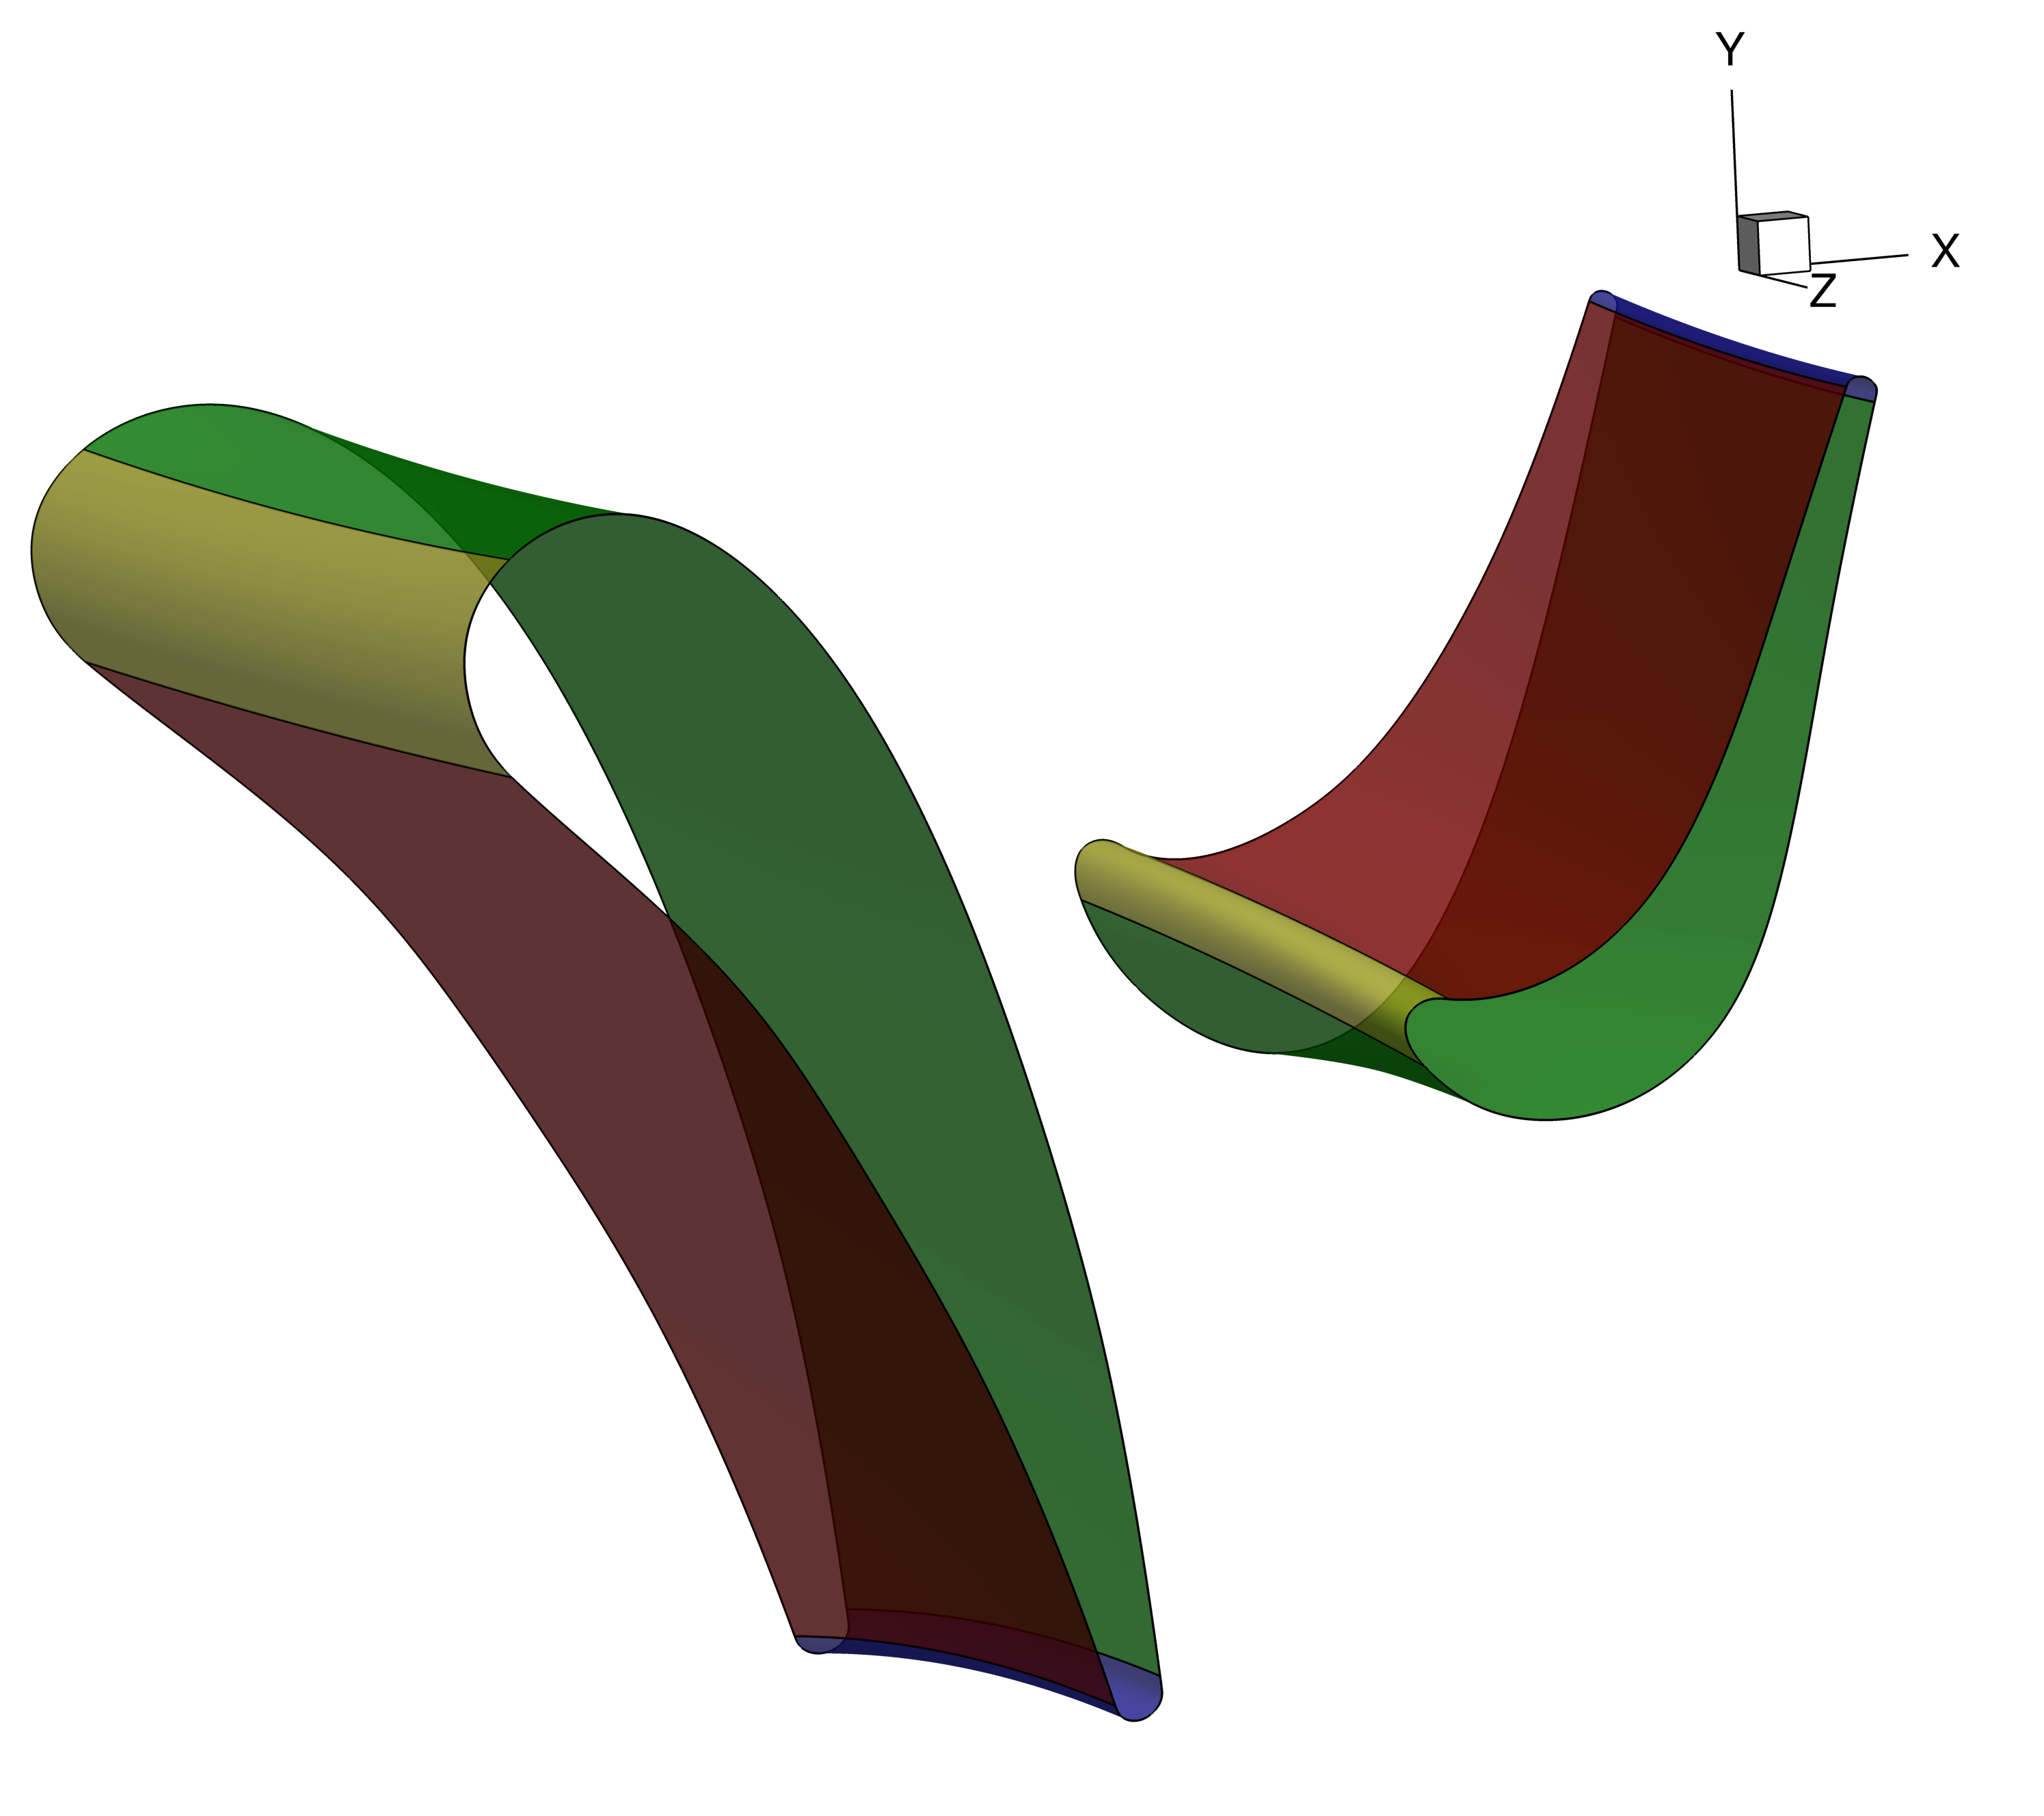
\includegraphics[width=\textwidth]{../tec/rotor_stator/11.png}
			\caption{View on pressure side.}
		\end{subfigure}
		\begin{subfigure}{.49\textwidth}
			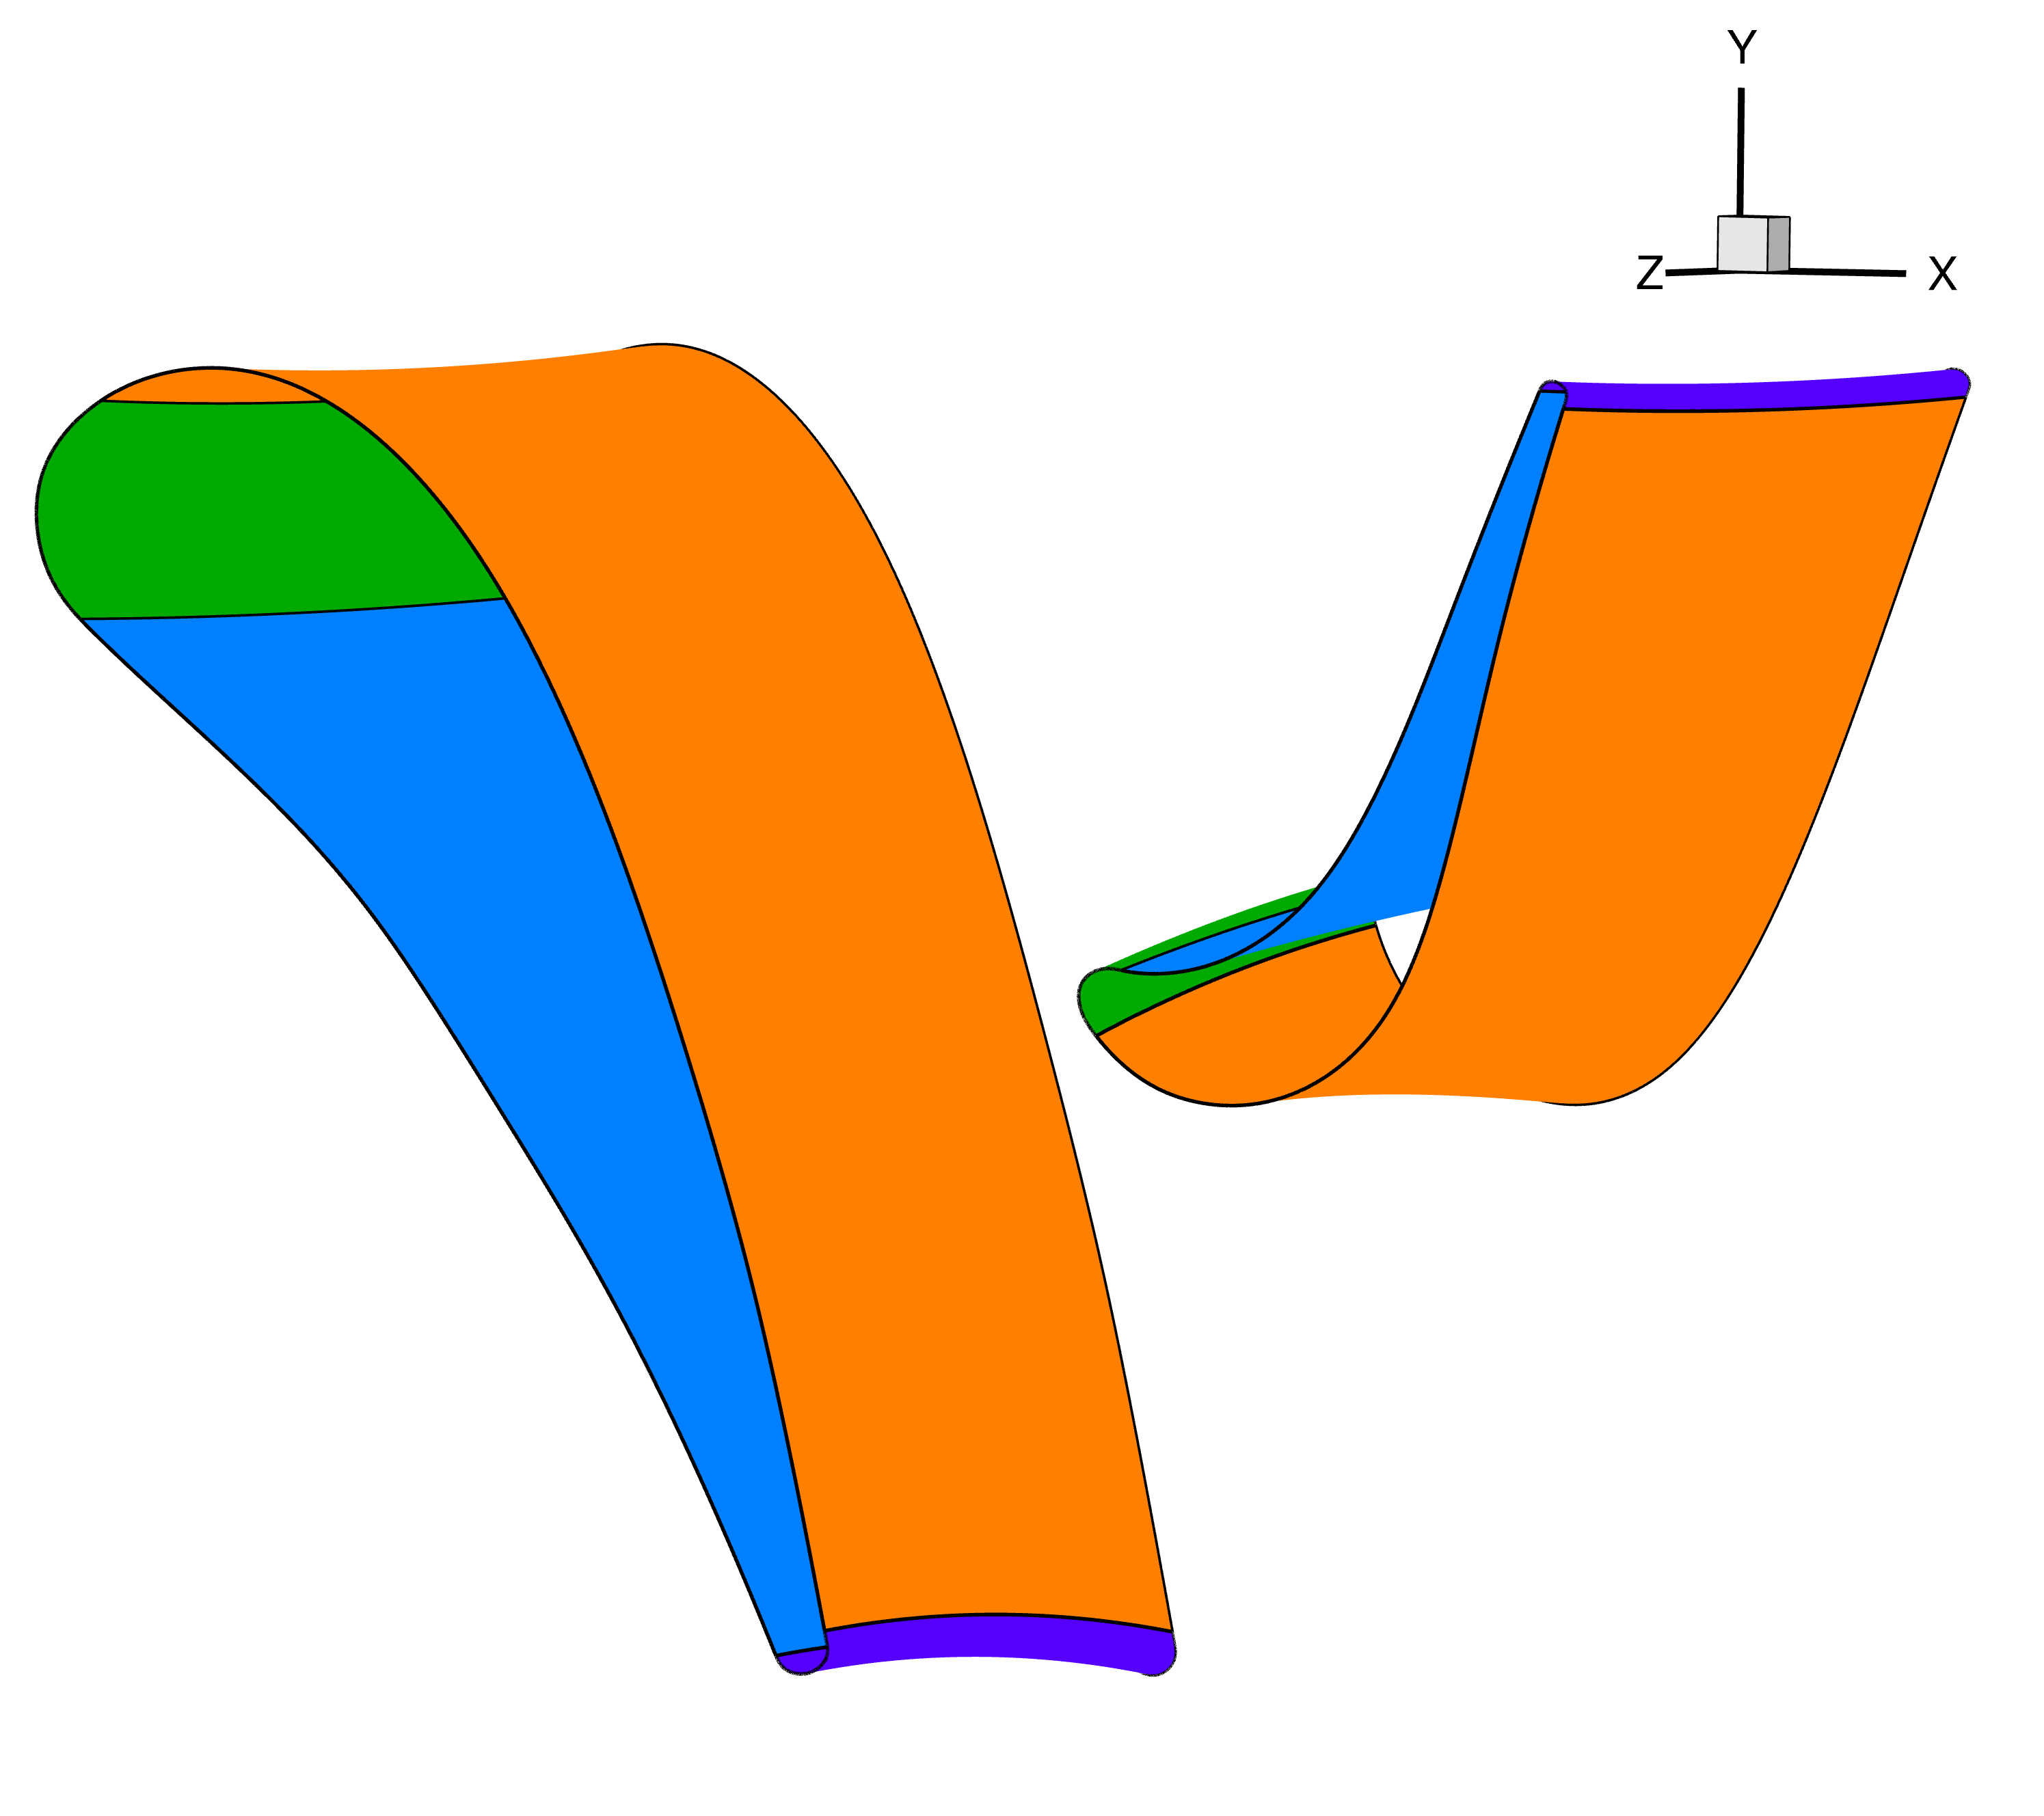
\includegraphics[width=\textwidth]{../tec/rotor_stator/12.png}
			\caption{View on suction side.	}
		\end{subfigure}
		\caption{In (a) and (b), the left is surface represents a stator and the right surface represents a rotor. Yellow marks the leading edge, red the pressure side, green the suction side and blue the trailing edge.}
	\end{figure}

	We make the distinction between two kinds of blades, rotor and stator blades. While the rotor blades rotate around the hub, the stator blades have fixed positions. This was taken into account when designing CoolingGen, so both kinds are currently supported. Furthermor, the blade surface $B(u,v)$ has a named partitioning in $u$-direction into four distinct parts. The leading edge, the suction side, the trailing edge and the pressure side.

\section{The S2 Stream Surface and Stream Surface Coordinates}\label{sec:mrtheta}
	\begin{itemize}
		\item figure of s2m with correct labels
	\end{itemize}

	(source: Wu, 1952 at NACA)
	A stream line is a line that at every point is tangential to the velocity vector field of the flow of the fluid. Its generalization, the stream surface, describes a surface with the same property. The flow in a turbine can be described by a generalization of the stream surface. When designing turbine blades, it is common practice to describe the flow in two families of stream surfaces. These surfaces are called $S_1$ and $S_2$. The $S_1$ surfaces, also known as \emph{blade-to-blade} surfaces, describe the flow behavior between individual blade sections, whereas their counterpart, the $S_2$ surfaces, which are also known as \emph{meridional} surfaces, describe the flow through the turbine.

	\begin{figure}[H]
		\centering
		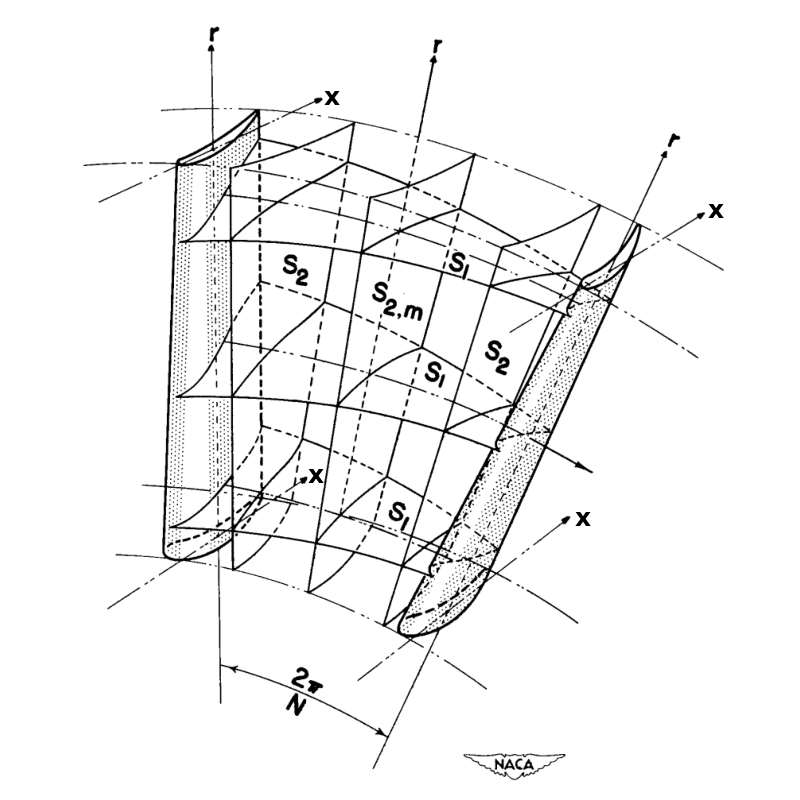
\includegraphics[width=.5\textwidth]{../assets/renamed_wu_naca_s2.png}
		\caption{Example $S_1$ and $S_2$ surfaces of a turbomachine.}
	\end{figure}
	
	Each $S_2$ surface is a parametric surface and therefore a map
		$$s(u,v) : [0,1]^2 \rightarrow \mathbb{R}^3, \quad (u,v) \mapsto (x, r, m),$$
	where $x$ is the axial coordinate, $r = \sqrt{y^2+z^2}$ the distance from the turbine hub and $m$ is the arc length.

	To design the blades for turbomachinery, BladeGen and CoolingGen make use of a certain $S_2$ surface, the so called $S_{2,m}$ surface. This surface lies midway between two blades. Each stream line described by $S_{2,m}$ can then be written as $S_{2,m}(\cdot, v)$. By intersecting the cylindrically transformed $u$-isoparametric curves $Z(B(u,\cdot))$ of the blade with each stream line $S_{2,m}(\cdot, v)$, we can construct a curve $B^{(v)}_\textrm{stream}(u)$ from the intersection points $P_{u,v}$, given by
		$$ B^{(v)}_\textrm{stream}(u) = (m, r\theta, v),$$
	where $m$ is the first argument of $P_{u,v}$, the radius $r$ is equal to the second argument of $P_{u,v}$ and $\theta$ is the circumferential angle and $v$ is constant for each $B^{(v)}_\textrm{stream}$, making the curve planar.
	This coordinate system with respect to arc length $m$ and radius-angle product $r\theta$ is a so called \emph{stream surface coordinate system}. Even though the input blade surface $B(u,v)$ lies in $\mathbb{R}^3$, the most important methods of CoolingGen are operations on objects in this stream surface coordinate system.

\chapter{Results}

\section{Chambers}
	Channels are hollow sections inside a turbine blade which allow for a coolant to pass through. For the construction of channels, we distinguish between straight and curved sections of the channel. The straight sections represent hollow bodies that let the coolant pass in $v$-direction of the turbine blade. These sections are called \emph{chambers}. The curved sections let the coolant pass in $u$-direction of the turbine blade. We call the latter sections \emph{turns}. Inside turns, the coolant flows between chambers. In this section, we present how chambers are constructed, whereas turn construction is thoroughly explained in the next section.

	\begin{figure}[H]
		\centering
		\begin{subfigure}{.32\textwidth}
			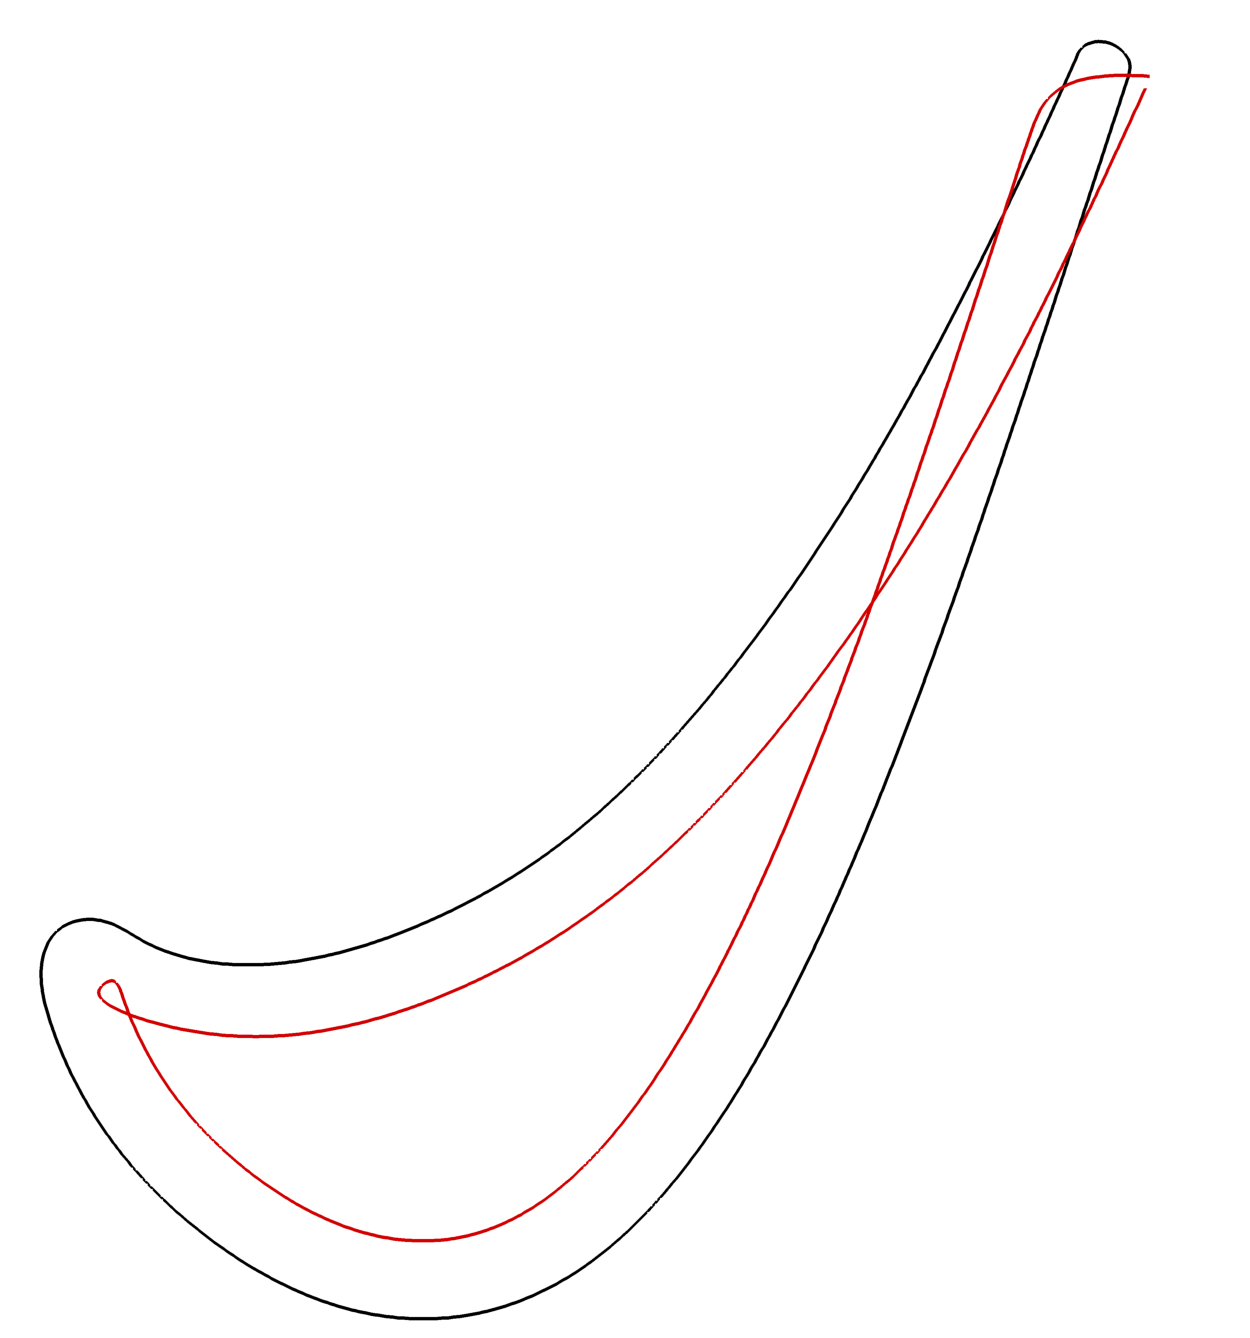
\includegraphics[width=\textwidth]{../tec/shrinking/11.png}
			\caption{Offsetting.}
		\end{subfigure}
		\begin{subfigure}{.32\textwidth}
			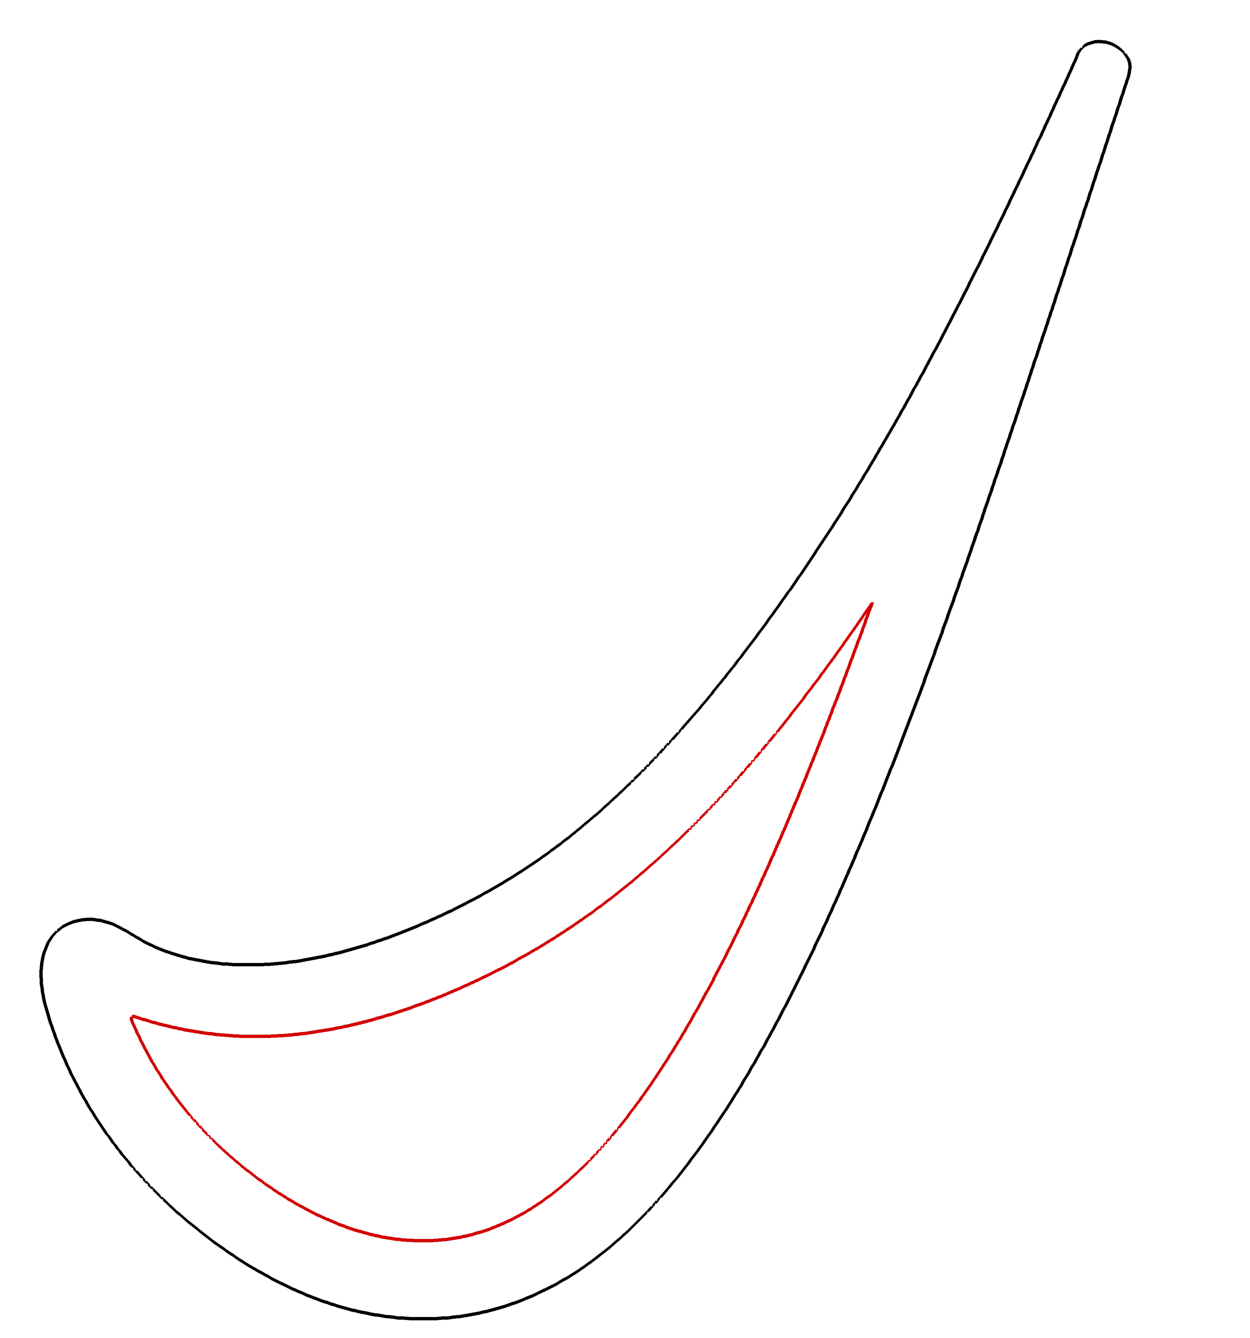
\includegraphics[width=\textwidth]{../tec/shrinking/12.png}
			\caption{Trimming.}
		\end{subfigure}
		\begin{subfigure}{.32\textwidth}
			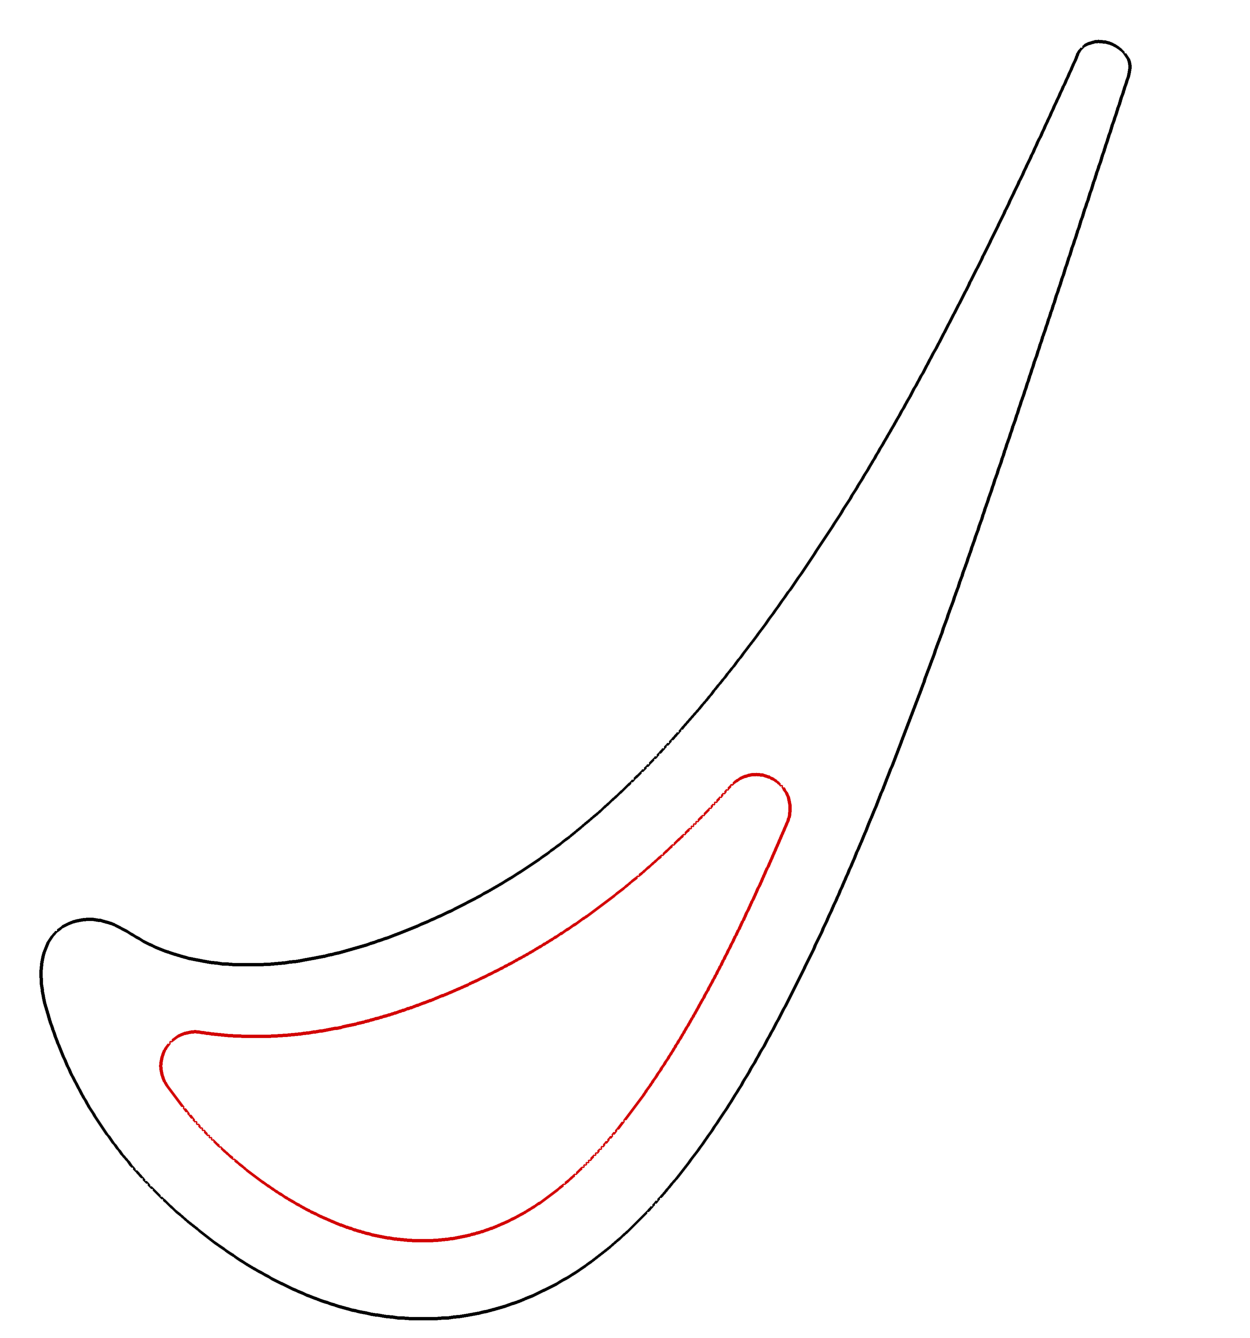
\includegraphics[width=\textwidth]{../tec/shrinking/13.png}
			\caption{Adding fillets.}
		\end{subfigure}
		\caption{Shrinking a profile in $(m, r\theta)$. The black curve represents $B^{(v_i)}_\textrm{stream}(u)$, whereas the red curve in (c) represents $S^{(v_i)}_\textrm{stream}(u)$.}
		\label{fig:profileshrinking}
	\end{figure}

	First, we apply the stream surface coordinate transformation presented in Section \ref{sec:mrtheta} to a fixed number $N$ of $v$-isoparametric curves of the blade to calculate the profiles $B^{(v_i)}_\textrm{stream}(u)$ for $i \in \{1,...,N\}$. These profiles are then offset by an input parameter. The profile is automatically trimmed adequately and fillets are added, the radius of which are also declared as an input. We refer to the resulting profile as \emph{shrunk profile} and declare it $S^{(v_i)}_\textrm{stream}(u)$. This process is depicted in Figure \ref{fig:profileshrinking}.

	\begin{figure}[H]
		\centering
		\includesvg[width=.66\textwidth]{../tec/chambers/walls_labeled.svg}
		\caption{Subdivision of profile along the camber curve. The camber curve is represented by the dashed line.}
		\label{fig:subdivision_chamber}
	\end{figure}

	We calculate the camber curve of each shrunk profile $S^{(v_i)}_\textrm{stream}$. The camber curve $c^{(v_i)}$ is a design aid which is defined by the following property. A point $x$ lies on the camber curve $c^{(v_i)}$ of $S^{(v_i)}_\textrm{stream}$ if and only if for some $d$ its offset curve $O^{S^{(v_i)}_\textrm{stream}}_d$ has a self intersection at $x$. Along the camber curve, we define the wall input, which is given by a sorted set of parameters $w_j$ representing the positions of each wall relative to the camber curve, $j \in \{1,...,N_C-1\}$, where $N_C$ is the number of chambers that shall be created. For each position, we also define an angle $\omega_i$. Each position-angle pair represents two rays
		$$ c(w_j) + sR_{\omega_j} \nabla c(w_j) \quad\text{and}\quad c(w_j) - sR_{\omega_j} \nabla c(w_j) $$
	for $s \in [0, \infty)$, where $R$ is a rotation matrix like the one presented in Equation (\ref{eq:rotationmat}). Using the Algorithm \ref{alg:raymarching}, we can find the intersection $p_j^+$ and $p_j^-$ of the rays and the profiles. The line segment $\overline{p_j^+p_j^-}$ now represents the $j$-th wall. 

	The blade is then partitioned at these intersection points. For each such partitioning, we are left with four curves per chamber profile. Some of these curves are the walls, which are curves that represent straight lines between $p_j^+$ and $p_j^-$. There are four distinct cases. The first case is $N_C = 1$. In this case, the four curves are given by the pressure side, the leading edge, the suction side and the trailing edge partitioning of the input blade surface $B(u,v)$. If however $N_C > 1$, we have three more cases. The chamber profile located at the leading edge, which we refer to as leading chamber profile, consists of the partition of the pressure side between the leading edge and $p_1^+$, the leading edge, the partition of the suction side between the leading edge and $p_1^-$ and lastly the first wall curve. The chamber profile located at the trailing edge, which we refer to as trailing chamber, consists of the partition of the pressure side between trailing edge and $p_{N_C-1}^+$, the $(N_C-1)$-th wall, the partition of the suction side between trailing edge and $p_{N_C-1}^-$ and the trailing edge. For the $j$-th chamber profile, where $j \neq 1$ and $j \neq N_C-1$, these four curves are the partition of the pressure side between $p_j^+$ and $p_{j+1}^+$, the $j$-th wall, the partition of the suction side between $p_{j}^-$ and $p_{j+1}^-$ and the $(j+1)$-th wall. This procedure is exemplified in Figure \ref{fig:subdivision_chamber}.

	\begin{figure}
		\begin{subfigure}{.32\textwidth}
			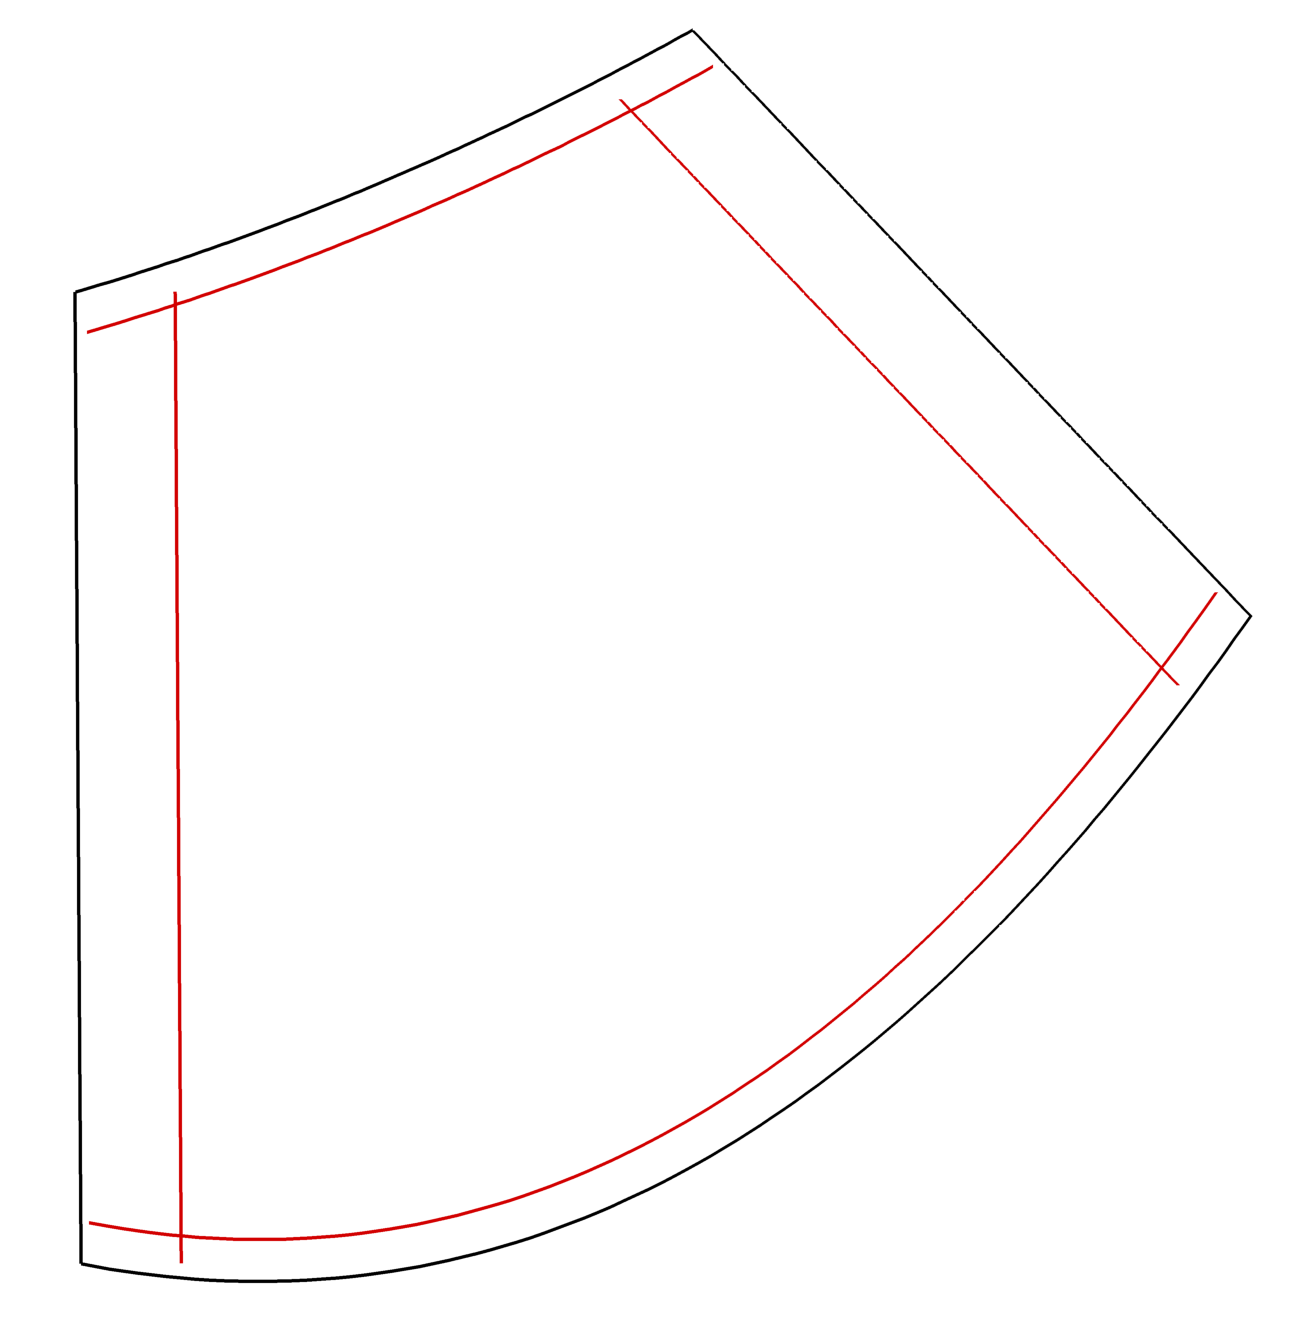
\includegraphics[width=\textwidth]{../tec/chambers/11.png}
			\caption{Offsetting.}
		\end{subfigure}
		\begin{subfigure}{.32\textwidth}
			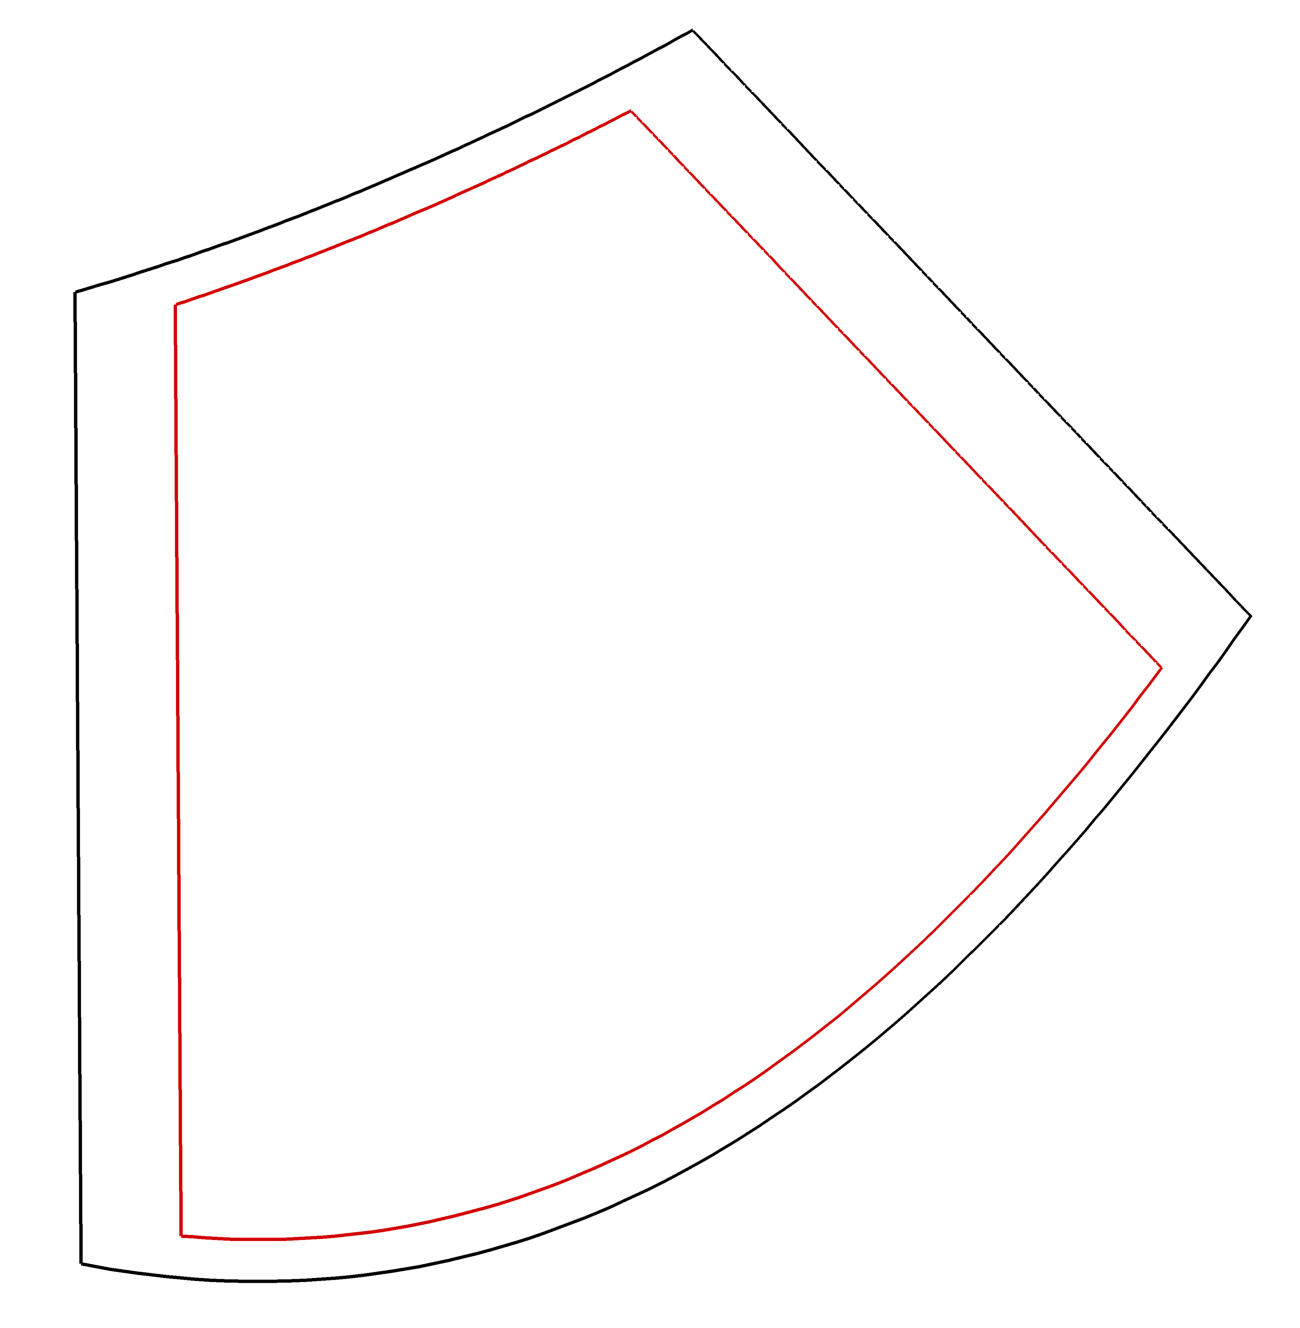
\includegraphics[width=\textwidth]{../tec/chambers/12.png}
			\caption{Trimming.}
		\end{subfigure}
		\begin{subfigure}{.32\textwidth}
			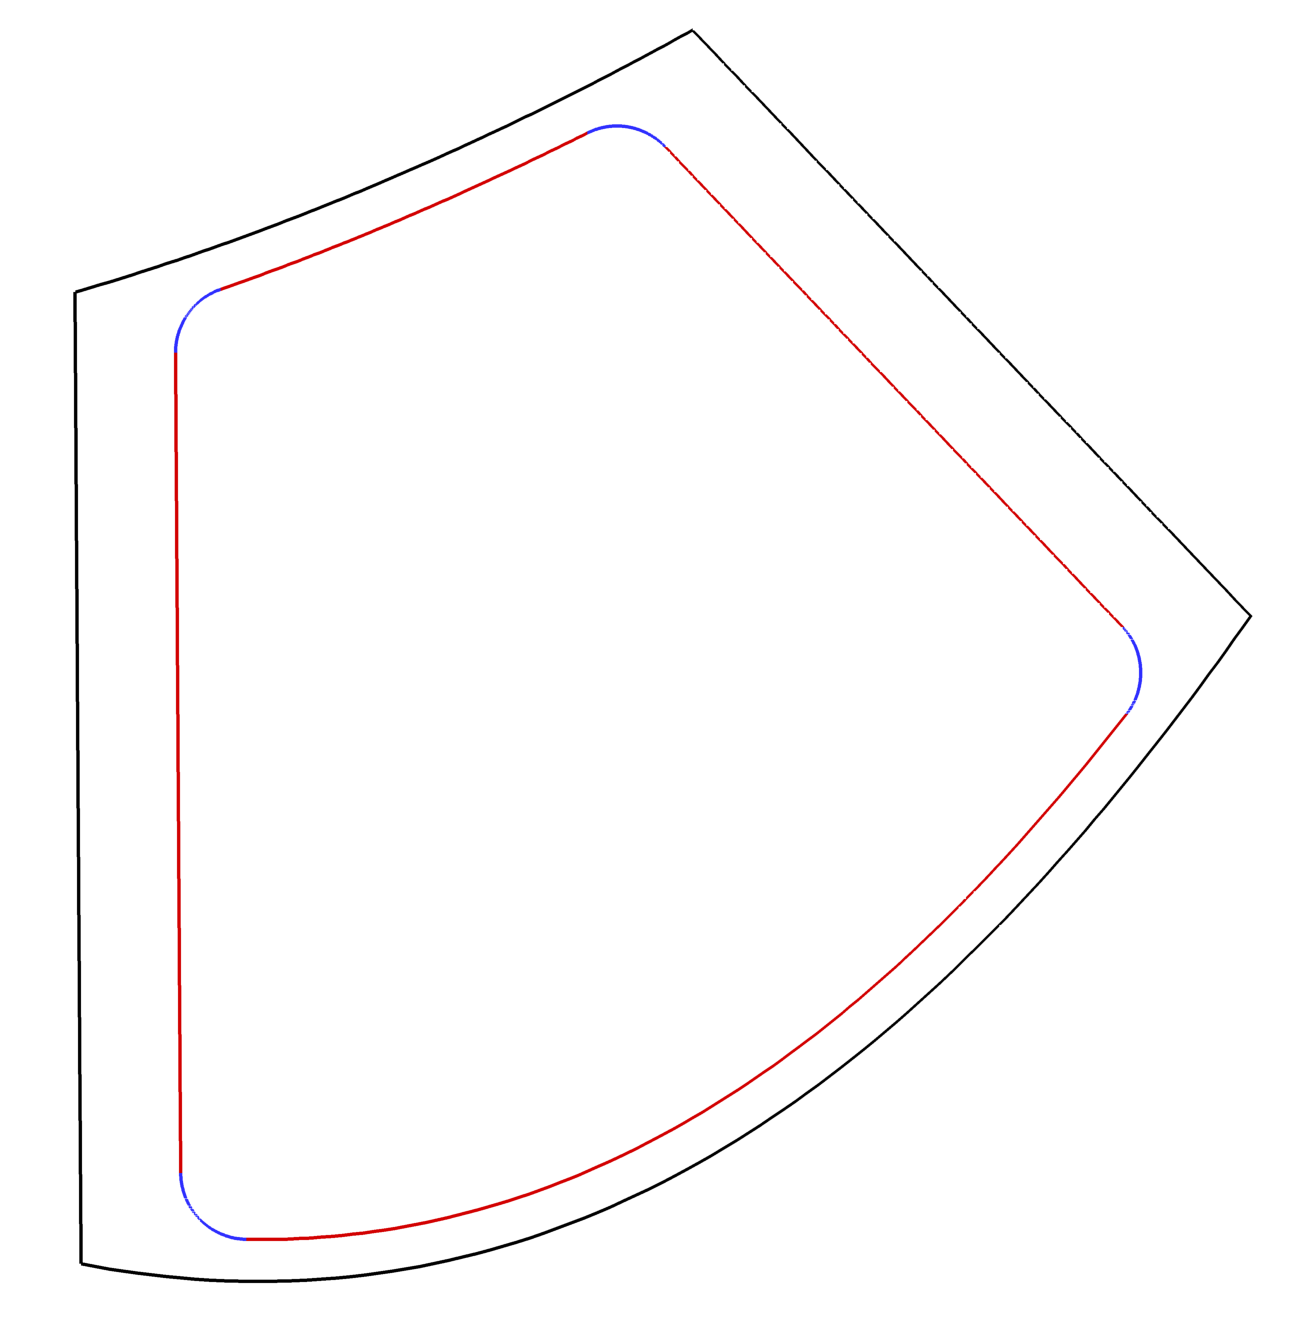
\includegraphics[width=\textwidth]{../tec/chambers/13.png}
			\caption{Adding fillets.}
		\end{subfigure}
		\caption{Construction of a chamber profile.}
		\label{fig:chamber_shrinking}
	\end{figure}

	After performing this partitioning, we can offset the curves. However, each curve is offset differently. In the wall input, the thickness of the wall in each direction is specified as an input. In fact, this input specification is done using NURBS curves. For each partition, the user of CoolingGen specifies control points $(v_k, d_k)$, where $v_k \in [0,1]$ is the surface parameter and $d_k$ is the respective thickness with $k \in [1, ..., K]$. The leading and trailing profile offsets are linearly interpolated between suction and pressure side offsets to guarantee differentiability of the chamber profile at the leading and trailing edge transitions, respectively. Since after offsetting, the four chamber profile parts do not necessarily align, we connect the curve ends either by curve-curve intersection, ray-curve intersection or ray-ray intersection, depending on which one is applicable. The rays are in this case defined by $R_{A,B}$, where $A$ represent the curve boundary points and $B$ represent the gradient at the curve boundary points.

	After connecting and trimming the offset curves using the methods in Section \ref{sec:offsetcurves}, we are left with four trimmed offset curves that intersect non-differentiably at their boundary points. We apply the fillet curve method presented in Section \ref{sec:filletcurves}. These steps can be seen in Figure \ref{fig:chamber_shrinking}.

	\begin{figure}[H]
		\centering
		\begin{subfigure}{.55\textwidth}
			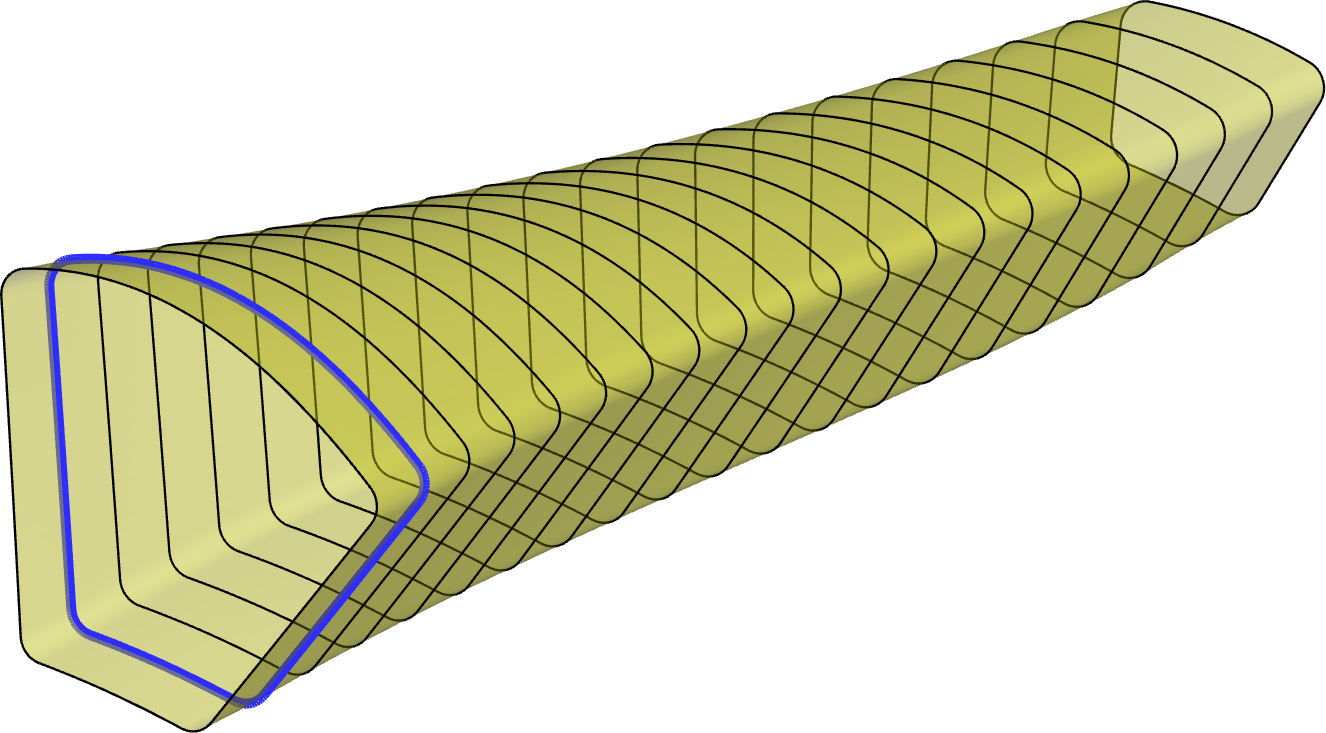
\includegraphics[width=\textwidth]{../tec/lifting/lifted.png}
			\vspace{1cm}
			\caption{A single chamber.}
		\end{subfigure}
		\phantom{aa}
		\begin{subfigure}{.41\textwidth}
			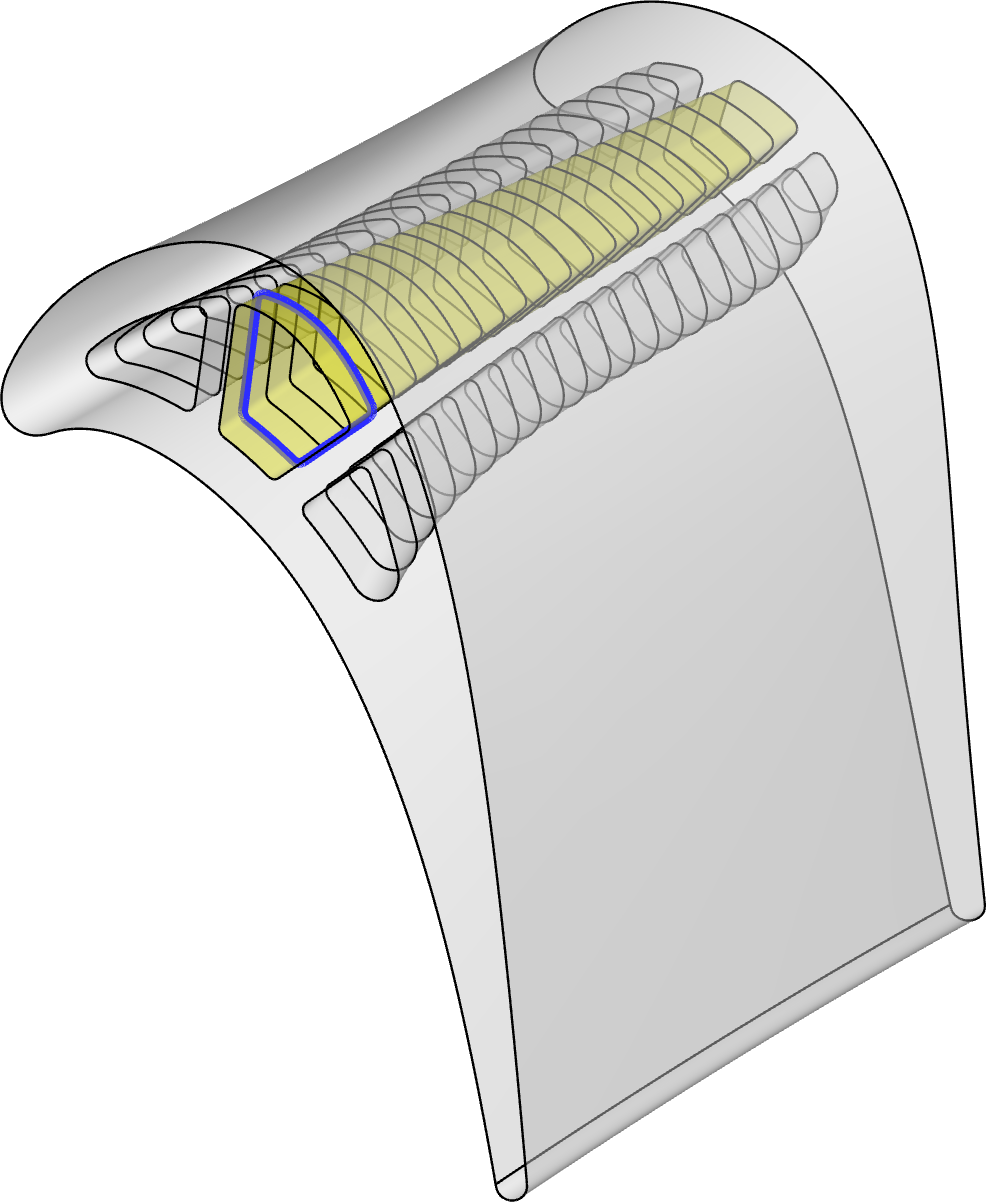
\includegraphics[width=\textwidth]{../tec/lifting/complete.png}
			\caption{Three chambers inside of blade surface.}
		\end{subfigure}
		\caption{Lifted chamber surfaces.}
	\end{figure}
	
	We can use the inverse coordinate transformation from the $(m, r\theta)$ stream surface coordinate system to the Cartesian coordinate system. Interpolation between the transformed chamber profiles yields $N_C$ many three-dimensional chamber surfaces.

\section{Turns}
	\begin{figure}[H]
		\centering
		\begin{subfigure}{.48\textwidth}
			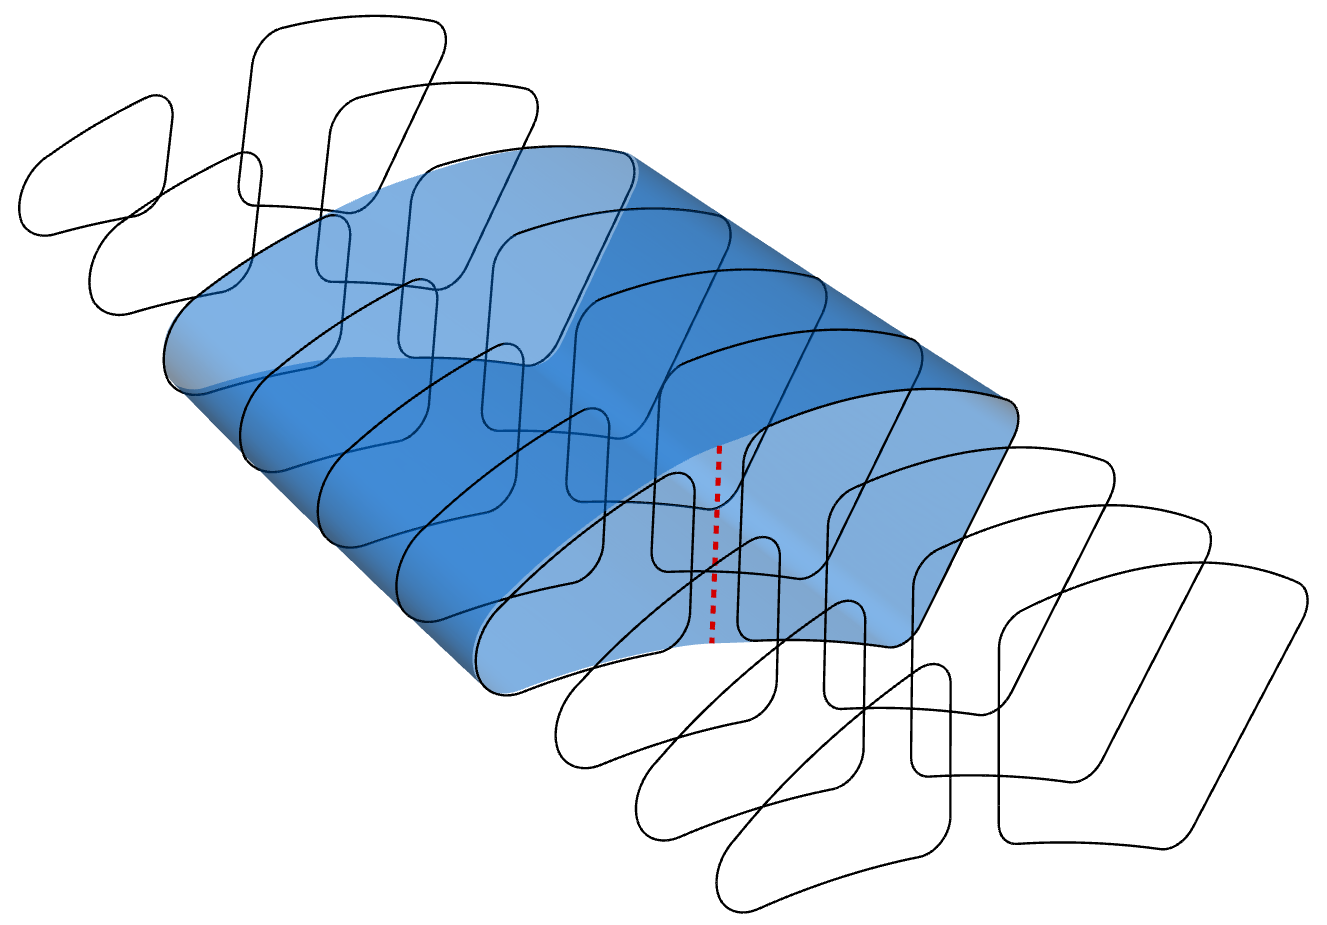
\includegraphics[width=\textwidth]{../tec/turn/12.png}
			\caption{Combining the chambers. The axis of rotation is marked in red.}
		\end{subfigure}
		\phantom{aa}
		\begin{subfigure}{.48\textwidth}
			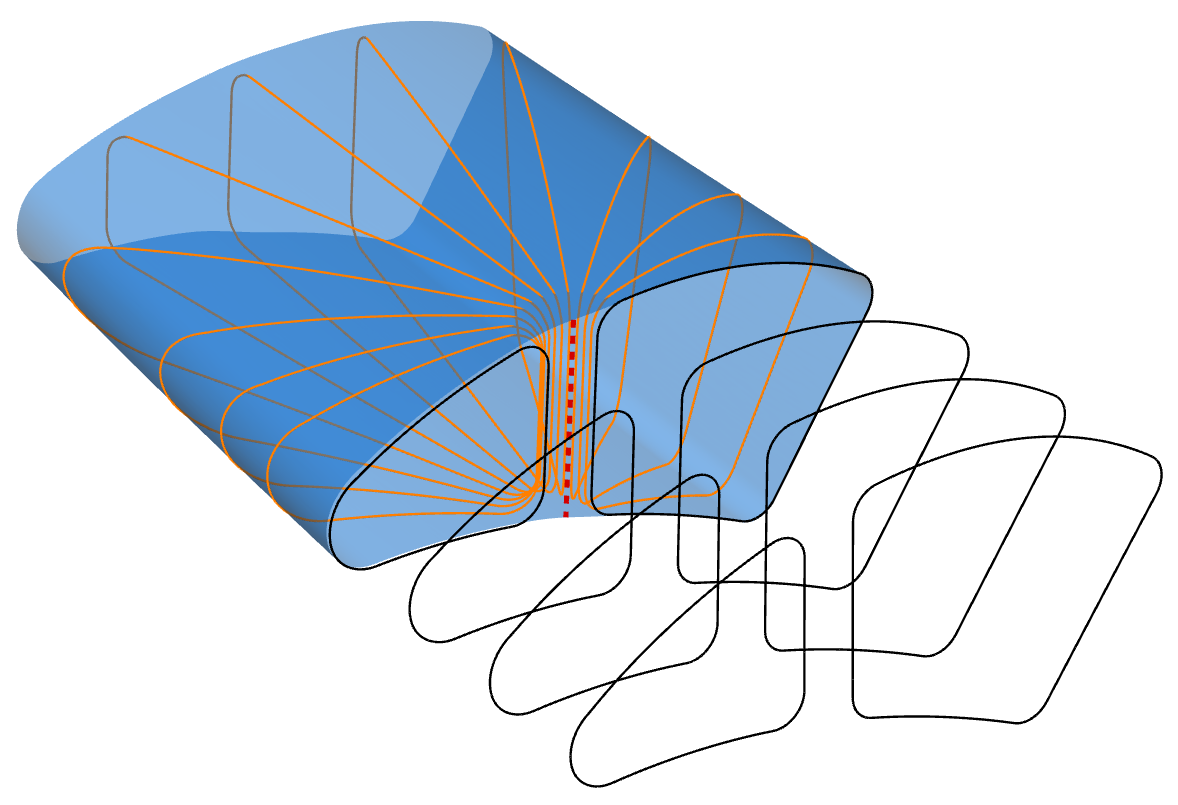
\includegraphics[width=\textwidth]{../tec/turn/11.png}
			\caption{Intersecting the combined surface with affine planes that contain the axis of rotation.}
		\end{subfigure}
		\caption{Construction of a turnaround.}
	\end{figure}

	\begin{figure}[H]
		\centering
		\begin{subfigure}{.4\textwidth}
			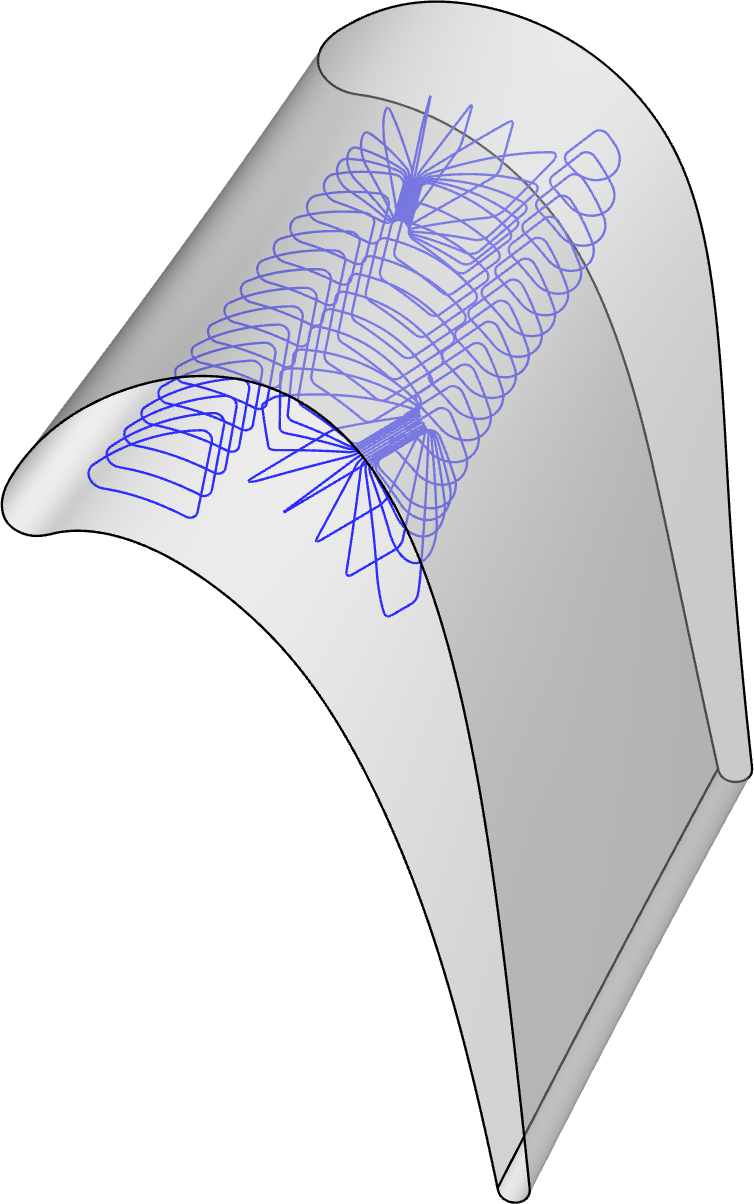
\includegraphics[width=\textwidth]{../tec/channel/13.png}
			\caption{Channel profiles.}
		\end{subfigure}
		\begin{subfigure}{.4\textwidth}
			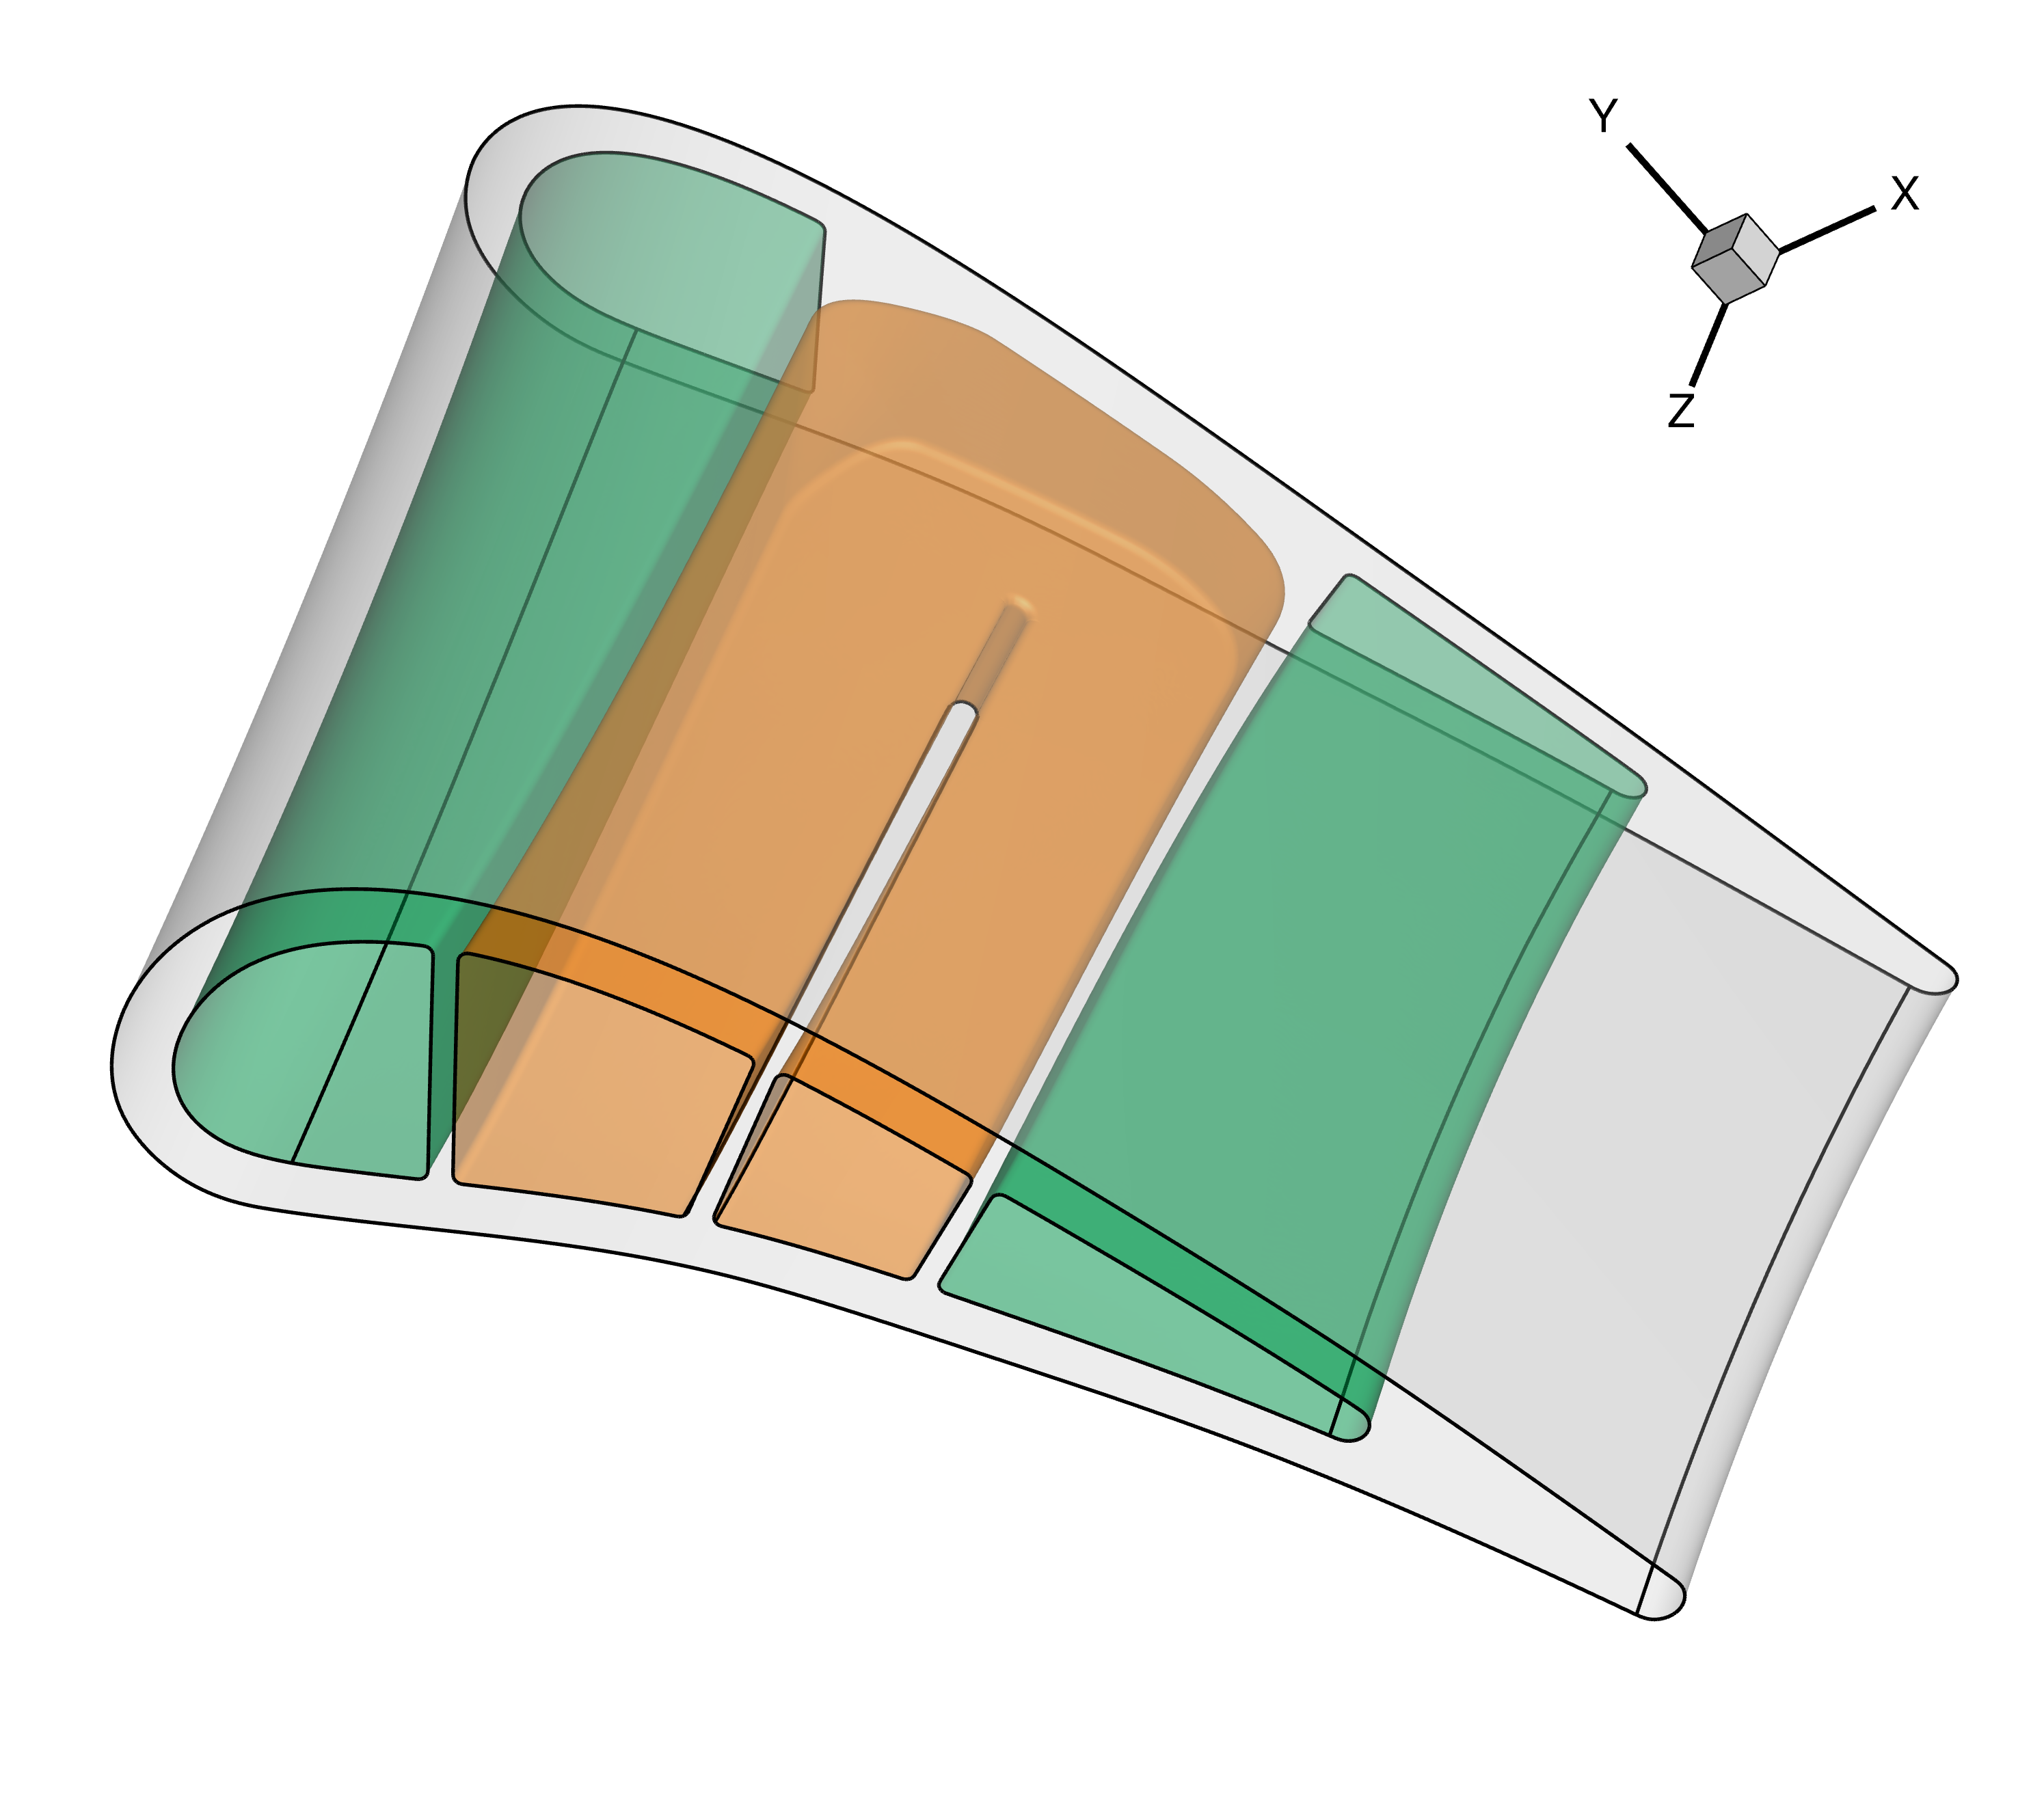
\includegraphics[width=\textwidth]{../tec/channel/14.png}
			\caption{Channel surface.}
		\end{subfigure}
		\caption{Cooling channel with three chambers and two turnarounds.}
	\end{figure}


\section{Film Cooling Holes}
	\begin{itemize}
		\item parametric definitions of delimiting curves
		\item explain how these are made
		\item then explain how they are basically made out of rays and how that is helpful with intersections
	\end{itemize}

	\begin{figure}[H]
		\centering
		\begin{subfigure}{.15\textwidth}
			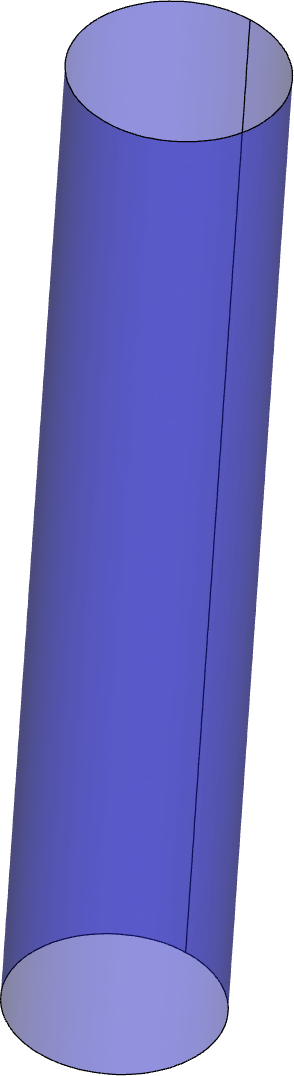
\includegraphics[height=6cm]{../tec/holes/16.png}
			\vspace{1.5cm}
			\caption{Cylindrical.}
		\end{subfigure}
		\phantom{aa}
		\begin{subfigure}{.19\textwidth}
			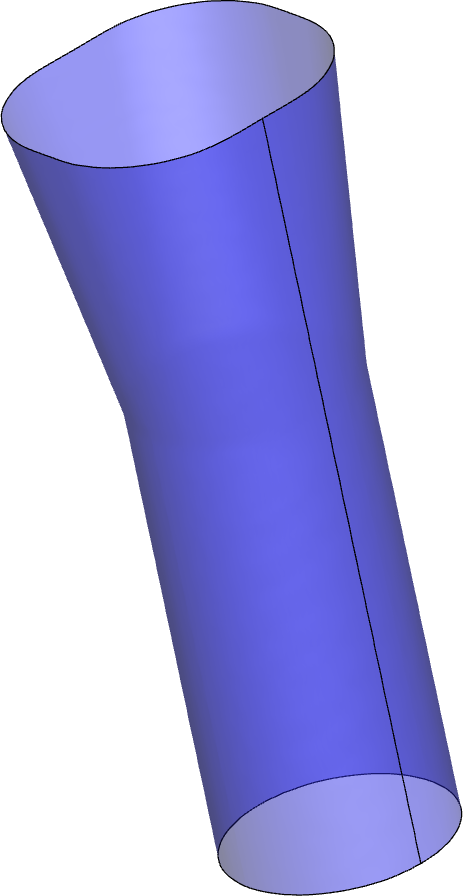
\includegraphics[height=6cm]{../tec/holes/15.png}
			\vspace{1.1cm}
			\caption{Fan shaped.}
		\end{subfigure}
		\begin{subfigure}{.55\textwidth}
			\includesvg[width=\textwidth]{../python/fanshapedCurveDefinition}
			\caption{Delimiting curves.}
		\end{subfigure}
		\caption{Film cooling holes and their delimiting curves}
	\end{figure}


\section{Impingement Inserts}
\section{Slots}
\section{Export for CENTAUR}
\section{Export for Open CASCADE}

\chapter{Discussion}
\section{Future Work}
\section{Conclusion}
\cite{Piegl1997}

% Bibliography, numbered and formatted like a chapter (for the TOC as well)
\printbibliography[heading=bibnumbered, title=References]

\end{document}